\chapter{Ripple Phase}
When the temperature is reduced from the fluid phase, 
the ripple phase is observed in bilayers consisting of DMPC and DPPC lipids.
This chapter discusses X-ray scattering experiments on the ripple phase 
formed by dimyristolphosphatydylcholine (DMPC) bilayers. 

%%%%%%%%%%%%%%%%%%%%%%%%%%%%%%%%%%%%%%%%%%%%%%%%%%%%%%%%%%%%%%%%%%%%%%%%%%%%%%%
\section{Introduction}
(At some point, do some literature search and write up this section)
The ripple phase has been a fascinating thermodynamic phase to many physicists 
and physical chemists since its discovery. It was originally observed in 
calorimetry study for alcanes by sturevant. Although this phase has never been reported to 
occur in a biologically relevant situation, it provides an interesting opportunity
to study fundamental lipid interactions and their influence on the bilayer 
shape. (Let's find some recent papers and see if anyone says anything about
biological relevance)

In the first structural study of this phase by Tardieu \textit{et al.},
the X-ray diffraction pattern from DLPC was phased by a pattern recognition
technique and the electron density map was calculated. It was shown that the structure
corresponds to a 2D oblique unit cell shown in Fig.~\ref{fig:unit_cell}.
The calculated 
electron density map showed that DLPC bilayers are height modulated
and have a smooth, asymmetric shape. 
The ripple wavelength $\lambda_r$ was reported to be 85.3 \AA, 
the lamellar periodicity $D$ 55.3 \AA, and the oblique angle
$\gamma$ 110\textdegree. 
The electron density map reported the ripple amplitude $A$ = 15 \AA\ in DLPC.

Various experiments have indicated the existence of two types of ripple phases:
the stable asymmetric and the metastable symmetric phase. In the asymmetric
phase, a plane of reflection perpendicular to the ripple wave vector is 
absent. The metastable symmetric phase has been seen in DPPC bilayers, but not
in DMPC.

\begin{figure}[htbp]
  \centering
  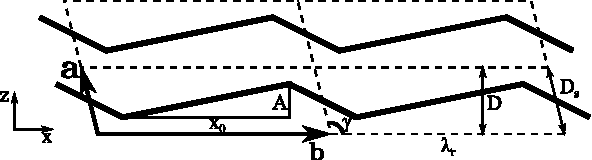
\includegraphics[width=0.8\textwidth]{figures/ripple/unit_cell}
  \caption{Lattice structure of the asymmetric ripple phase. Unit cells are shown in
  dash lines. Center of bilayers are shown by thick, solid lines. Notations 
  in the figure are ($\mathbf{a}$ and $\mathbf{b}$: lattice unit vectors),
  ($D$: $D$-spacing along $z$), ($\lambda_r=|\mathbf{b}|$: ripple wavelength), 
  ($\gamma$: oblique tilt angle), ($A$: ripple amplitude),
  ($\psi$: chain tilt angle with respect to the $z$ direction),
  and ($x_\textrm{M}$: projected length of the major arm).}
  \label{fig:unit_cell}
\end{figure}

The equilibrium structure of the ripple phase has been extensively studied by
X-ray diffraction \cite{ref:Janiak76,ref:Janiak79,ref:Tardieu73,ref:Wack89,ref:Yao91,ref:Sun96,ref:Cunningham98},
neutron diffraction \cite{ref:Mortensen88,ref:Bradshaw89}, 
AFM \cite{}, freeze fracture electron microscopy \cite{ref:Woodward96},
and freeze fracture scanning tunneling microscopy \cite{} techniques.
In the scanning tunneling microscopy experiment \cite{ref:Zasadzinski88}, 
the three-dimensional contours of the ripple phase $P_{\beta'}$ of
dimyristoylphophatidylcholine (DMPC) were imaged, and
a ripple wavelength of 130 \AA\ and an amplitude of 45 \AA\ were reported.

\textcolor{red}{multilayer vs LUV. Any LUV paper report on ripple?}

From X-ray data of the DMPC ripple of unoriented samples, 
Wack and Webb \cite{ref:Wack89} argued that the ripples have a sawtooth shape,
but were unable to phase the observed pattern.
Their X-ray form factor data were later
phased by employing a modeling and fitting technique by Sun \textit{et al.}
\cite{ref:Sun96}, and the electron density map was calculated, which indicated that  
the ripples indeed have a sawtooth shape. The map also showed that
the major arm is about twice as long as the minor arm. The bilayer
thickness was found to be larger than that of the minor arm. The
value of the bilayer thickness in the major arm was comparable to the
thickness of DMPC bilayers in the gel phase whereas the thickness
of the minor arm was comparable to that in the fluid phase.

A structural investigation by X-ray diffraction of the ripple phase of
oriented dipalmitoylphosphatidylcholine (DPPC) samplesindicated that
hydrocarbon chains are packed in a hexagonal lattice with chains
tilted in the plane perpendicular to the ripple wave vector \cite{ref:Hentschel91}.
In that study, the oblique angle $\gamma$ was found to be 90\textdegree.

\textcolor{red}{Katsaras and Raghnathan papers}

Several MD (molecular dynamics) simulations have been carried out, indicating
various lipid packing. de Vrie \textit{et al.} has suggested interdigitated chain in the
minor side \cite{ref:deVries05}.

\textcolor{red}{Some theory papers}

\begin{table}[htbp]
\centering
  \begin{tabular}{ccc}
    \hline
    $D$ & $\lambda_r$ & $\gamma$ \\
    (\AA) & (\AA) & (deg) \\
    \hline
    55.0 & 159.4 & 99.0 \\
    57.0 & 140.8 & 97.6 \\
    57.3 & 151.6 & 97.8 \\
    57.4 & 148.4 & 97.6 \\
    57.5	 & 144.1 & 97.8 \\
    57.5 & 141.9 & 98.0 \\
    58.0 & 140.1 & 98.2 \\
    \textcolor{blue}{57.8} & \textcolor{blue}{145.0} & \textcolor{blue}{98.2} \\
    58.0 & 141.7 & 98.4 \\
    59.8 & 129.6 & 97.3 \\
    60.6 & 130.1 & 97.0 \\
    61.5 & 130.8 & 96.5 \\
    62.4 & 122.0 & 95.9 \\
    63.9 & 123.1 & 94.9 \\
    64.9 & 120.3 & 92.3 \\    
    \hline 
  \end{tabular}
  \caption{Lattice constants for DMPC at $T$ = 18.0 \textcelsius\
  reported by Wack and Webb \cite{ref:Wack89}. The data collected and analyzed in this thesis
  are colored blue.} 
\end{table}

%%%%%%%%%%%%%%%%%%%%%%%%%%%%%%%%%%%%%%%%%%%%%%%%%%%%%%%%%%%%%%%%%%%%%%%%%%%%%%%
\section{Materials and Methods}
\subsection{Sample Preparation}
DMPC was purchased from Avanti Polar Lipids and used without further purification.
Oriented thin films were deposited on clean silicon wafers with
a chloroform:methanol 2:1 (volume ratio) mixture following the rock and roll procedure
\cite{Tristram-Nagle07_MMB}.
In previous synchrotron experiments, the samples were created and annealed 
more than a week in advance and stored in a refrigerator. The quality of 
these samples measured by their mosaic spread was found to worsen over time
after the samples were annealed. Therefore, to ensure the best sample quality, the 
samples were annealed for approximately 12 hours just before the X-ray experiment.
Figure~\ref{fig:annealing_chamber} shows a picture of the annealing chamber. 
To achieve gentle but efficient hydration of a sample, filter papers were installed. 
For successful annealing, it must be emphasized that the annealing 
chamber should equilibrate in an annealing oven prior to putting a sample in the chamber.
When a sample was put in the chamber sitting at a room temperature and
then the system was placed inside the oven, warmer water vapor inside the chamber 
condensed on the cooler sample, causing so called flooding of oriented sample. 
A small drop of water on an oriented film is detrimental for the orientation quality because the
entropy-driven formation of unilamellar vesicles causes oriented bilayers to peel off
one by one. 

\begin{figure}[htbp]
  \centering
  %\includegraphics[scale=\textwidth]{figures/ripple/}
  \caption{A picture of an annealing chamber. Need to take a picture}
  \label{fig:annealing_chamber}
\end{figure}

The sample for the grazing incident wide angle study was prepared in the same way 
as for low angle study. In order to minimize the geometric broadening, the 
sample was trimmed to 1 mm in width along the beam direction.

The sample for transmission study was deposited on a thin, 35 micron, silicon
wafer, and oriented following the rock and roll procedure \cite{Tristram-Nagle07_MMB}. 
See also Sec.~\ref{sec:volume_method}. 
Because the wafer was very fragile, attaching the sample to a sticky 
thing was impossible. Instead, the sample was attached to a plastic cap on 
a small vial with a small amount of heat sink compound at a corner of the 
wafer. The wafer was stable enough for rocking. 

%%%%%%%%%%%%%%%%%%%%%%%%%%%%%%%%%%%%%%%%%%%%%%%%%%%%%%%%%%%%%%%%%%%%%%%%%%%%%%%
\subsection{Instrumental Resolution}
Talk about divergence, dispersion, and geometric broadening.
\subsubsection{Divergence}

\subsubsection{Energy dispersion}
multilayer vs Si crystal

\subsubsection{Geometric Broadening}
WAXS vs LAXS
Make a table (in pixel and q)

\begin{table}[htbp]
  \centering
  \begin{tabular}{ccc}
    \hline
    
  \end{tabular}
\end{table}

\subsection{Low Angle X-ray Scattering Experiment}\label{sec:LAXS_method}
(Transmission was in 2011)
The low resolution X-ray scattering experiment was carried out at the Cornell 
High Energy Synchrotron Source (CHESS) G1 station in three different runs
(2011, 2012, and 2013). The low angle X-ray scattering (LAXS) data analyzed 
in this thesis were collected in 2013.
The X-ray beam was set up by the station scientist, Dr. Arthor Woll.
A W/B$_4$C multilayer monochromater with energy bandwidth $\Delta E$/$E$ of 1.5\% was used,
providing a very intense X-ray beam. 
The energy of the X-ray beam was 10.55 keV, corresponding to a wavelength 
of 1.175 \AA. 
The horizontal and vertical divergence of the beam were
$4.2 \times 10^{-5}$ rad and $1.6 \times 10^{-4}$ rad, respectively.
The beam shape, measured through a semi-transparent 200 $\mu$m thick
molybdenum (Mo) beam stop, is shown in Fig.~\ref{fig:ripple_lr_beamx}
and \ref{fig:ripple_lr_beamz}.
The horizontal beam width was 2.3 pixels (0.16 mm). The vertical beam
width was approximately 1 mm, tall enough to cover the entire sample
when the sample was tilted by 7\textdegree. The sample was rocked
during X-ray exposure between -1.6\textdegree\ and 7\textdegree\ 
in order to observe many diffraction peaks in one data collection. 
The sample to detector distance was 359.7 mm, measured by indexing
silver behenate Bragg peaks. The D-spacing of silver behenate is known to be
58.367 \AA.

\begin{figure}[htbp]
  \centering
  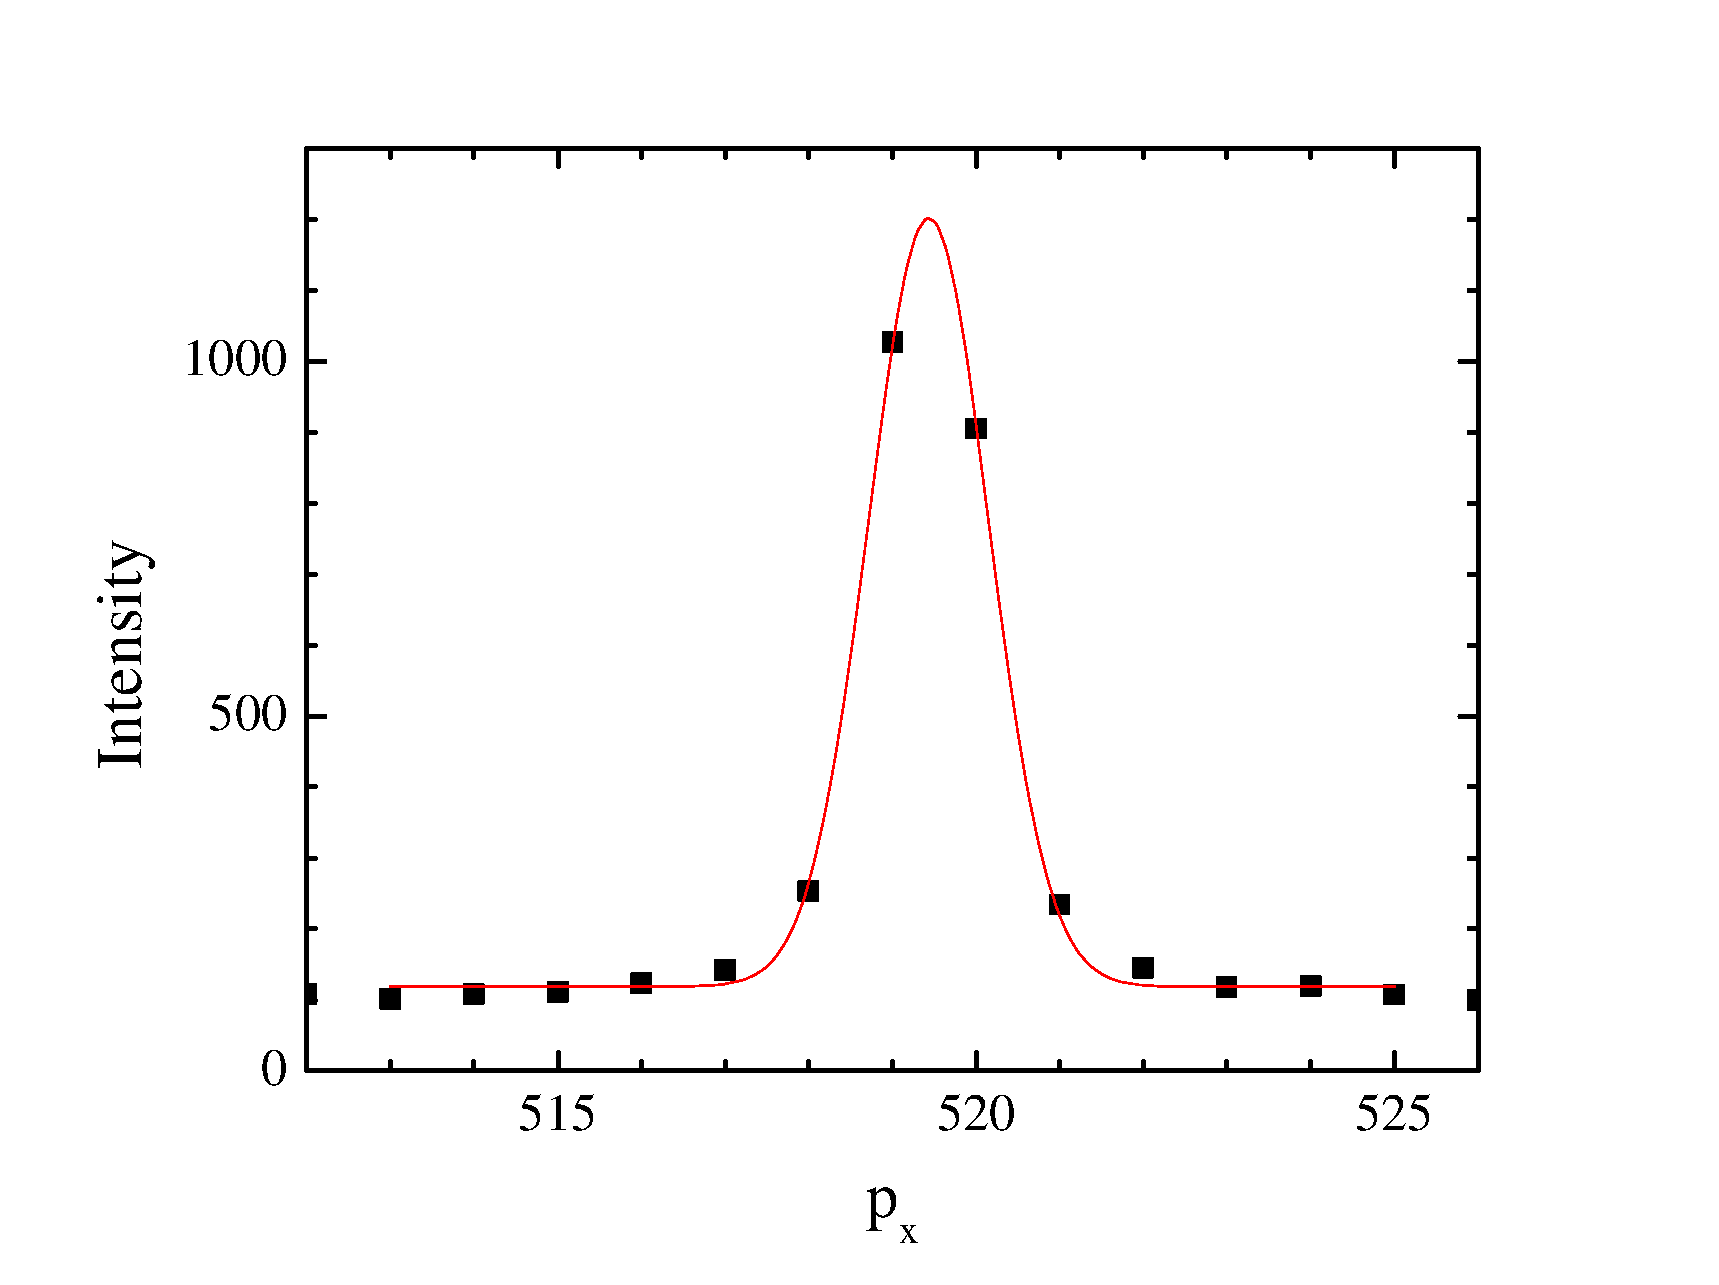
\includegraphics[width=0.7\textwidth]{figures/ripple/MMs/laxs/beamx_lr}
  \caption{The horizontal profile of the beam used in the low resolution study.
  Each pixel was 0.07113 mm, which gave a CCD angular resolution $\Delta\theta$ of 
  0.0057\textdegree, corresponding to $\Delta q=0.0011$ \AA$^{-1}$ at the 
  sample to detector distance of 359.7 mm. 
  The beam FWHM = 1.7 pixels, giving $\Delta\theta = 0.010$\textdegree\ or
  $\Delta q= 0.0019$ \AA$^{-1}$.}
  \label{fig:ripple_lr_beamx}
\end{figure}

\begin{figure}[htbp]
  \centering
  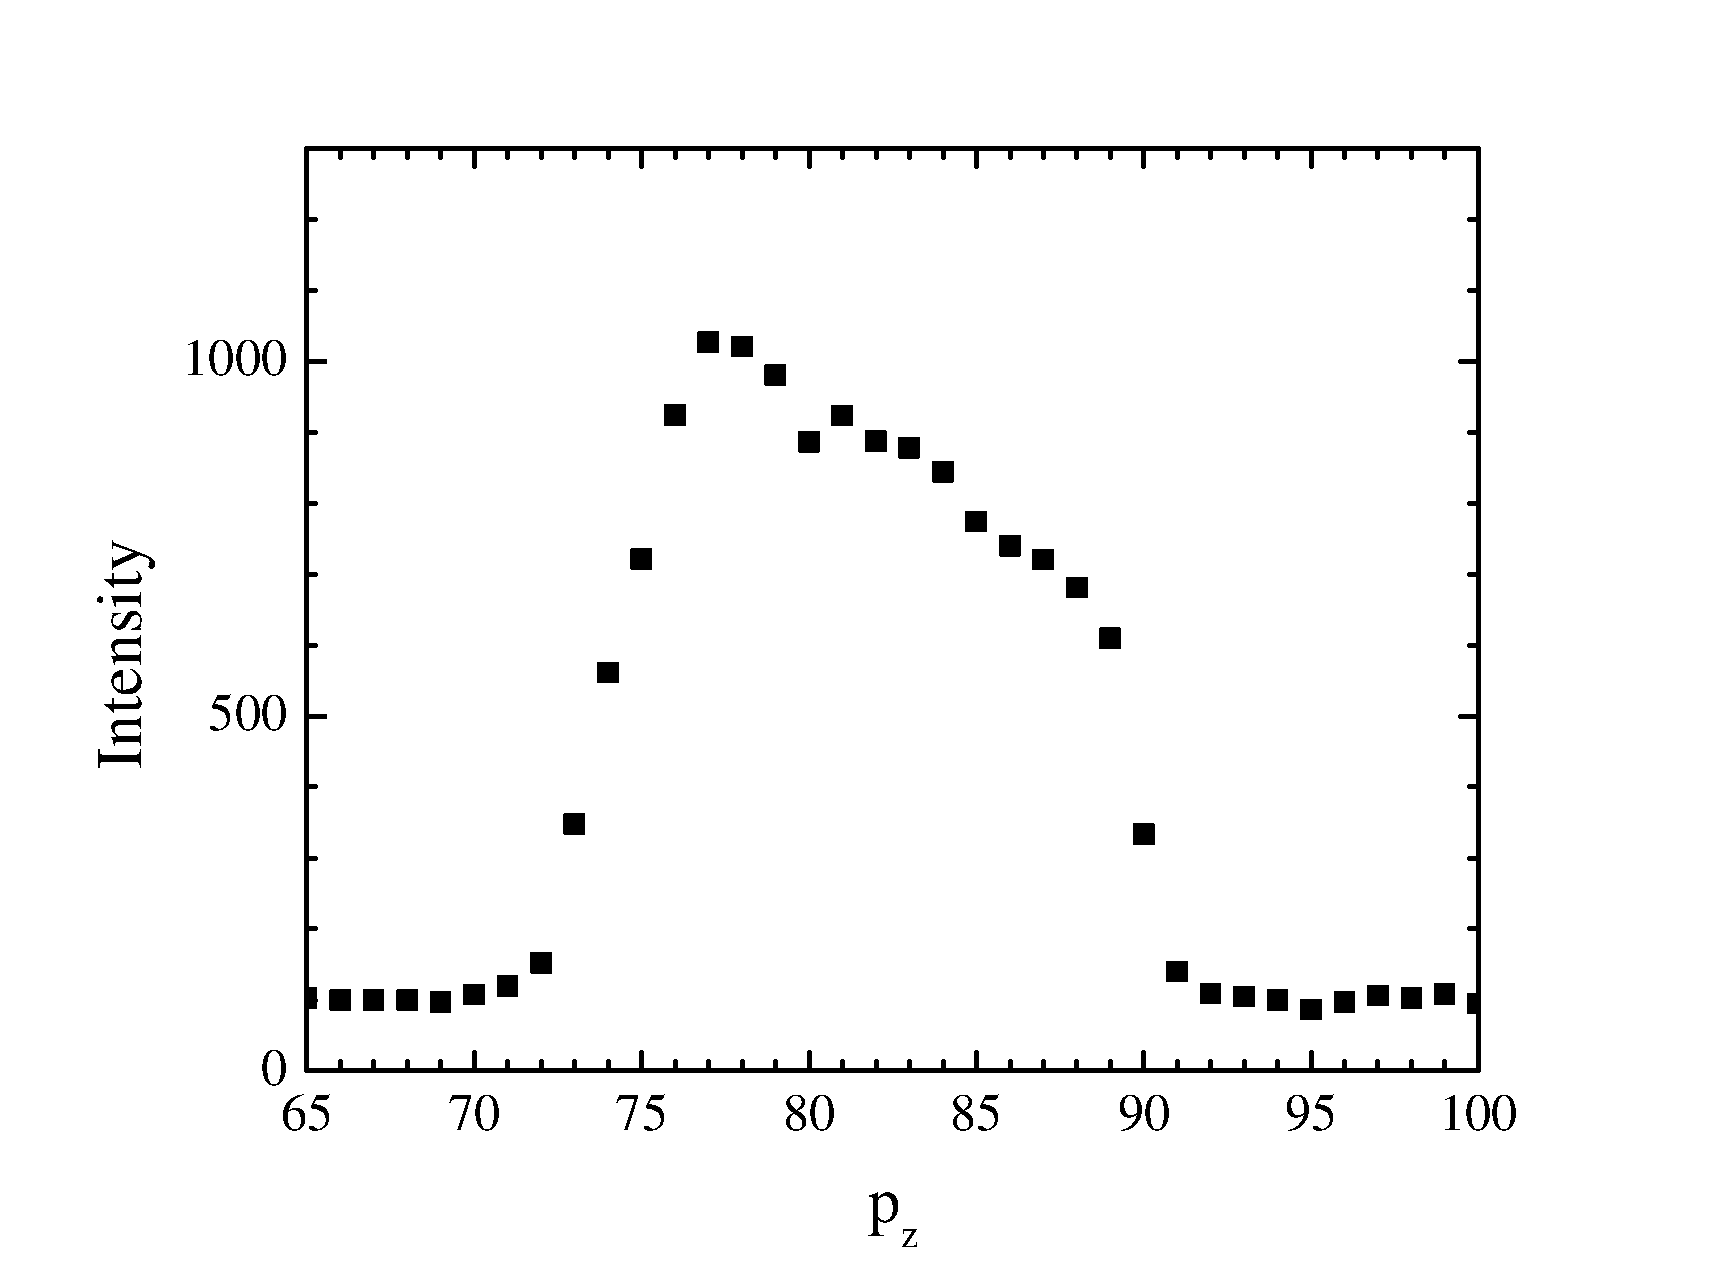
\includegraphics[width=0.7\textwidth]{figures/ripple/MMs/laxs/beamz_lr}
  \caption{The vertical profile of the beam used in the low resolution study.
  The beam height = 15 pixels = 1.1 mm.}
  \label{fig:ripple_lr_beamz}
\end{figure}

Occasionally, sheets of molybdenum (Mo), each nominally 25 $\mu$m were 
used to attenuate the incoming beam. 
These sheets were installed by Dr. Arthur Woll in the upstream of the sample chamber.
The attenuation length $\mu$ of 10.55 keV X-ray in Mo is 13.74 $\mu$m \cite{ref:cxro}.
%8 keV X-ray in Mo is 6.433 $\mu$m
For a 25 $\mu$m thick Mo attenuator, the attenuation factor is calculated to be
$[\exp(-25/13.74)]^{-1} = 6.2$. The exact attenuation factor was determined
by comparing X-ray images collected with and without the attenuator, 
shown in Fig.~\ref{fig:olddopc} and \ref{fig:attenuator}.
The attenuation factor of the nominally 25 $\mu$m thick Mo was found to 
be 6.9 for the wavelength used (1.175 \AA). 

Sheets of Mo were also used as a beam stop downstream of the sample, just 
outside the hydration chamber, to attenuate the beam and strong orders.
100 and 200 $\mu$m were used to attenuate strong orders and 
and 225 $\mu$m to attenuate the beam. To avoid saturation of CCD pixels by
the very intense beam, the beam stop was always set to block the beam.

A few Bragg peaks in the low angle X-ray scattering of the ripple phase
were very strong, leading to saturation of CCD pixels for data collection
with a long exposure time. 
In order to probe a wide range of $q$-space, three images were taken:
1) a short, one second exposure with a nominally 25 micron 
molybdinum attenuator installed in the upstream of the sample to reduce the intensity
of the incoming X-ray beam, 2) one second exposure without the beam attenuator,
and 3) 60 second exposure with a beam stop blocking the very intense 
(1,0) and (2,0) peaks. See Fig.~\ref{fig:ripple_laxs_images}. 
Then, the integrated intensity of (1,0) peak was measured
from the first image. This value was multiplied by 6.9 to account for the beam
attenuation and by 60 to scale with the exposure time. 
The intensity of (2,0) and (2,-1) were measured from the second image, also
multiplied by 60 to account for the shorter exposure time. The intensity of
the rest of the observed peaks were measured from the third image.

The integrated intensity of each peak was obtained using the Nagle lab tview
software developed by Dr. Yufeng Liu \cite{Liu03} by putting a box around a
peak and summing up the intensity in those pixels that fall inside the box.
The background scattering was estimated by measuring the intensity in pixels
near the peak but not containing any peak tail. The choice of box size was 
made according to the width of each peak. Because of mosaic spread in the sample,
the peaks were wider for higher orders. 
Consequently, the box was made wider for higher
orders. The box size was chosen so that approximately 80\% of the peak intensity
was counted toward the integrated intensity.



\begin{figure}[htbp]
  \centering
  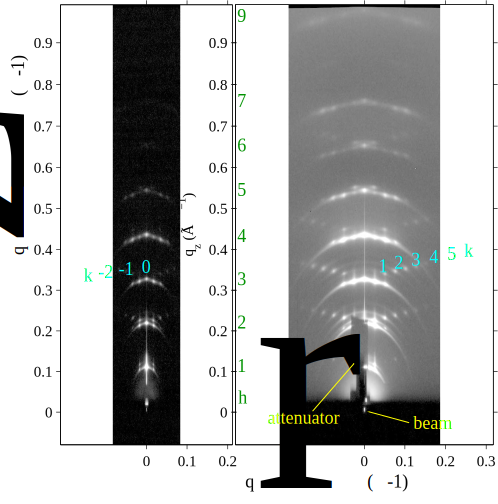
\includegraphics[width=0.95\textwidth]{figures/ripple/ripple083and085}
  %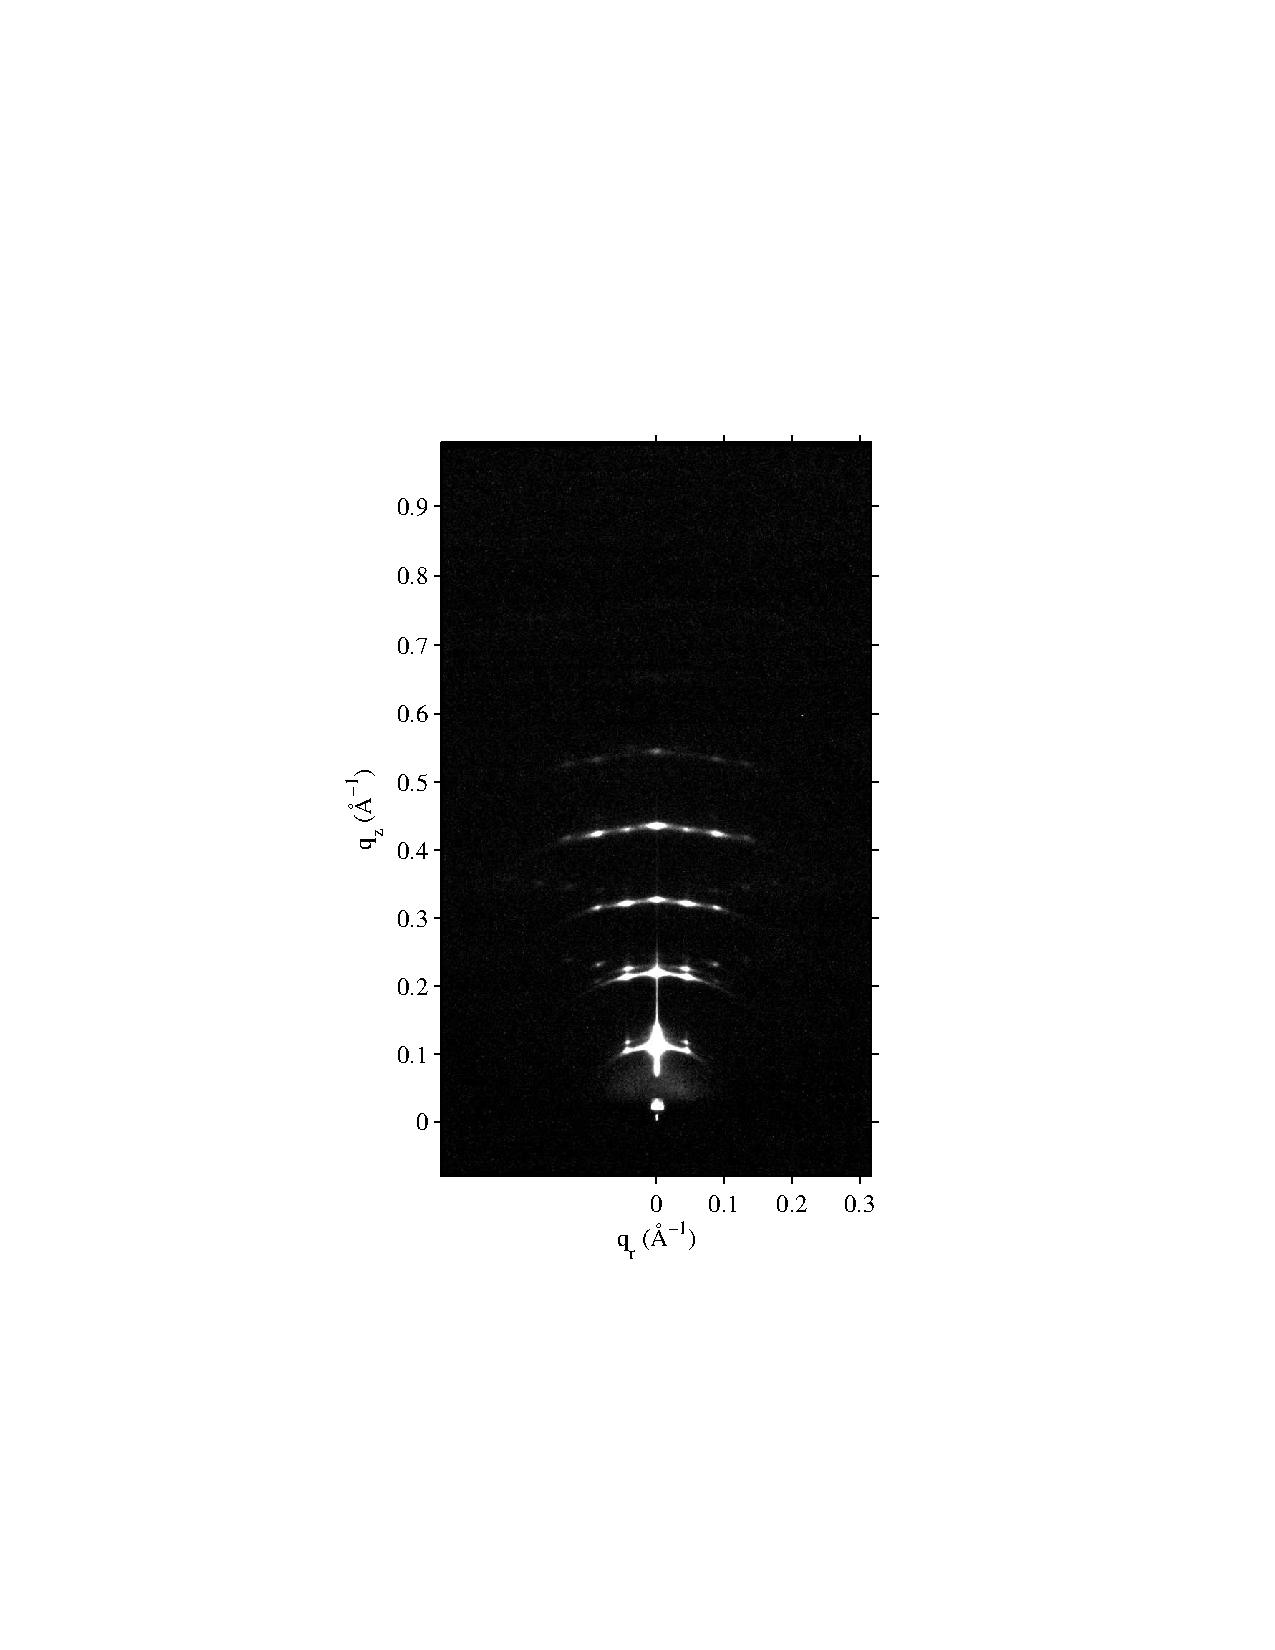
\includegraphics[trim=160 180 160 180,clip,width=0.49\textwidth]{figures/ripple/ripple083}
  %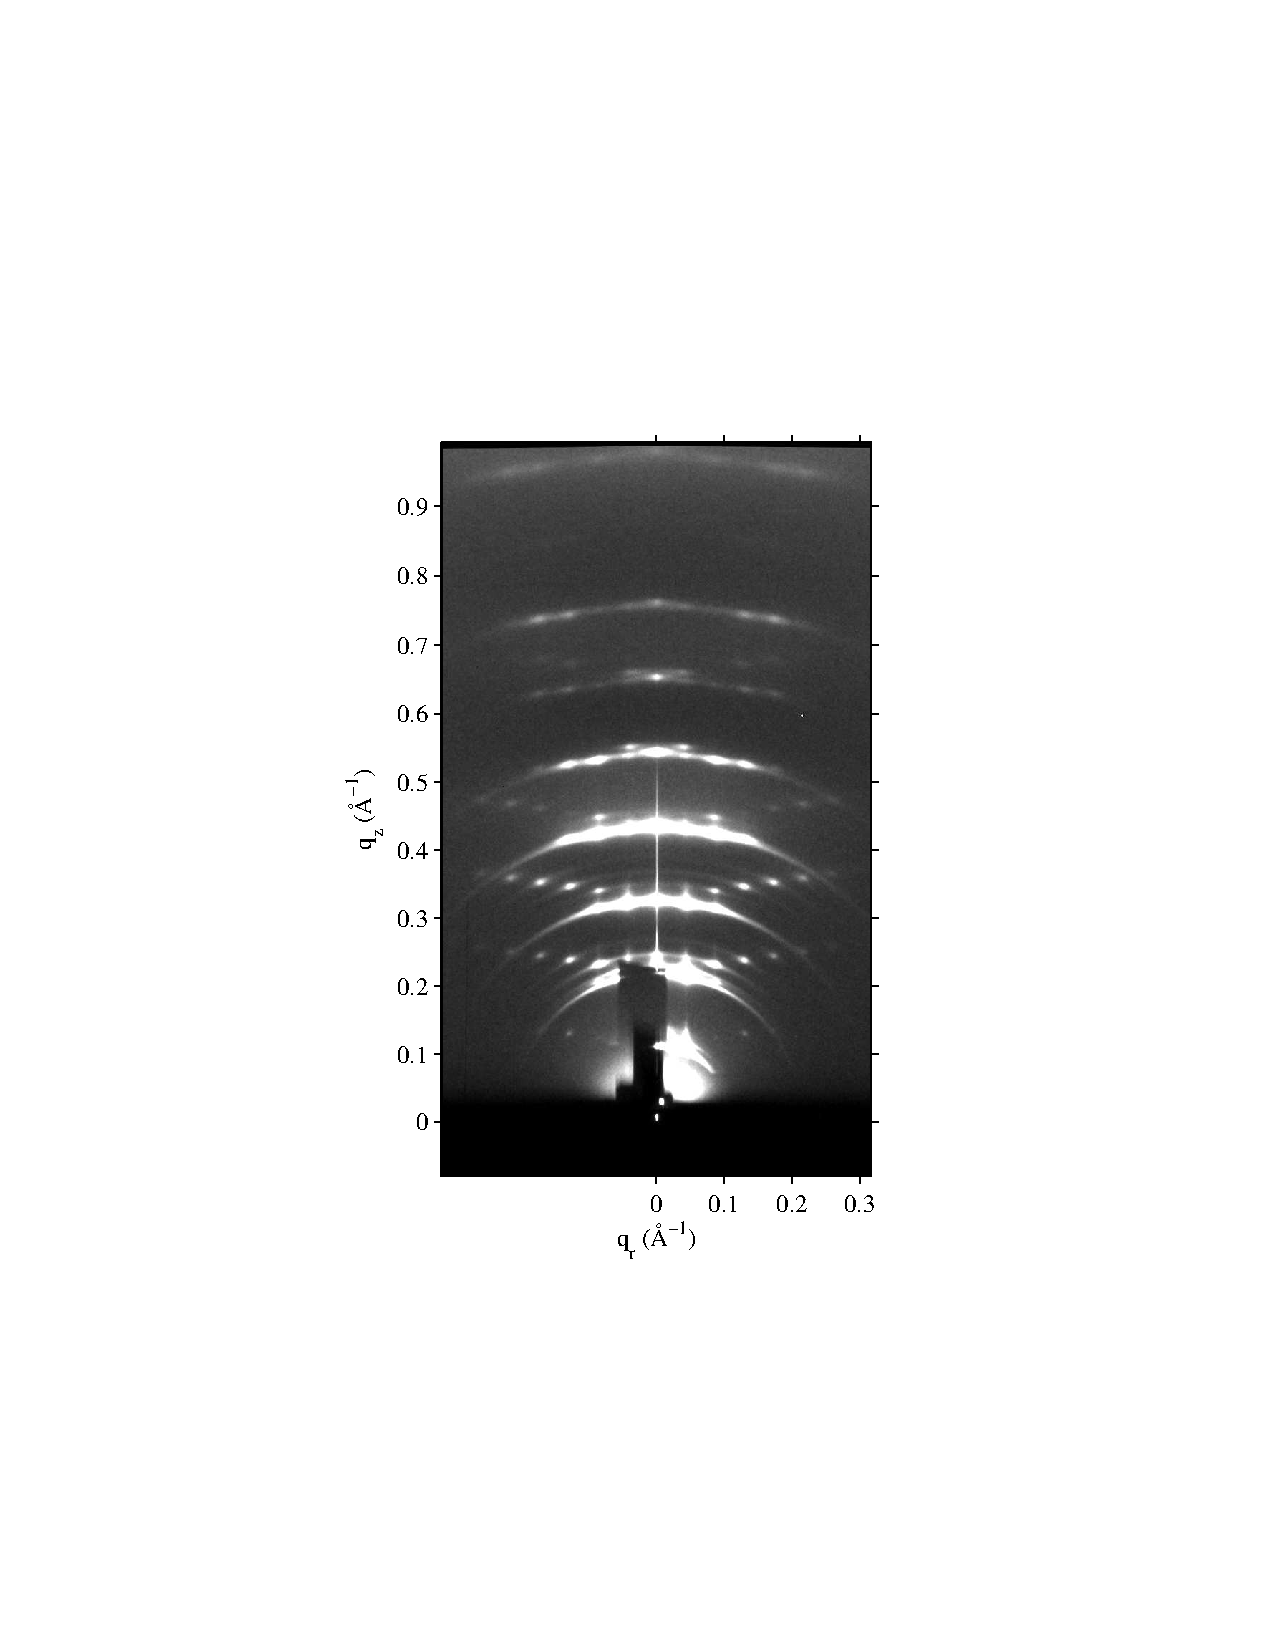
\includegraphics[trim=160 180 160 180,clip,width=0.49\textwidth]{figures/ripple/ripple085}
  \caption{1 second exposure (left) and 60 second exposure (right) of the low
  angle X-ray scattering from the DMPC ripple phase in gray log scales. 
  The index $h$ is 
  labeled in green. $(3,k)$ reflections are identified in cyan. 
  The shadow cast by 100 $\mu$m thick molybdenum attenuator blocking
  strong (1,0) and (2,0) orders in the right image is labeled as attenuator
  and extends from $q_z$ = 0 \AA$^{-1}$ to 0.2 \AA$^{-1}$.
  $D$ = 57.8 \AA, $\lambda_r$ = 145.0 \AA, and $\gamma$ = 97.8\textdegree.}
  \label{fig:ripple_laxs_images}  
\end{figure} 

\begin{figure}[jtbp]
  \centering
  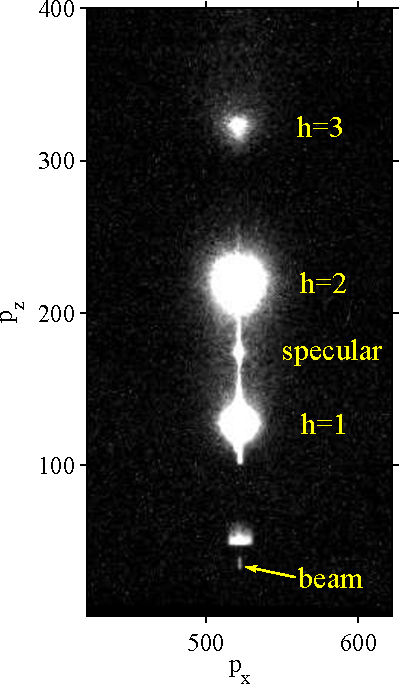
\includegraphics[width=0.45\textwidth]{figures/ripple/MMs/laxs/olddopc045_labels}
  \quad
  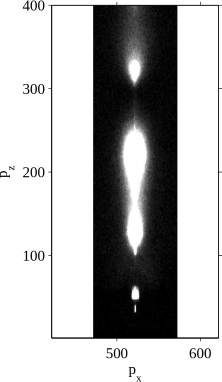
\includegraphics[width=0.45\textwidth]{figures/ripple/MMs/laxs/olddopc044}
  \caption{CCD images of X-ray scattering taken with (left) and without 
  (right) a nominally 25 $\mu$m thick Mo attenuator. These data were taken 
  at a fixed angle of incidence $\omega=0.8$\textdegree. The sample was an oriented film of 
  DOPC:DOPE (3:1) in the fluid phase at 37 \textcelsius. The wavelength
  was 1.175 \AA, the same as the one used for the ripple phase experiment.
  The same gray scale is used in both images. 100 pixel =  0.11 \AA$^{-1}$ in $q$. 
  A small dot located about $(p_x,p_z)=(520,170)$ between the first and second orders is 
  a specular reflection from the substrate. The exposure times were 1 second.}
  \label{fig:olddopc}
\end{figure}

\begin{figure}[htbp]
  \centering
  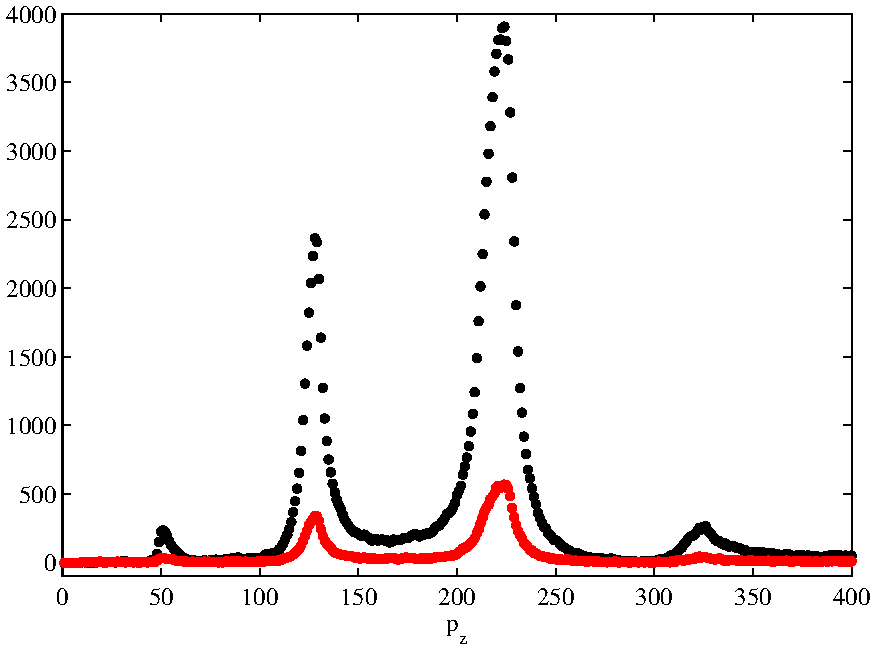
\includegraphics[width=0.45\textwidth]{figures/ripple/MMs/laxs/attenuator1}
  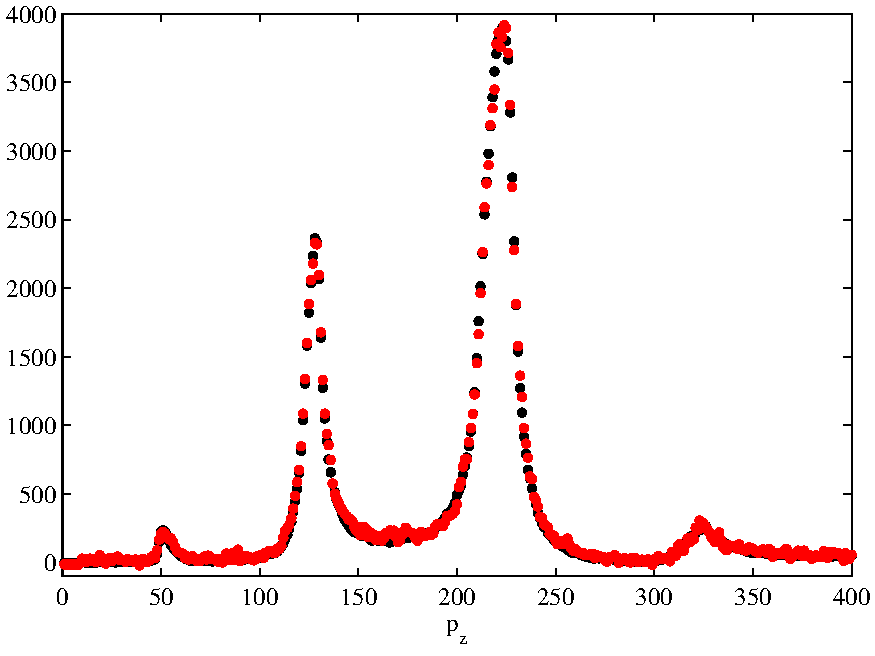
\includegraphics[width=0.45\textwidth]{figures/ripple/MMs/laxs/attenuator2}
  \caption{Vertical $p_z$ slices of X-ray images shown in Fig.~\ref{fig:olddopc}
  (left). The scattering intensity measured with the attenuator (red solid circles) 
  was multiplied by 
  a factor of 6.9 and compared to the intensity measured 
  without the attenuator (black solid circles, right).}
  \label{fig:attenuator}
\end{figure}

\subsection{Near Grazing Incidence Wide Angle X-ray Scattering Experiment}
\label{NGIWAXS_method}
The high resolution X-ray scattering experiment was also carried out at 
the G1 station. To achieve a higher instrumental resolution than that for 
the low angle X-ray scattering experiment described in a previous section, 
a (111) silicon monochromator was used, which gave $\Delta E/E$ of 0.01\%.
Due to the geometry of the G1 station, the Si monochromator was placed in
the G1 hutch, in series with the multilayer monochromator. 
The instrument was set up by the G1
station scientist, Author Woll, and the assistant scientist, Dr. Robin Baur.

The energy of the beam was 10.55 keV (wavelength = 1.175 \AA).
The horizontal and vertical divergence of the X-ray beam were
$4.2 \times 10^{-5}$ rad and $1.6 \times 10^{-4}$ rad, respectively. 
The horizontal beam width was 4 pixels (0.28 mm) as shown in
Fig.~\ref{fig:NGIWAXS_beam}.
With this beam, the scattering resolution in the wide angle region 
was dominated by the geometric broadening. The broadening was due to the
sample width along the beam direction and the horizontal beam width 
(Fig.~\ref{fig:geometric_broadening}. From the geometry of the experiment, 
the geometric broadening $\Delta x$ can be determined,
\[
\Delta x = \Delta x_\textrm{beam} + w_\textrm{s}\tan(2\theta).
\] 
The total scattering angle $2\theta$ for the ripple WAXS was approximately 
16\textdegree. 
To minimize the contribution from the sample, the sample was trimmed to 1 mm
along the beam direction. 
(edge effect)The width of 1 mm was chosen because (1) I could not trim more
without a more sophisticated device than a simple razor blade, (2) a very
narrow sample would be a weak scattering body, and (3) any effect from 
the sample edge might become too significant to ignore. 
Given the above reasons and due to limited availability
of synchrotron beam time, I considered a 1 mm width to be reasonable.
With these values, the resolution is $\Delta x = 0.57$ mm = 8 pixels, 
which would be the unresolved width of an intrinsically infinitely sharp wide angle peak.
The sample to detector distance were 220.6 mm, measured using silver behenate.
Then, the minimum peak width measured in $q$-space would be
$\Delta q \approx 0.014$ \AA$^{-1}$.
Wide angle X-ray scattering was collected at an incident angle of 0.2\textdegree. 
The total external reflection from an air-lipid interface occurs approximately 
at 0.1\textdegree\ and 0.17\textdegree for air-silicon interface, 
so 0.2\textdegree\ is not quite grazing incidence.
Grazing incidence usually implies that the incident angle is less than the 
critical angle for a total external reflection.
Therefore, 0.2\textdegree is called near grazing incidence in this thesis.

%S1L = 153.6 mm, S1H = 220.6 mm, and S2 = 359.7 mm

\begin{figure}[htbp]
  \centering
  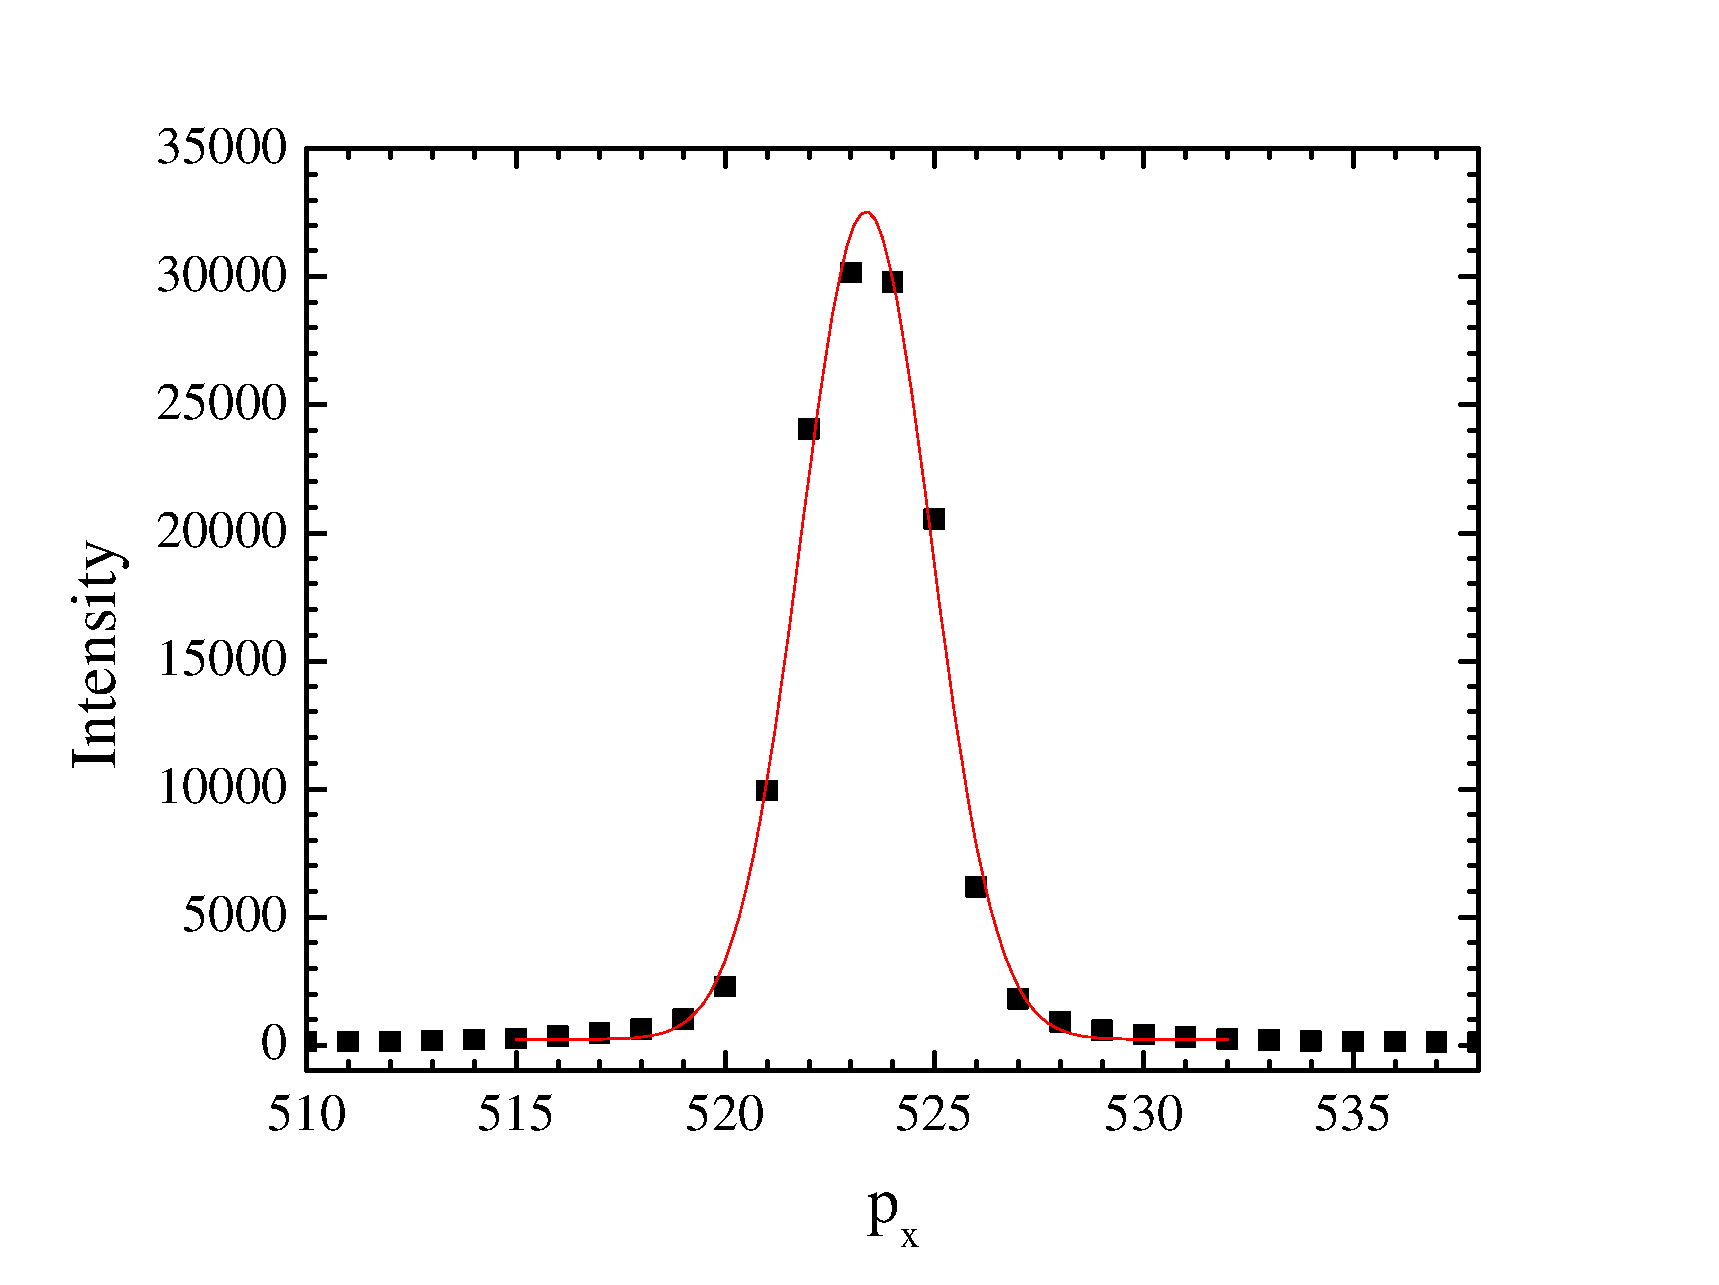
\includegraphics[width=0.7\textwidth]{figures/ripple/MMs/waxs/beamx_hr}
  \caption{The horizontal profile of the beam used in the high resolution 
  experiment. The CCD angular resolution $\Delta\theta$ = 0.0092\textdegree\,
  corresponding to $\Delta q$ = 0.0017 \AA$^{-1}$, at the sample to detector
  distance of 220.6 mm. The beam FWHM = 3.7 pixels = 0.26 mm, giving
  $\Delta\theta$ = 0.034\textdegree\ or $\Delta q$ = 0.0063 \AA$^{-1}$. }
  \label{fig:NGIWAXS_beamx}
\end{figure} 

\begin{figure}[htbp]
  \centering
  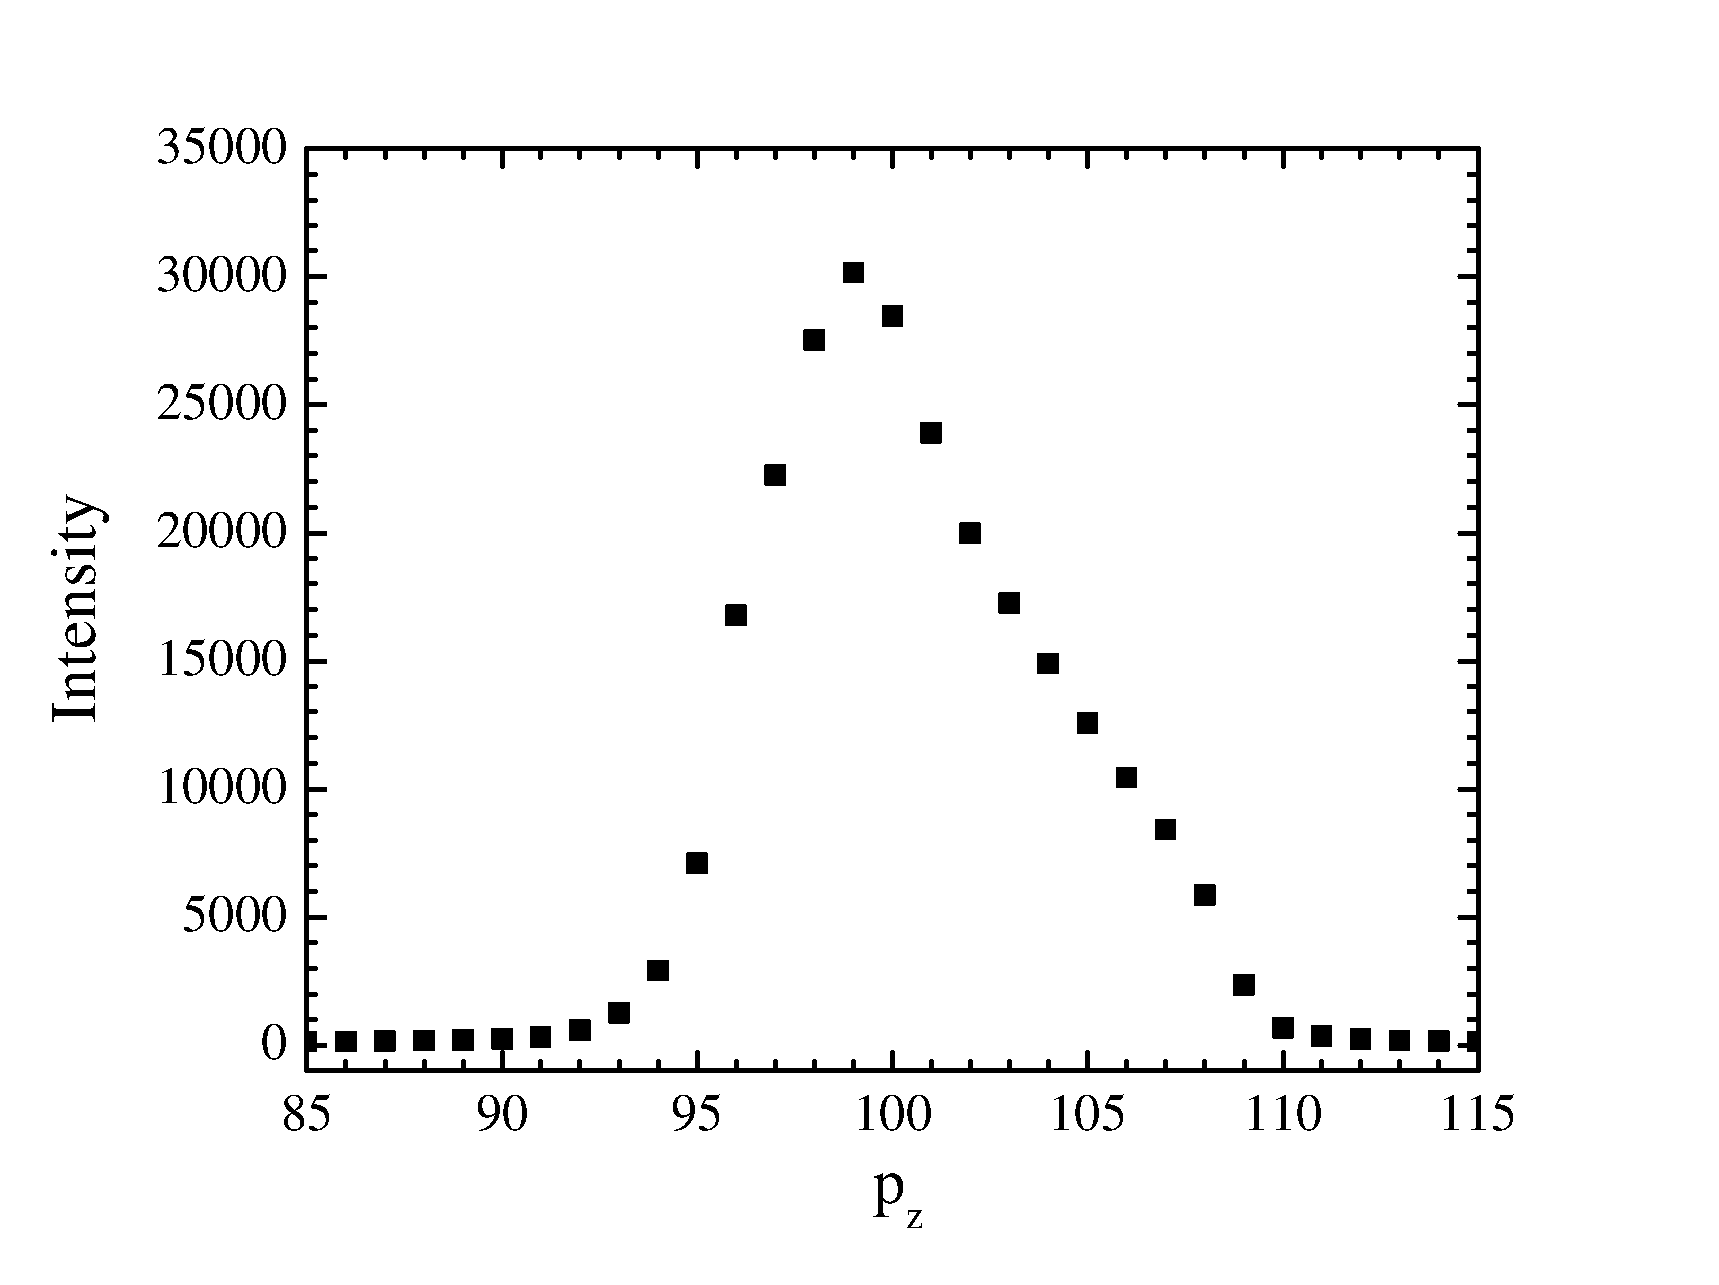
\includegraphics[width=0.7\textwidth]{figures/ripple/MMs/waxs/beamz_hr}
  \caption{The vertical profile of the beam used in the high resolution experiment.
  The beam height = 9 pixels = 0.64 mm.}
  \label{fig:NGIWAXS_beamz}
\end{figure} 

\begin{figure}[htbp]
  \centering
  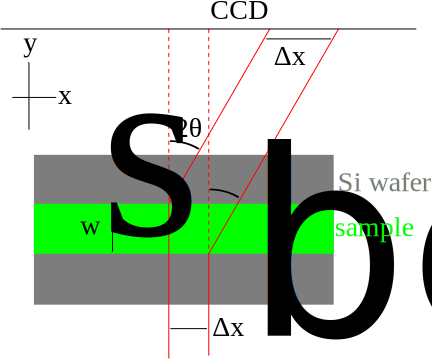
\includegraphics[width=0.5\textwidth]{figures/ripple/MMs/waxs/geometric_broadening}
  \caption{In-plane geometric broadening due to the sample width $w_s$ and the beam width $\Delta x_\textrm{beam}$.
  A top view of the sample (green) on the Si wafer (gray) and the
  incoming and diffracted X-rays (bounded by red solid lines)
  are shown. The total in-plane scattering
  angle for a lipid chain-chain correlation is labeled as $2\theta$, and 
  the geometric broadening as $\Delta x$.}
  \label{fig:geometric_broadening}
\end{figure}

\subsection{Transmission Wide Angle X-ray Scattering Experiment}
\label{TWAXS_method}
The transmission wide angle X-ray scattering (TWAXS) experiment was also 
carried out at the G1 station, and a similar instrumental resolution
to the one in Sec.~\ref{sec:LAXS_method} was used.
The sample to detector distance was measured to be 170 mm using sliver behenate 
when the angle of incidence $\omega$ was 0\textdegree.
The incident angle was set to -45\textdegree\ for transmission data
collection. A 35 $\mu$m thick silicon substrate absorbs an X-ray at
10.5 keV by 20\%\ \cite{ref:cxro}. 
To measure a D-spacing, mosaic spread of the sample was exploited. 
Unfortunately,
the axis of the rotation motor did not coincide with the sample axis, so
the sample to detector distance varied as $\omega$ was varied. To accurately
measure the sample to detector distance, low angle scattering was collected
at a fixed $\omega$. Due to the sample mosaic spread, many orders were
visible. While the relative intensity of each order was inaccurate, 
the position of peaks was the same as that observed with a rotating sample.
The sample to detector distance was accurately measured at $\omega$ = 0\textdegree\
using a silver behenate sample. From the geometry of the sample holder,
a shift in the sample to detector distance was estimated for an arbitrary 
incident angle $\omega$.

Explain how we estimated the sample to detector distance at
$\omega$ = -45\textdegree. Explain how we leveled the sample 
(using the sample scattering and ascan).
The background scattering was collected by replacing the sample with a bare 
wafer.

\begin{figure}[htbp]
  \centering
  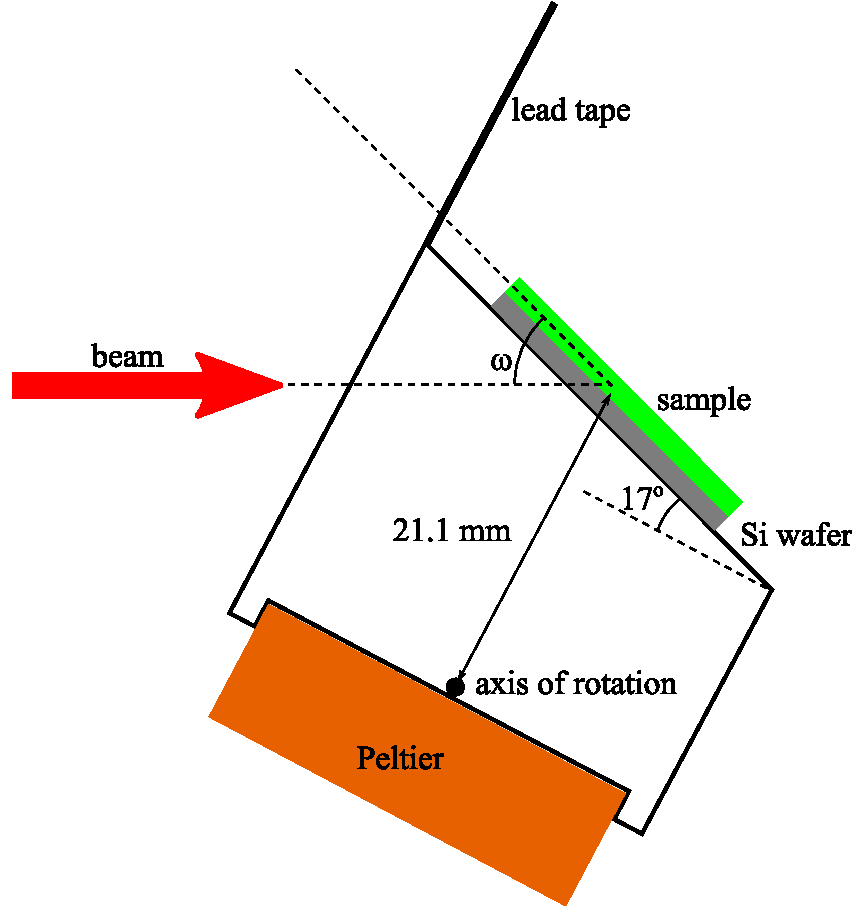
\includegraphics[width=0.55\textwidth]{figures/ripple/MMs/transmission/holder_side}
  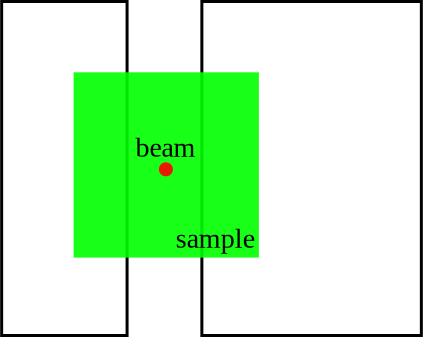
\includegraphics[width=0.35\textwidth]{figures/ripple/MMs/transmission/holder_top}
  \caption{Schematics of the sample holder in the transmission mode.
  Side (left) and top (right) views are shown. The thickness of the Si wafer
  = 35 $\mu$m. The thickness of the sample $\approx$ 10 $\mu$m. The
  distance between the axis of rotation and sample = 21.1 mm.}
  \label{fig:holder_schematic}
\end{figure}

\begin{figure}[htbp]
  \centering
  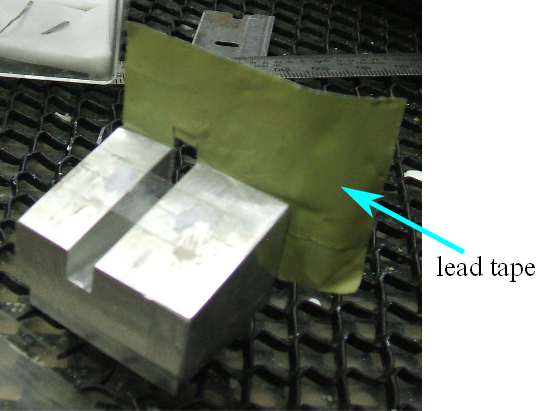
\includegraphics[width=0.45\textwidth]{figures/ripple/MMs/transmission/sample_holder1}
  \caption{Picture of the sample holder looking from above. A lead tape was
  attached to the back of the sample holder to help reduce the background 
  scattering, typically coming from the air gap between the flightpath snout
  and the mylar window of the chamber.}
  \label{fig:holder_picture}
\end{figure}

\begin{figure}[htbp]
  \centering
  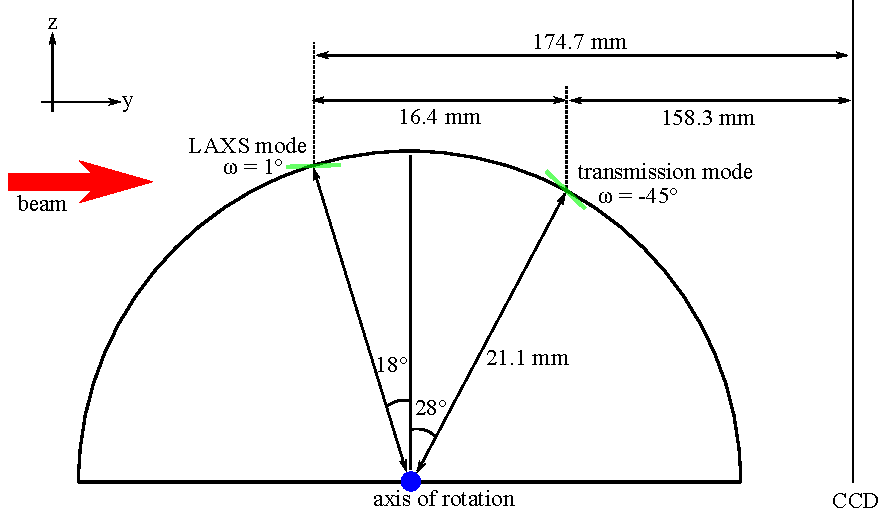
\includegraphics[width=0.8\textwidth]{figures/ripple/MMs/transmission/sgeometry}
  \caption{Circular path followed by the sample 
  as the angle of incidence $\omega$ was changed. The sample to detector distance and 
  $D$-spacing of the sample were measured in the LAXS mode, where $\omega$ = 1\textdegree. WAXS images
  were collected at the transmission mode, where $\omega$ = -45\textdegree. 
  The $z$ position of the sample was
  slightly higher at the LAXS mode than at the transmission mode, so the 
  sample holder was vertically shifted for different modes.}
  \label{fig:sgeometry}
\end{figure}



\begin{figure}[htbp]
  \centering
  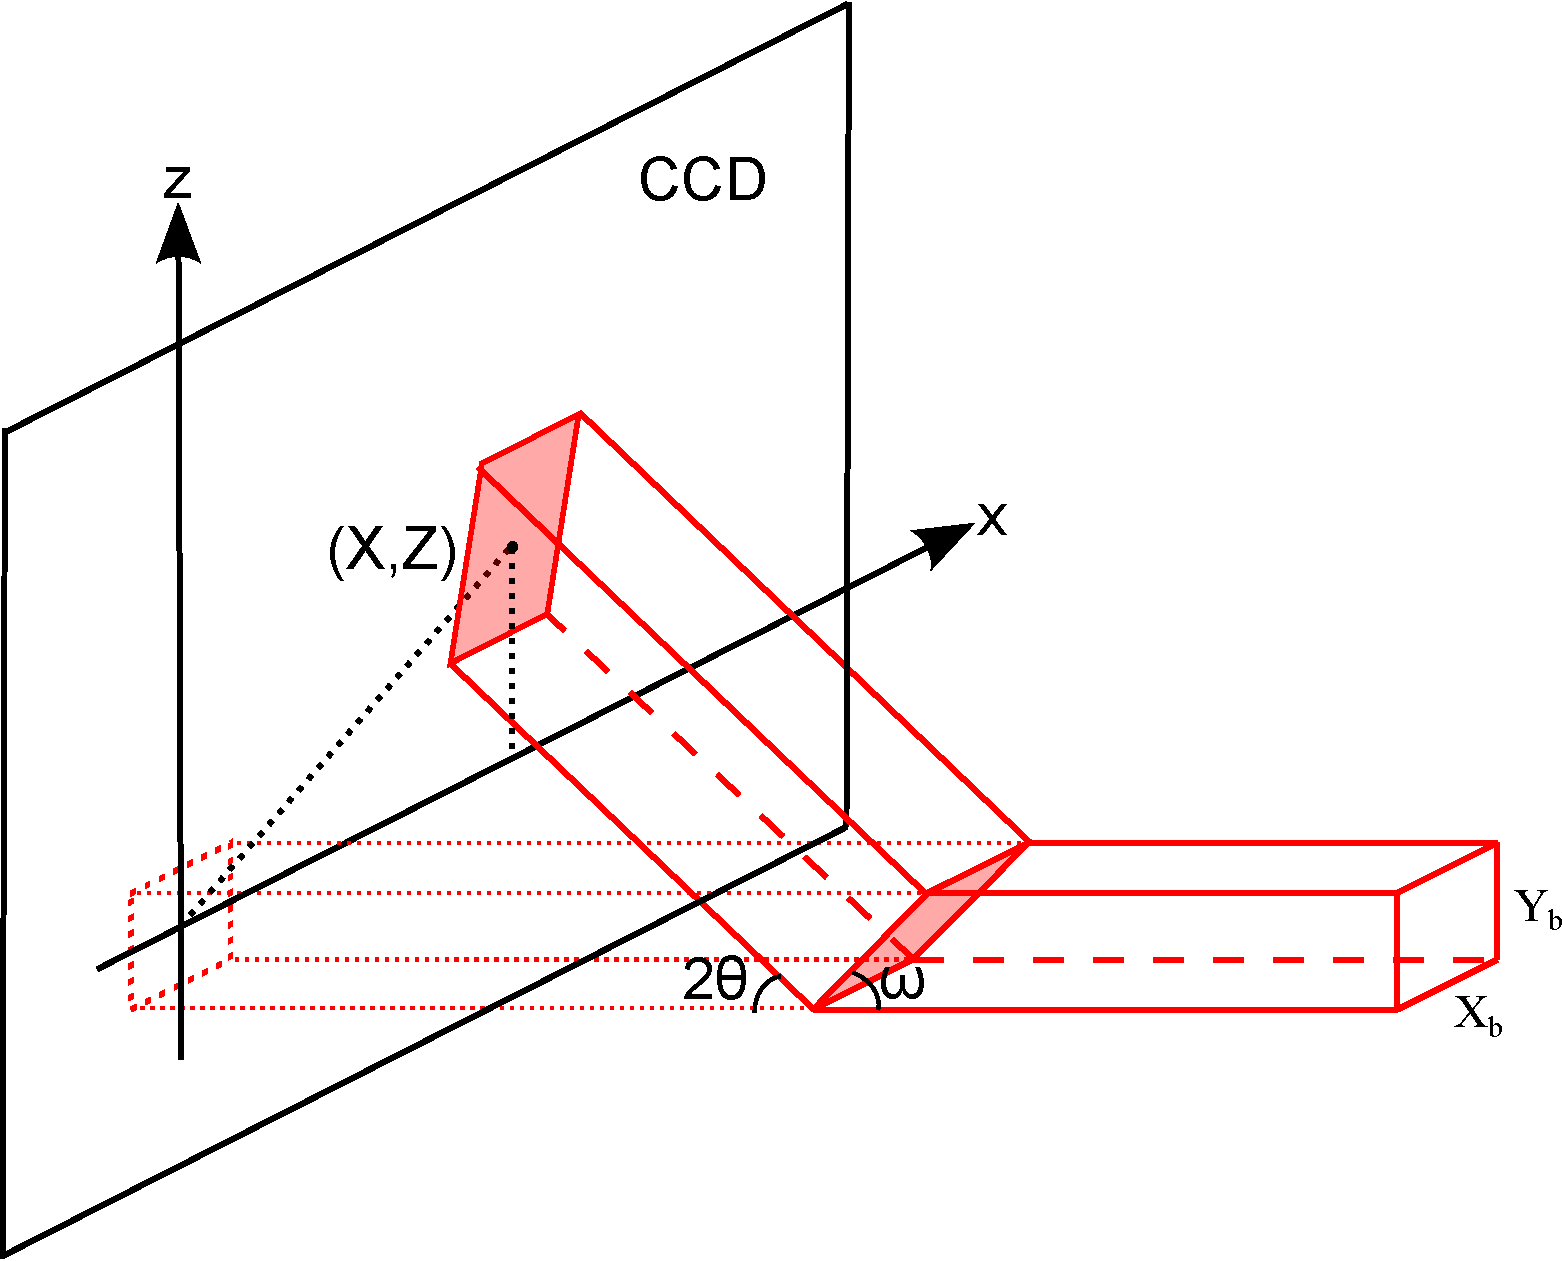
\includegraphics[width=0.5\textwidth]{figures/ripple/MMs/transmission/geometric_broadening1}
  \caption{Geometric broadening in TWAXS. The cross section of the incoming X-ray 
  with the sample and the CCD detector are both shaded in red.}
  \label{fig:gb_trans1}
\end{figure}

\begin{figure}[htbp]
  \centering
  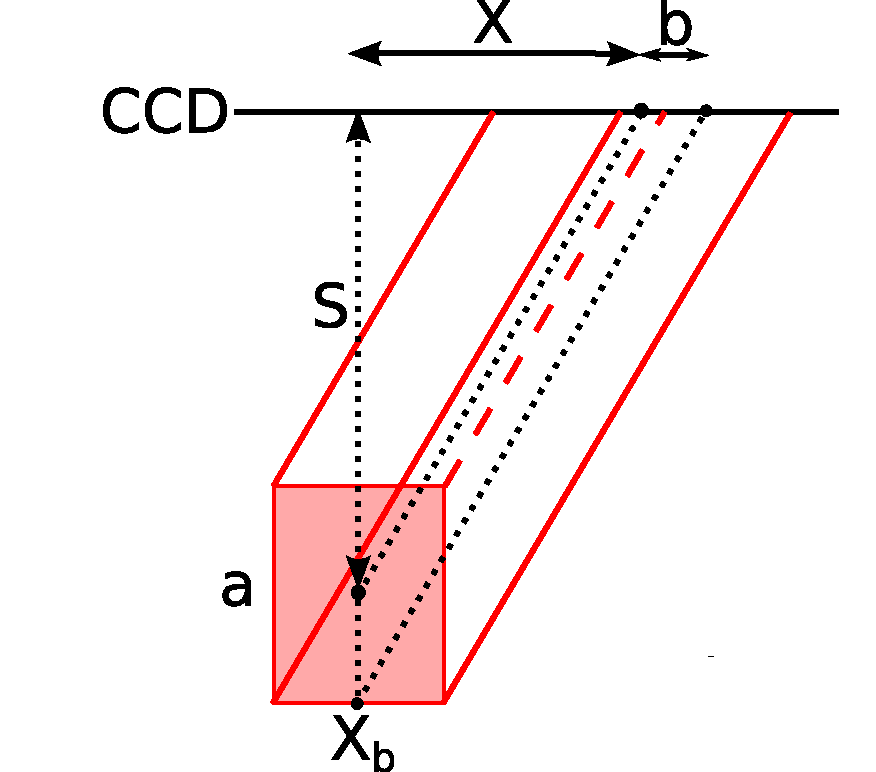
\includegraphics[width=0.5\textwidth]{figures/ripple/MMs/transmission/geometric_broadening2}
  \caption{Top view of geometric broadening in TWAXS. The cross section of the incoming X-ray 
  with the sample is shaded in red.}
  \label{fig:gb_trans2}
\end{figure}

\begin{figure}[htbp]
  \centering
  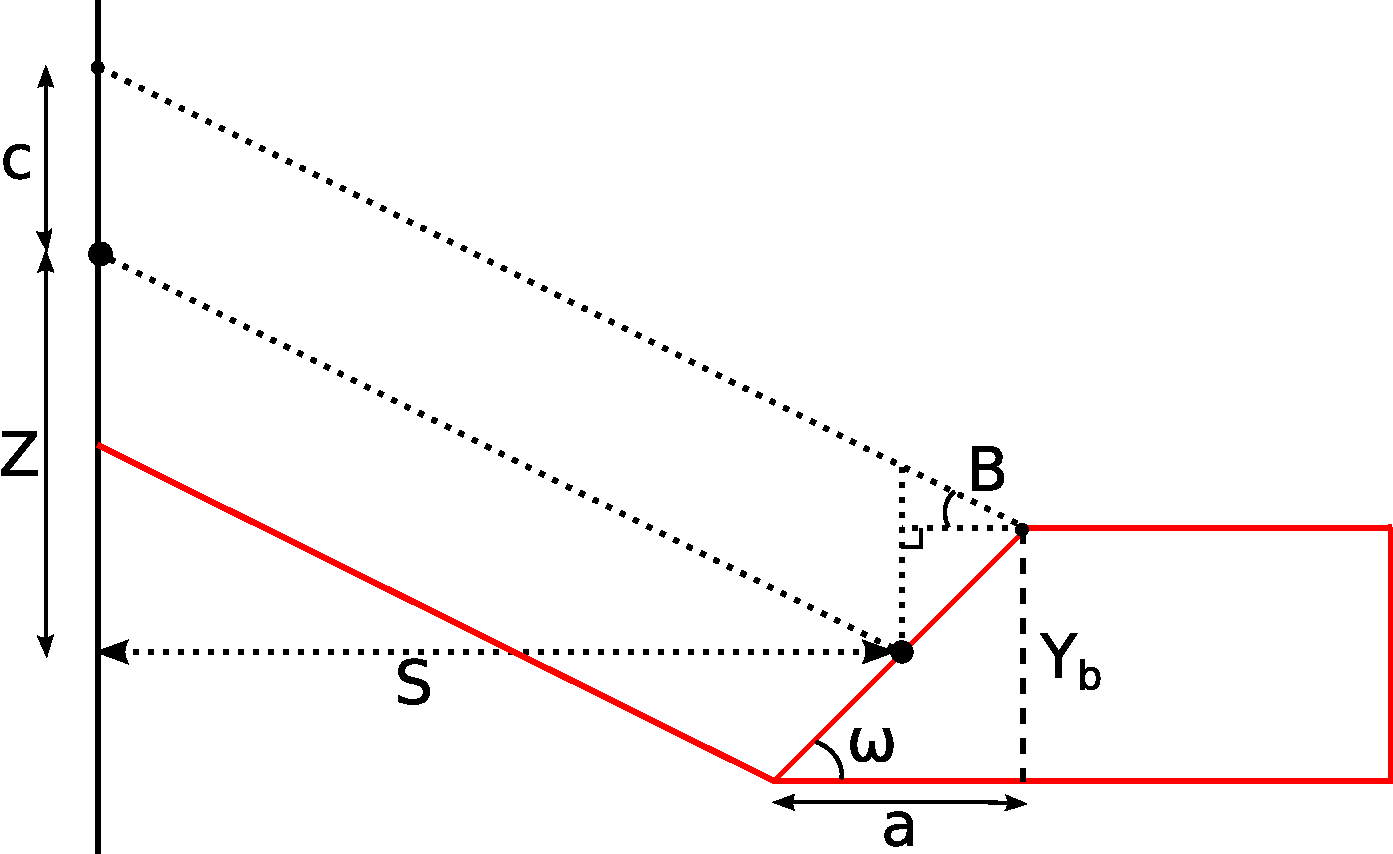
\includegraphics[width=0.5\textwidth]{figures/ripple/MMs/transmission/geometric_broadening3}
  \caption{Side view of geometric broadening in TWAXS. The cross section of the outgoing X-ray 
  with the CCD detector is shaded in red.}
  \label{fig:gb_trans3}
\end{figure}

\begin{figure}[htbp]
  \centering
  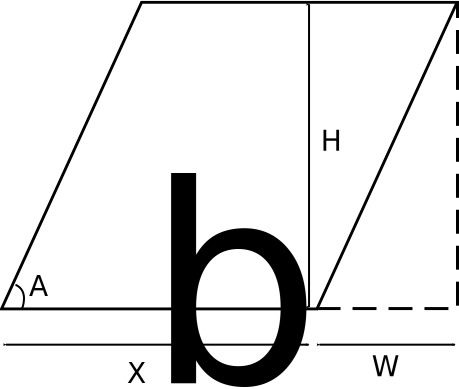
\includegraphics[width=0.3\textwidth]{figures/ripple/MMs/transmission/geometric_broadening4}
  \caption{Projection of rectangular beam on the detector.}
  \label{fig:gb_trans4}
\end{figure}

%%%%%%%%%%%%%%%%%%%%%%%%%%%%%%%%%%%%%%%%%%%%%%%%%%%%%%%%%%%%%%%%%%%%%%%%%%%%%%%
\newpage
\section{LAXS: analysis}
\subsection{Lattice Structure}\label{sec:lattice_structure}
The unit cell vectors for the two-dimensional oblique lattice shown in Fig.~\ref{fig:unit_cell}
can be expressed as 
\begin{equation}
  \mathbf{a} = \frac{D}{\tan\gamma}\xhat + D\zhat
\end{equation}
and
\begin{equation}
  \mathbf{b} = \lambda_r\xhat.
\end{equation}
The corresponding reciprocal lattice unit cell vectors are
\begin{equation}
  \mathbf{A} = \frac{2\pi}{D}\zhat
\end{equation}
and
\begin{equation}
  \mathbf{B} = \frac{2\pi}{\lambda_r}\xhat - \frac{2\pi}{\lambda_r\tan\gamma}\zhat.
\end{equation}
The reciprocal lattice vector, $\mathbf{q}_{hk}$ for the Bragg peak with 
Miller indices $(h,k)$ is 
\begin{equation}
  \mathbf{q}_{hk}=h\mathbf{A}+k\mathbf{B},
\end{equation}
so its Cartesian components are
\begin{align}
  & \mathbf{q}_{hk}\cdot\xhat = q_{hk}^x = \frac{2\pi k}{\lambda_r} \equiv q_{k}^x \\
  & \mathbf{q}_{hk}\cdot\yhat = q_{hk}^y = 0 \\
  & \mathbf{q}_{hk}\cdot\zhat = \qz{hk} = \frac{2\pi h}{D} - \frac{2\pi k}{\lambda_r\tan\gamma}.
\end{align}
Our sample consists of many ripple domains with a uniform distribution of in-plane directions of the
ripple wave vector, $\mathbf{b}$ in Fig.~\ref{fig:unit_cell}. 
In this case, $q_{hk}^x$ and $q_{hk}^y$ are combined to 
give $q_{hk}^r = 2\pi k/\lambda_r$.

%%%%%%%%%%%%%%%%%%%%%%%%%%%%%%%%%%%%%%%%%%%%%%%%%%%%%%%%%%%%%%%%%%%%%%%%%%%%%%%
\subsection{Sample q-space}\label{sec:sample_q-space}
The incoming and outgoing wavevectors of the x-ray beam in Fig.~\ref{fig:laxs_setup}
are given by
\begin{equation}
  \kin = \frac{2\pi}{\lambda} \yhat, \quad
  \kout = 
    \frac{2\pi}{\lambda} \left( 
      \sin 2\theta \cos\phi \, \xhat
      + \cos 2\theta \, \yhat
      + \sin 2\theta \sin\phi \, \zhat 
    \right),
  %\label{eq:kinkout}
\end{equation}
where $\lambda$ is the wavelength of x-ray, $2\theta$ is the total scattering
angle, and $\phi$ is the angle measured from the equator on the detector. 
The scattering vector (also called
momentum transfer vector) is
the difference between $\kin$ and $\kout$,
\begin{align}
  \mathbf{q} &= \kout - \kin \nonumber \\
             &= q \left( 
                  \cos\theta\cos\phi \, \xhat - \sin\theta \, \yhat
                  + \cos\theta\sin\phi \, \zhat
                \right),
  \label{eq:q_vector}
\end{align}
where $q=4\pi\sin\theta/\lambda$ is the magnitude of the scattering vector. 
When the sample is rotated by $\omega$ about the lab x-axis in the clockwise 
direction as shown in Fig.~\ref{fig:laxs_setup}, the sample $q$-space also rotates and 
are given by  
\begin{equation}
  \mathbf{\hat{e}_x} = \xhat, \quad
  \mathbf{\hat{e}_y} = \cos\omega\,\yhat + \sin\omega\,\zhat, \quad
  \mathbf{\hat{e}_z} = -\sin\omega\,\yhat + \cos\omega\,\zhat.
  \label{eq:smp_coord}
\end{equation}
From Eq.~(\ref{eq:q_vector}) and (\ref{eq:smp_coord}), we find Cartesian
components of the sample $q$-space to be
\begin{align}
  q_x &= \mathbf{q}\cdot\mathbf{\hat{e}_x} 
       = q\cos\theta\cos\phi, 
       \nonumber\\
  q_y &= \mathbf{q}\cdot\mathbf{\hat{e}_y} 
       = q\left(-\sin\theta\cos\omega + \cos\theta\sin\phi\sin\omega\right), 
       \nonumber\\
  q_z &= \mathbf{q}\cdot\mathbf{\hat{e}_z} 
       = q\left(\sin\theta\sin\omega + \cos\theta\sin\phi\cos\omega\right).
       \label{eq:qxqyqz}
\end{align}
The position, $(X,Z)$, of a CCD pixel is measured with respect to the beam 
and given by
\begin{equation}
  X = S \tan 2\theta \cos\phi, \quad Z = S \tan 2\theta \sin\phi,
  \label{eq:XZ}
\end{equation} 
where $S$ is the distance between the sample and detector.

\begin{figure}[htbp]
  \centering
  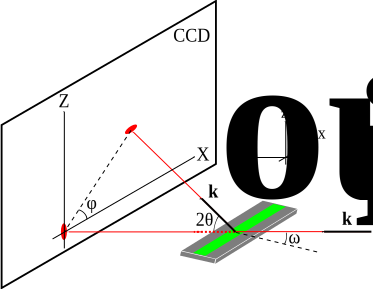
\includegraphics[width=0.8\textwidth]{figures/ripple/analysis/laxs_setup}
  \caption{Experimental reflectivity geometry.}
  \label{fig:laxs_setup}
\end{figure}

From a model for the electron density of a lipid bilayer, one calculates
the X-ray scattering intensity pattern, $I(\mathbf{q})$. Then, Eq.~(\ref{eq:qxqyqz})
and (\ref{eq:XZ}) relate $I(\mathbf{q})$ to the experimentally measured
intensity pattern, $I(X,Z)$. It is important to remember that a given pixel
position, $(X,Z)$, corresponds to a triplet $(q_x, q_y, q_z)$. Fully exploring 
the sample $q$-space requires changing $\omega$ for a fixed wavelength, which was
achieved by continuously rotating the sample with a motor. In the ripple phase, 
because our sample has in-plane rotational symmetry,
the ripple side peaks ($h,k\neq 0$) make up Bragg rings while the main peaks ($h,k=0$) are still 
delta function like (see Fig.~\ref{fig:ripple_sample_qspace}) in $q$-space. In order for the main peak to be
observed, $\omega$ must be equal to $\theta_\mathrm{B}$, but the side peaks
are observed at any $\omega$. Those side peaks get slightly smeared due to 
integration over $q_y$.

For low angle x-ray scattering (LAXS), it is convenient to linearize the above
equations in terms of $\theta$ and $\omega$. In the small angle approximation, 
$\sin\phi \approx Z/(2S\theta)$ and $\cos\phi \approx X/(2S\theta)$, and
\begin{align}
  q_x &\approx \frac{4\pi\theta\cos\phi}{\lambda} \approx kX/S \nonumber\\
  q_y &\approx q_z\omega -\frac{4\pi\theta^2}{\lambda} \approx q_z\omega - \frac{\lambda q_z^2}{4\pi}\nonumber\\
  q_z &\approx \frac{4\pi\theta\sin\phi}{\lambda} \approx kZ/S,
  \label{eq:qxqyqz_small}
\end{align}
with $k=2\pi/\lambda$. For wide angle X-ray scattering, the exact relations given
by Eq.~(\ref{eq:qxqyqz}) are necessary. Especially in the transmission experiment,
where $\omega$ is large, an observed X-ray pattern appears nontrivial and becomes
almost impossible to analyze without the use of Eq.~(\ref{eq:qxqyqz}).
The transmission experiment is discussed in Sec.\ref{sec:TWAXS_results}.

\begin{figure}[htbp]
  \centering
  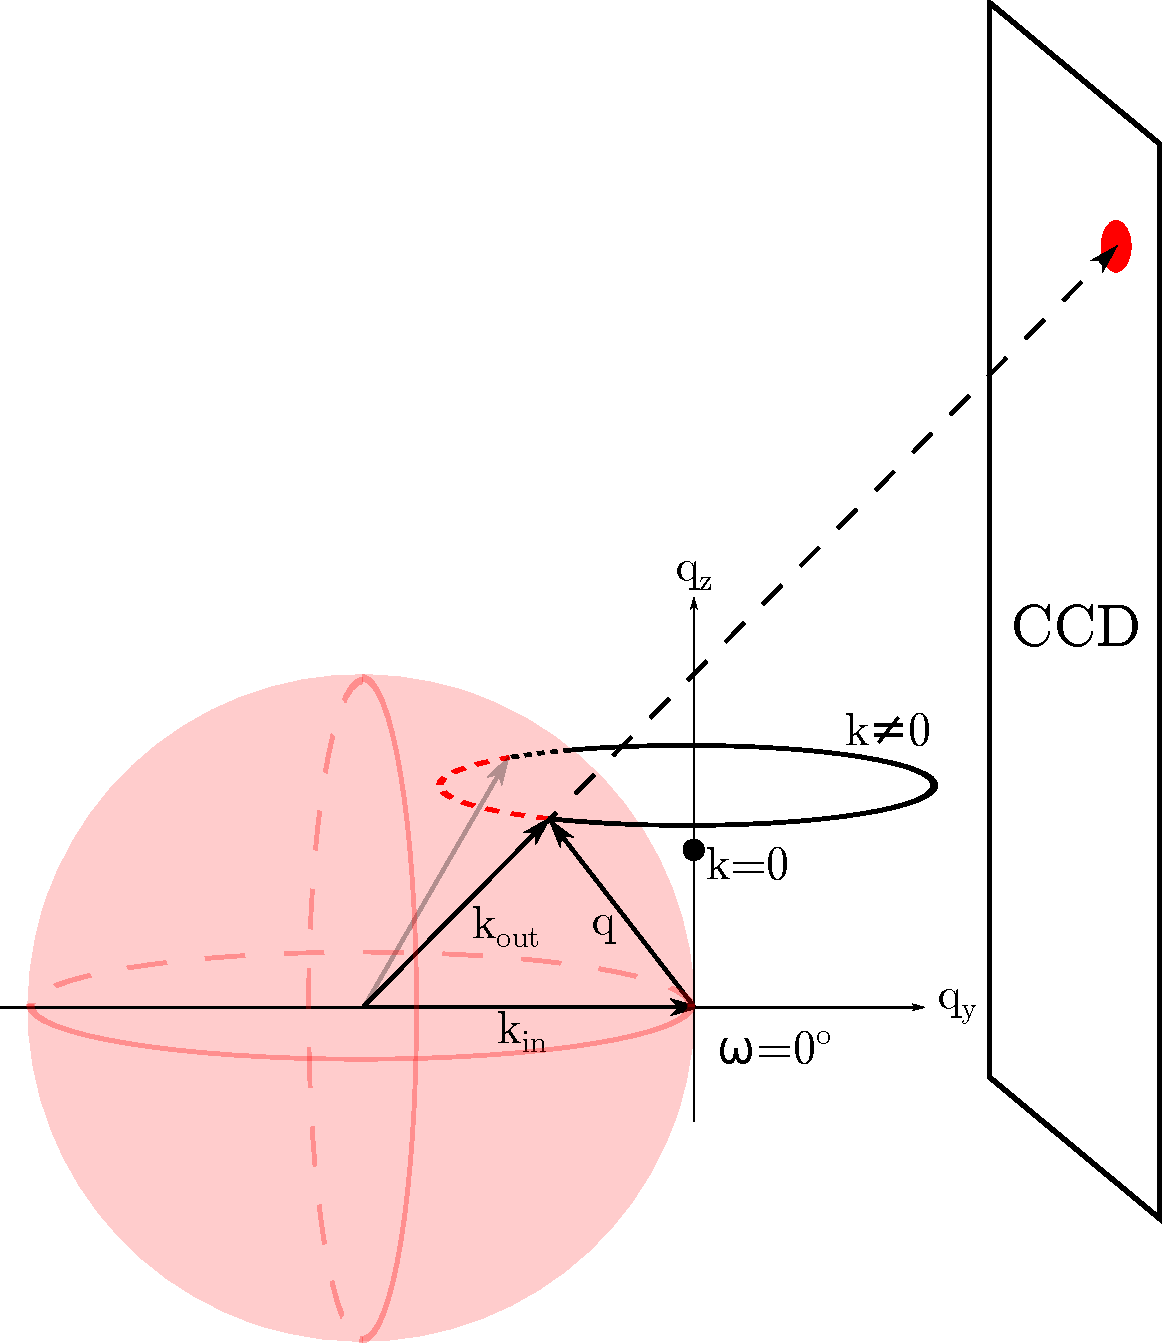
\includegraphics[width=0.8\textwidth]{figures/ripple/analysis/ripple_sample_qspace}
  \caption{Ewald sphere construction for the ripple phase diffraction in
  the low angle regime. A ripple $k=0$ peak is the solid, black circle
  on the $q_z$-axis.
  A ripple $k\neq 0$ ring is the black ring centered about the $q_z$-axis. 
  The portion of the ring that is 
  inside the Ewald sphere is shown as a red dashed line and the portion of the 
  ring that is outside but behind the Ew here to sayald sphere is shown as a black
  dotted line. The magnitude of the total scattering angle is exaggerated. 
  With a wavelength
  of 1.175 \AA, the magnitude $|\kin|=5.35$ \AA$^{-1}$. For a $h=5$ peak,
  $\qz{50}=0.54$ \AA$^{-1}$, one tenth of $k_\textrm{in}$.}
  \label{fig:ripple_sample_qspace}
\end{figure}

%%%%%%%%%%%%%%%%%%%%%%%%%%%%%%%%%%%%%%%%%%%%%%%%%%%%%%%%%%%%%%%%%%%%%%%%%%%%%%%
\subsection{Lorentz Correction}\label{sec:Lorentz_correction}
Our sample has in-plane rotational symmetry about the $z$-axis. 
Ignoring mosaic spread to which we will come back later, this means that the sample 
consists of many domains with differing ripple directions, all domains
being parallel to the substrate.  
In sample $q$-space, ripple ($h,k\neq 0$) side peaks are represented as rings 
centered at the meridian, or $q_z$-axis, 
while ($h,k=0$) main peaks are still points on the meridian 
(see Fig.~\ref{fig:ripple_sample_qspace}). 
Then, for an arbitrary incident angle $\omega$, $(h,0)$ peaks are not observed
while side peaks are observed for a range of $\omega$ as will now be explained. 

In order to capture all ($h,k$) peaks in one X-ray exposure, 
the sample was continuously rotated over a range of $\omega$, $\Delta\omega$,
about the $x$-axis. As a result of this rotation, 
the $(h,0)$ main peaks become arcs that subtend an angle $\Delta\omega$,
as shown in Fig.~\ref{fig:ewald_main}, with its length
equal to $\Delta\omega\qz{h0}$. 
The detector records the intersections of these arcs with the 
Ewald sphere, so the intrinsic scattering intensity of the $(h,k=0)$ reflections
is the product of the observed intensity, $\Io{hk}$ with the arc length, that is, 
\begin{equation}
  I_{h0} = \Delta\omega\qz{h0} \Io{h0}. \label{eq:main_ewald}
\end{equation}
This is the usual Lorentz correction for lamellar orders.

Now, we consider relative intensity of side peaks for a given order $h$.
As described earlier, $(h,k\neq 0)$ side peaks are represented as
rings whose radius is $\qr{hk}$ in the sample $q$-space. 
Because only the domains with the right ripple direction can satisfy the Bragg's condition at a given fixed
angle $\omega$, the intrinsic scattering intensity in this ring is reduced by 
a factor of $2\pi \qr{k}$ compared to the $(h,0)$ reflections.
This reduction of intensity can be nicely visualized by the Ewald sphere construction
shown in Fig.~\ref{fig:ripple_sample_qspace},
which shows that the entire rings are not intersected by the Ewald sphere at 
a fixed angle. Then, the intrinsic scattering intensity in a ring is
\begin{equation}
  I_{hk\neq 0} \propto 2\pi \qr{hk} \Io{hk}. \label{eq:side_ewald}
\end{equation}
During an X-ray exposure, the sample $q$-space rotates and 
the rings are intersected by the Ewald sphere at all our experimental incident angles $\omega$.
However, as Fig.~\ref{fig:ewald_side} shows, only small parts of the rings
are actually intersected with the Ewald sphere.  
To obtain the full expression for $(h,k\neq 0)$ reflections, we now turn
to a more rigorous calculation.

%Inverting Eq.~(\ref{eq:main_ewald}) and (\ref{eq:side_ewald}) 
%and realizing that the intensity is the form factor
%squared, we can calculate the observed intensity, $\Io{hk}$, 
%from a model for an electron density in the ripple phase.
%But above is not the whole story and we need to do more work.

%------------------------------------------------------------------------------
\begin{figure}[htbp]
  \centering
  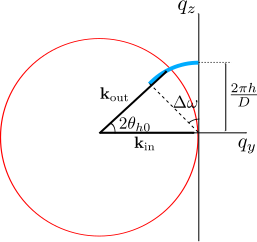
\includegraphics[width=0.45\textwidth]{figures/ripple/analysis/ewald_main}
  \caption{Side view of an arc of $k=0$ peak shown as a thick blue line.}
  \label{fig:ewald_main}
\end{figure}

\begin{figure}[htbp]
  \centering
  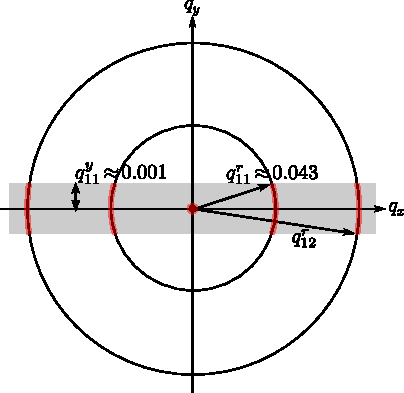
\includegraphics[width=0.45\textwidth]{figures/ripple/analysis/ewald_side_h1_ver1}
  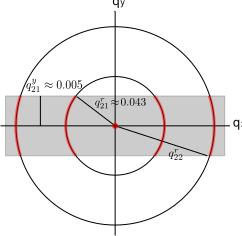
\includegraphics[width=0.45\textwidth]{figures/ripple/analysis/ewald_side_h2_ver1}
  \caption{$q$-space representations of Bragg peaks and Bragg rings 
  for $h=1 and 2$ and $k$ = 0, 1, and 2 in $\qz{hk}$ planes.
  The intersection between the Ewald sphere and 
  a Bragg peak/ring is indicated in red. 
  The observed intensity for the $k\neq 0$ orders is proportional to
  the fraction of the length of red arcs in the circumference. This 
  fraction is equal to one for $k=0$ reflections.
  Because the reflections are not in the same $q_z$ plane, the range of $q_y$ 
  integration indicated by the height of the gray rectangle is different for different
  $h$ orders. For $\gamma\neq 90$\textdegree, the range of $q_y$ integration is
  slightly different for different $k$ reflections with the same $h$. 
  The values shown are for $D=58$ \AA, $\lambda_r=145$ \AA, $\gamma=90$\textdegree,
  and $\lambda=1.175$ \AA. The magnitude of curvature of arcs is exaggerated.}
  \label{fig:ewald_side}
\end{figure}
%------------------------------------------------------------------------------

Mathematically, the rotation is  
equivalent to an integration over $\omega$. In low angle X-ray scattering, 
$q_z$ is nearly constant at a given pixel as $\omega$ is changed, which can be seen from 
Eq.~(\ref{eq:qxqyqz_small}). As Eq.~(\ref{eq:qxqyqz_small}) shows, 
$\omega$ dependence appears only through $q_y$, 
so rotating the sample is realized by integrating over $q_y$;
formally, we write $d\omega=dq_y/q_z$.
To derive the integration limits on $q_y$, let us consider two cases: 
(1) When $\omega \leq 0$,
the incoming X-ray beam is blocked by the back of the substrate. This sets 
the lower limit of $\omega$ to 0. Plugging $\omega=0$ in Eq.~\ref{eq:qxqyqz_small}),
we find the lower limit of the $q_y$ integration to be $-\lambda q_z^2/(4\pi)$.
(2) When $\omega \geq 2\theta$, the substrate blocks 
the outgoing X-ray, so the maximum $\omega = 2\theta$. 
Within the small angle approximation, $q_z \approx 4\pi\theta/\lambda$. 
Then, the maximum $\omega$ can be expressed as $\lambda q_z/(2\pi)$.
Plugging this expression for $\omega$ in Eq.~(\ref{eq:qxqyqz_small}),
we find the upper limit of the $q_y$ integration to be $\lambda q_z^2/(4\pi)$.
Also integrating over the detector pixels $X$ and $Z$ to obtain integrated intensity, 
we write the observed intensity as
\begin{align}
  \Io{hk} 
    &\propto \int dX \int dZ \int \mathop{d\omega} I_{hk} \nonumber \\
    &\propto \int dq_x \int dq_z 
             \int_{-\frac{\lambda q_z^2}{4\pi}}^{\frac{\lambda q_z^2}{4\pi}} 
             \frac{dq_y}{q_z} 
             I_{hk}(\mathbf{q}),
  \label{eq:I_obs_general}
\end{align}
where $1/q_z$ factor in $q_y$ integration is the usual Lorentz polarization factor
in the small angle approximation. 

For a crystalline sample with in-plane rotational symmetry, the
structure factor of a ripple Bragg peak is  
\begin{equation}
  S_{hk}(\mathbf{q}) = S_{hk}(q_r,q_z) 
  = \frac{1}{2\pi q_r}\delta(q_r-\qr{hk})\delta(q_z-\qz{hk}),
\end{equation} 
where $\qr{hk}=2\pi |k|/\lambda_r$. Thus, the scattering pattern in the 
ripple phase is a 
collection of Bragg rings for $k\neq 0$ centered at the meridian and the 
Bragg peaks for $k=0$ located along the meridian.  
The scattering intensity is $I(\mathbf{q})=|F(\mathbf{q})|^2S(\mathbf{q})$,
where $F(\mathbf{q})$ is the form factor. After the $q_z$ integration,
the observed, integrated intensity of $(h,k)$ peak is proportional to
\begin{equation}
  \Io{hk} 
    \propto \frac{\lvert F_{hk} \rvert^2}{\qz{hk}} \int\mathop{dq_x} 
            \int_{-q_{hk}^{y0}}^{q_{hk}^{y0}}
            \mathop{dq_y} \frac{\delta(q_r-\qr{hk})}{2\pi q_r},
  \label{eq:obs_integration}
\end{equation}
where $q_{hk}^{y0} = \lambda (\qz{hk})^2/(4\pi)$.
For side peaks ($k \neq 0$), we have 
\begin{align}
  \int\mathop{dq_x} \int_{-q_{hk}^{y0}}^{q_{hk}^{y0}}\mathop{dq_y} \frac{\delta(q_r-\qr{hk})}{2\pi q_r}
  &\approx \int_{-q_{hk}^{y0}/\qr{hk}}^{q_{hk}^{y0}/\qr{hk}} \mathop{d\phi} 
          \int \mathop{dq_r} q_r\frac{\delta(q_r-\qr{hk})}{2\pi q_r} \nonumber\\
  &= \frac{q_{hk}^{y0}}{\pi \qr{hk}}. 
  \label{eq:side_integrand}
\end{align}
For main peaks ($k=0$), we have 
\begin{align}
  \int\mathop{dq_x} \int_{-q_{hk}^{y0}}^{q_{hk}^{y0}}\mathop{dq_y} \frac{\delta(q_r-\qr{hk})}{2\pi q_r}
  &= \int_0^{2\pi}\mathop{d\phi} \int\mathop{dq_r} q_r\frac{\delta(q_r-\qr{hk})}{2\pi q_r} \nonumber\\
  &= 1 
  \label{eq:main_integrand}
\end{align}
Using Eq.~(\ref{eq:obs_integration} -- \ref{eq:main_integrand}), 
we write the observed integrated intensity as
\begin{align}
  \Io{h0} &\propto \frac{|F_{h0}|^2}{\qz{h0}} \label{eq:main}\\
  \Io{hk} &\propto \frac{|F_{hk}|^2}{\qz{hk}} \frac{q_{hk}^{y0}}{\pi \qr{hk}}
    = |F_{hk}|^2 \frac{\lambda \qz{hk}}{2\pi}\frac{1}{2\pi \qr{hk}}
    = |F_{hk}|^2 \frac{2\theta_{hk}}{2\pi \qr{hk}}, \label{eq:side}
\end{align}
where $2\theta_{hk} = \lambda \qz{hk}/(2\pi)$ is the incident angle at which 
the outgoing X-ray for the peak $(h,k)$ is blocked by the substrate.
Eq.~(\ref{eq:main}) and (\ref{eq:side}) relate the form factor calculated from
a model to the experimentally observed intensity, and are partially
equivalent to Eq.~(\ref{eq:main_ewald}) and (\ref{eq:side_ewald}). 

In non-linear least squares fitting procedure, 
we fitted the observed integrated intensity to
the calculated intensity from a bilayer model using these Lorentz corrections. 
This is because we can determine experimental uncertainties
on observed intensity rather than the Lorentz-corrected form factors. 
We avoid propagating the uncertainties by fitting a model to observed intensity. 

%%%%%%%%%%%%%%%%%%%%%%%%%%%%%%%%%%%%%%%%%%%%%%%%%%%%%%%%%%%%%%%%%%%%%%%%%%%%%%%
\subsection{Absorption Correction for LAXS}\label{sec:abs_correction_LAXS}
In this section, we derive the absorption correction for an oriented sample. 
The calculation involves an explicit integration over the incident angle, 
$\omega$, which is necessitated by the sample rotation during an X-ray exposure. 
The procedure is to write down an absorption factor, $A(\omega,\theta)$, for a 
given scattering angle at a given incident angle, and
then integrate over $\omega$. We ignore $q_x$ dependence because the X-ray
path inside the sample is nearly within the $y$-$z$ plane for low angle
scattering. The correction for wide angle scattering is described in a later
section.

%------------------------------------------------------------------------------
\begin{figure}[htbp]
  \centering
  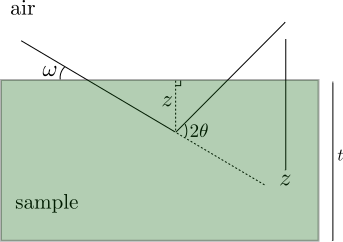
\includegraphics[width=0.5\textwidth]{figures/ripple/analysis/absorption_LAXS}
  \caption{The path of X-rays within the sample. The incident angle is 
  $\omega$ and the total scattering angle is $2\theta$. An X-ray with a
  penetration depth of $z$ is shown. The total thickness of the sample
  is $t$.}
  \label{fig:absorption_LAXS}
\end{figure}
%------------------------------------------------------------------------------

Assume that all the X-rays enter the sample from the top surface. The total scattering
angle is given by $2\theta$ (see Fig.~\ref{fig:absorption_LAXS}).
Let the $z$-axis point downward. At the top surface
(air-sample interface), $z=0$. For X-rays that travel to $z$ and then scatter, the
total path length within the sample is 
\begin{equation}
  L_\textrm{tot}(z,\omega,\theta) 
  = \frac{z}{\sin\omega}+\frac{z}{\sin(2\theta-\omega)} 
  = zg(\omega,\theta),
\end{equation}
where $g(\omega,\theta)=(\sin\omega)^{-1}+\pars{\sin\pars{2\theta-\omega}}^{-1}$.
For each ray, the intensity is attenuated by the sample absorption. 
If non-attenuated 
intensity is equal to $I_0$, then the attenuated intensity is
\begin{equation}
  I(z,\omega,\theta) = I_0\exp\left(-\frac{L_\textrm{tot}}{\mu}\right),
  \label{eq:ray}
\end{equation}
where $\mu$ is the absorption length of an X-ray. $\mu$ is 2.6 mm for 10.5 keV
\cite{ref:cxro}.
The observed intensity of scattering from a sample fixed at an angle $\omega$ 
is equal to the integration
of Eq.~(\ref{eq:ray}) over the total thickness of the sample and given by
\begin{align}
  I_{\textrm{obs}}(\omega,\theta) 
    &= \int_0^t \dz I(z,\omega,\theta)
     = I_0\int_0^t\dz \exp\left(-\frac{g(\omega,\theta)}{\mu}z\right) \nonumber \\
    &= I_0\mu \frac{1-\exp\left(-\frac{t}{\mu}g(\omega,\theta)\right)}{g(\omega,\theta)}.
    \label{eq:I_obs1}
\end{align}
Defining the absorption factor at a fixed angle to be $A(\omega,\theta)$, 
the observed intensity can also be written as
\begin{equation}
I_{\textrm{obs}}(\omega,\theta)=A(\omega,\theta)tI_0,
\label{eq:I_obs2}
\end{equation}
where $tI_0$ is the intensity we would observe for non-absorbed X-rays.
Equating Eq.~(\ref{eq:I_obs1}) and (\ref{eq:I_obs2}), we get
\begin{equation}
  A(\omega,\theta) = \frac{\mu}{t} 
                     \frac{1-\exp\left(-\frac{t}{\mu}g(\omega,\theta)\right)}{g(\omega,\theta)}.
  \label{eq:ang_abs_factor}
\end{equation}
If $\mu$ is taken to infinity (no absorption), $A(\omega,\theta)$ 
goes to 1 as expected.
The absorption factor $A_{h0}$ for the $k=0$ peaks is given by
$A(\omega=\theta=\theta_B)$, plotted in Fig.~\ref{fig:abs_factor}.
As shown, this factor is about 30 \% for $h=1$ peak, so it is not negligible.

%------------------------------------------------------------------------------
\begin{figure}[htbp]
  \centering
  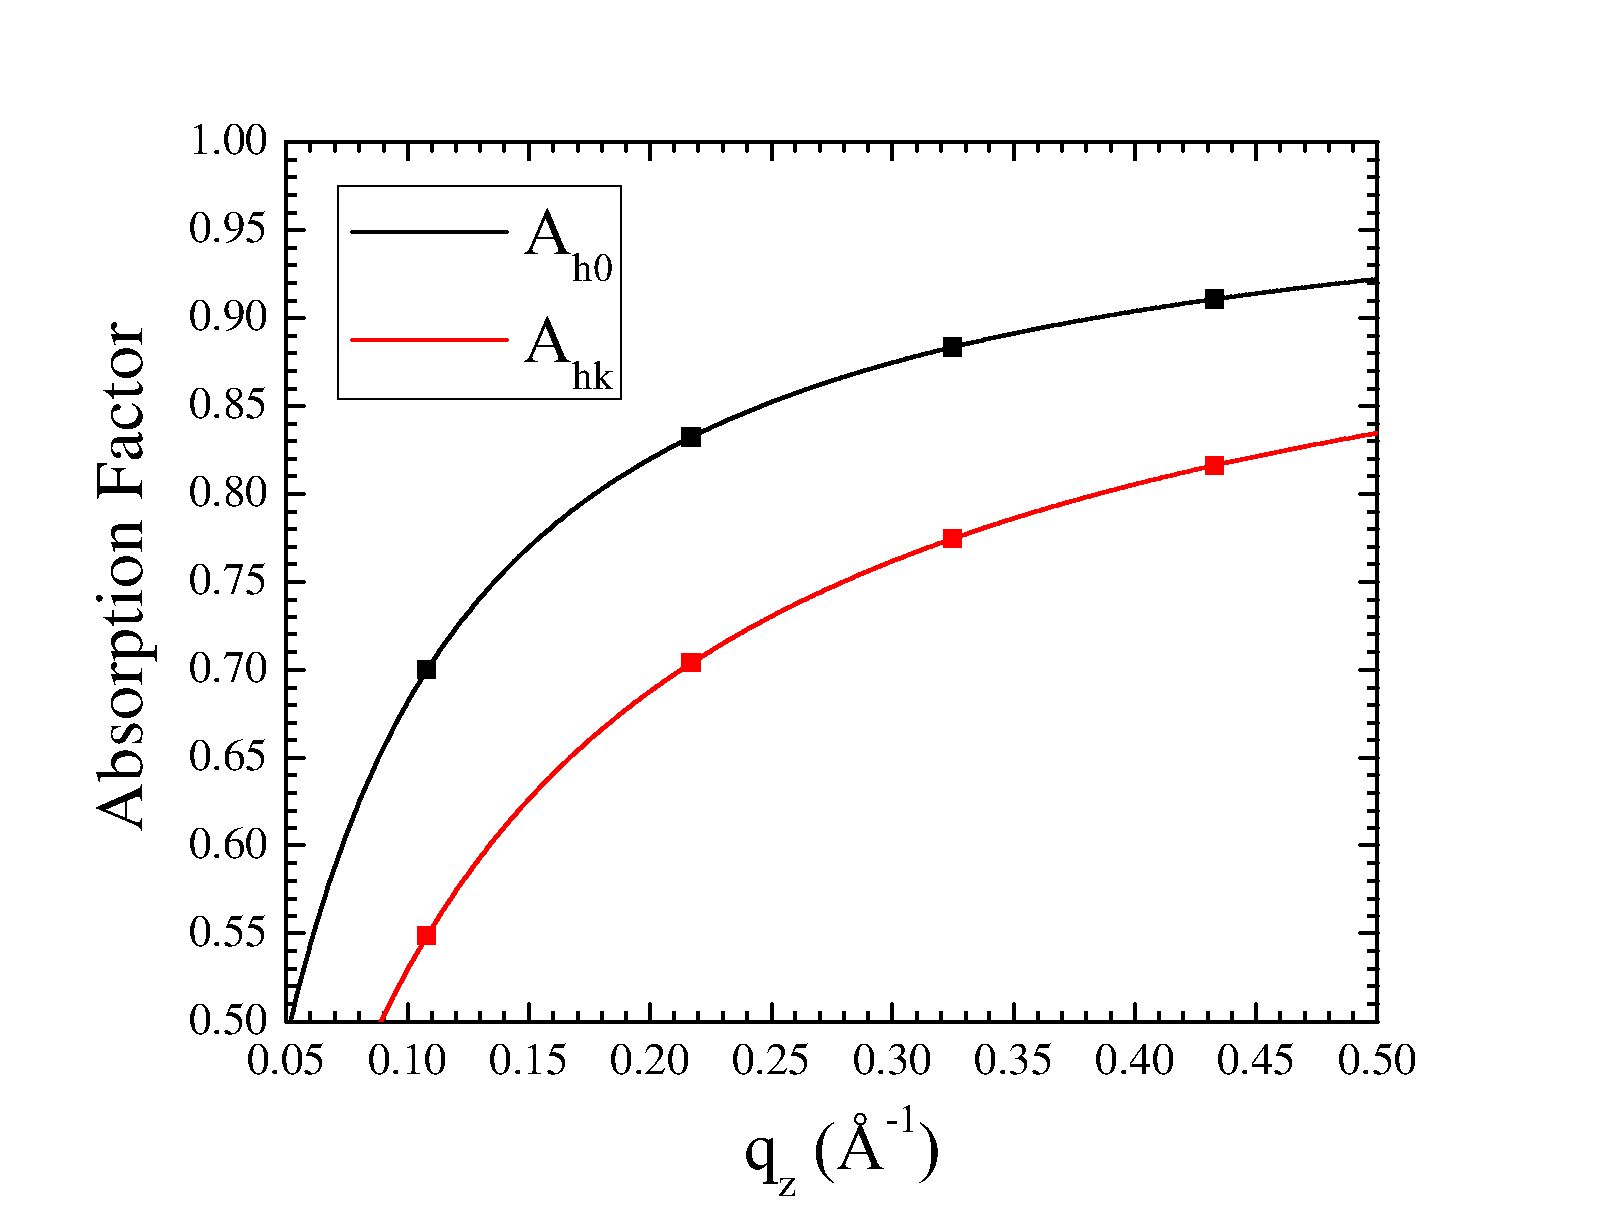
\includegraphics[width=0.8\textwidth]{figures/ripple/analysis/abs_factor}
  \caption{Absorption factors as a function of $q_z \approx 4\pi\theta/\lambda$.
  Values at $q_z=2\pi h/D$ corresponding to $D=57.8$ \AA\ are shown as squares.
  $\mu$ = 2600 $\mu$m, $t$ = 10 $\mu$m, and $\lambda$ = 1.175 \AA.}
  \label{fig:abs_factor}
\end{figure}
%------------------------------------------------------------------------------

For $k\neq 0$ side peaks, an integration over the incident angle $\omega$
is necessary because these peaks are observable at all our experimental incident angles as
described in section \ref{sec:Lorentz_correction}.
The total observed intensity from a rotating sample is simply
\begin{equation}
  I_{\textrm{total}}(\theta) 
  = \int_0^{2\theta}\textrm{d}\omega I_{\textrm{obs}}(\omega,\theta).
  \label{eq:total_obs_I}
\end{equation}
The upper integration limit is equal to $2\theta$ because the substrate
completely blocks the scattered X-rays above this angle as discussed in 
section \ref{sec:Lorentz_correction}.
The total non-attenuated intensity is equal to $2\theta t I_0$. We, then, 
define the absorption factor $A(\theta)$ to be the ratio of the total 
observed intensity to the total non-attenuated intensity,
\begin{align}
  A(\theta) \equiv \frac{I_\textrm{total}(\theta)}{2\theta tI_0}. 
  \label{eq:abs_factor_def}
\end{align}
Using Eq.~(\ref{eq:ang_abs_factor}) and (\ref{eq:total_obs_I})
in (\ref{eq:abs_factor_def}), we arrive
at the final absorption factor
\begin{equation}
  A(\theta) = \frac{1}{2\theta}\int_0^{2\theta}d\omega A(\omega,\theta)
  = \frac{\mu}{2\theta t} \int_0^{2\theta}d\omega 
  \frac{1-\exp\left(-\frac{t}{\mu}g(\omega,\theta)\right)}{g(\omega,\theta)}.
  \label{eq:abs_factor}
\end{equation}
$A_{hk} = A(\theta)$ is plotted in Fig.~\ref{fig:abs_factor}.
The absorption correction $A_c(\theta)$ is the inverse of Eq.~(\ref{eq:abs_factor}). 


%%%%%%%%%%%%%%%%%%%%%%%%%%%%%%%%%%%%%%%%%%%%%%%%%%%%%%%%%%%%%%%%%%%%%%%%%%%%%%%
\subsection{Correction due to mosaic spread}\label{sec:mosaic_spread_correction}
(Under construction)
Integrated intensity needs to be corrected for mosaic spread. 
During an X-ray exposure, the sample
was continuously rotated. Due to this rotation, each pixel integrates 
intensity over the incident angle $\omega$.
As described in
appendix~\ref{app:mosaic_exp}, a rocking scan probes a mosaic spread distribution
as a function of $\omega$, so integrated intensity observed on a detector 
is proportional to an integrated mosaic spread distribution.
Because the range of the distribution probed is limited by 
$\omega=2\theta_B$. this range is larger for higher orders. The observed 
integrated intensity is then larger for higher orders even if the intrinsic
relative intensity of different orders is the same. This effect is 
illustrated in Fig.~\ref{fig:mosaic_contour}.

\begin{figure}[htbp]
  \centering
  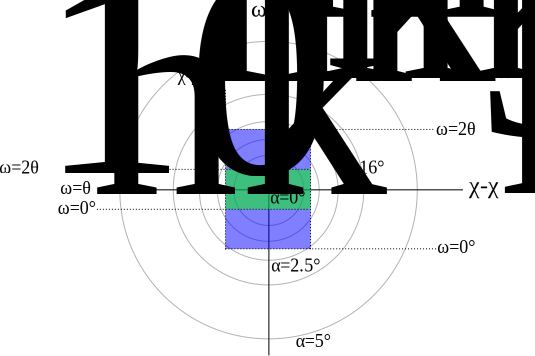
\includegraphics[width=0.9\textwidth]{figures/ripple/analysis/mosaic_contour}
  \caption{Contours of a mosaic spread distribution projected on the $xy$-plane.
  The distribution function takes a form of Lorentzian centered at $\alpha=0$.
  Domains with $\alpha=0$ are probed at $\omega=\theta_B$ and $\chi=0$.
  Integrated intensity of $(1,0)$ reflection is proportional to the green
  shaded area while that of $(3,0)$ reflection is proportional to the
  blue shaded area, which is three times larger. The rocking scan axis
  is centered at $\theta_B$.}
  \label{fig:mosaic_contour} 
\end{figure}

We limit 
$\chi$ to go from -1.4\textdegree\ to 1.4\textdegree. This simplifies a calculation
because we can ignore the curvature of the sphere on which the mosaic spread
distribution $P(\alpha)$ is defined as described in Appendix~\ref{app:mosaic_calc}.
The effect of cutoff on $\chi$ is not very important
because most of observed intensity was included in integration boxes.
In contrast, cutoff on $\omega$ due to substrate blocking the scattering
is important, especially for lower $h$ orders.
 
We take the distribution to be Lorentzian, which has been experimentally
observed.
\begin{equation}
  P(\alpha) = \frac{N}{\alpha^2+\alpha_M},
\end{equation}
where $N$ is a normalization constant and $\alpha_M$ is the HWHM of the 
distribution. $N$ satisfies
\begin{equation}
  N \approx \frac{1}{2\pi}\left(\int_0^{\frac{\pi}{2}}\mathop{d\alpha}
  \frac{\alpha}{\alpha^2+\alpha_M^2}\right)^{-1},
  \label{eq:mosaic_N}
\end{equation}
where a small angle approximation is assumed for $\alpha$.
We then imagine a two dimensional contour map on a $\omega\chi$ plane.
Observed intensity for a Bragg peak with a Bragg angle of $\theta_B$ is
given by
\begin{equation}
  I^\textrm{obs}_{h0} = \int_{-\theta_B}^{\theta_B}\mathop{d\omega} 
  \int_{-\chi_0}^{\chi_0}\mathop{d\chi} P(\alpha)
  = \int_{-\theta_B}^{\theta_B}\mathop{d\omega}
  \int_{-\chi_0}^{\chi_0}\mathop{d\chi}
  \frac{N}{(\omega-\theta_B)^2+\chi^2+\alpha_M^2}
  \label{eq:mosaic_I}
\end{equation}
After $\chi$ integration, Eq.~(\ref{eq:mosaic_I}) is
\begin{equation}
  I^\textrm{obs}_{h0} = 4N\int_0^{\theta_B}\frac{d\omega}{\sqrt{\omega^2+\alpha_M^2}}
  \arctan\pars{\frac{\chi_0}{\sqrt{\omega^2+\alpha_M^2}}}.
  \label{eq:mosaic_I2}
\end{equation}
Eq.~(\ref{eq:mosaic_I2}) is plotted in Fig.~\ref{fig:mosaic_correction}.

\begin{figure}
  \centering
  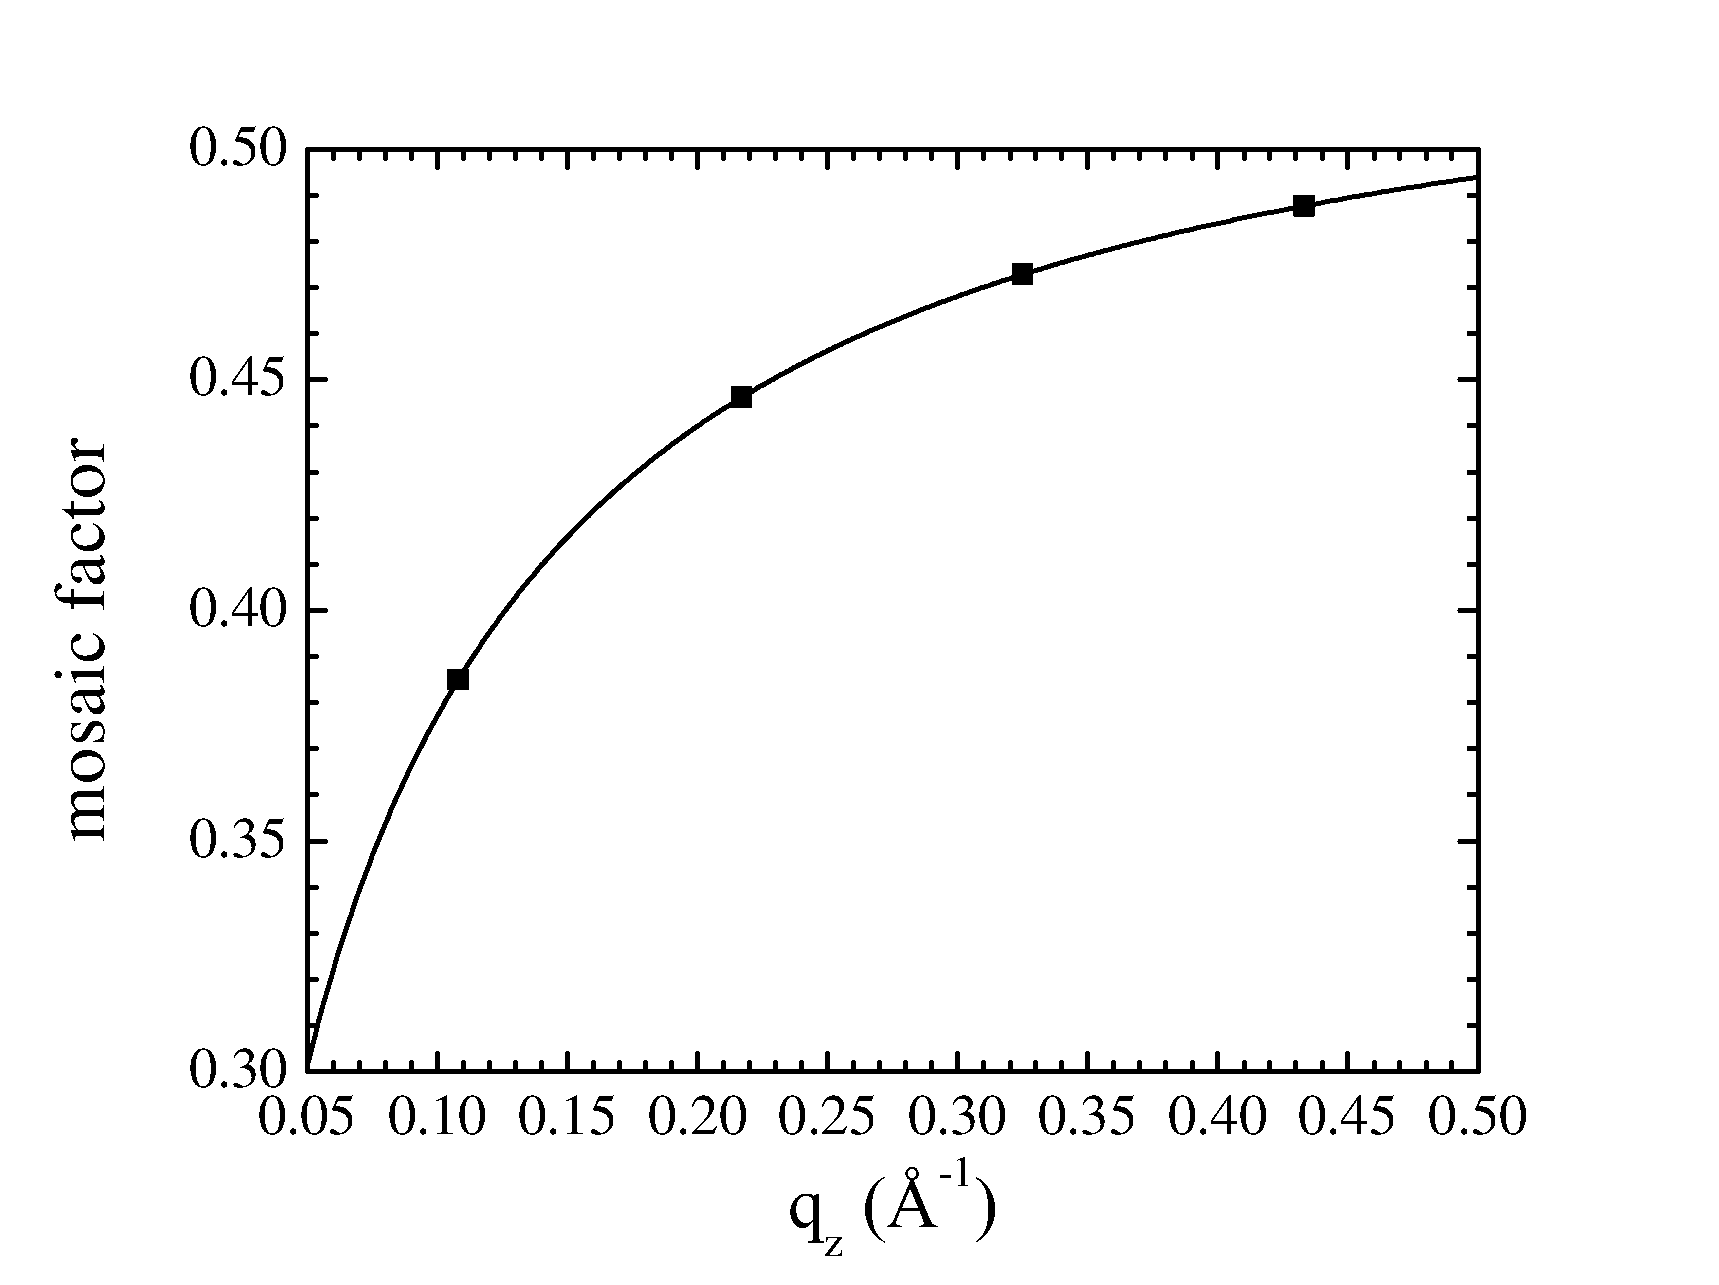
\includegraphics[width=0.7\textwidth]{figures/ripple/analysis/mosaic_correction}
  \caption[Mosaic factor given by Eq.~(\ref{eq:mosaic_I2}) as a function of 
  $q_z\approx 4\pi\theta/\lambda$]{Mosaic factor given by Eq.~(\ref{eq:mosaic_I2}) as a function of 
  $q_z\approx 4\pi\theta/\lambda$. Values at $q_z=2\pi h/D$ corresponding to $D=57.8$ \AA
  are shown as squares. $\alpha_M=0.05$\textdegree and $\chi_0$=1.4\textdegree.}
  \label{fig:mosaic_correction}
\end{figure}

%As Fig.~\ref{fig:rocking_scan_data} shows, observed intensity of $(h,k\neq 0)$ reflections are independent
%of the incident angle $\omega$. Therefore, they do not need to be corrected 
%for mosaic spread. Essentially, this mosaic spread correction is due to
%the substrate blocking incoming and outgoing X-rays outside a range of 
%incident angles. Because this effect is already taken
%into account for $(h,k\neq 0)$ side peaks in the Lorentz correction
%as described in Sec.~\ref{sec:Lorentz_correction}, 
%the mosaic spread correction is not necessary for the side peaks.  
%
%\begin{figure}
%  \centering
%  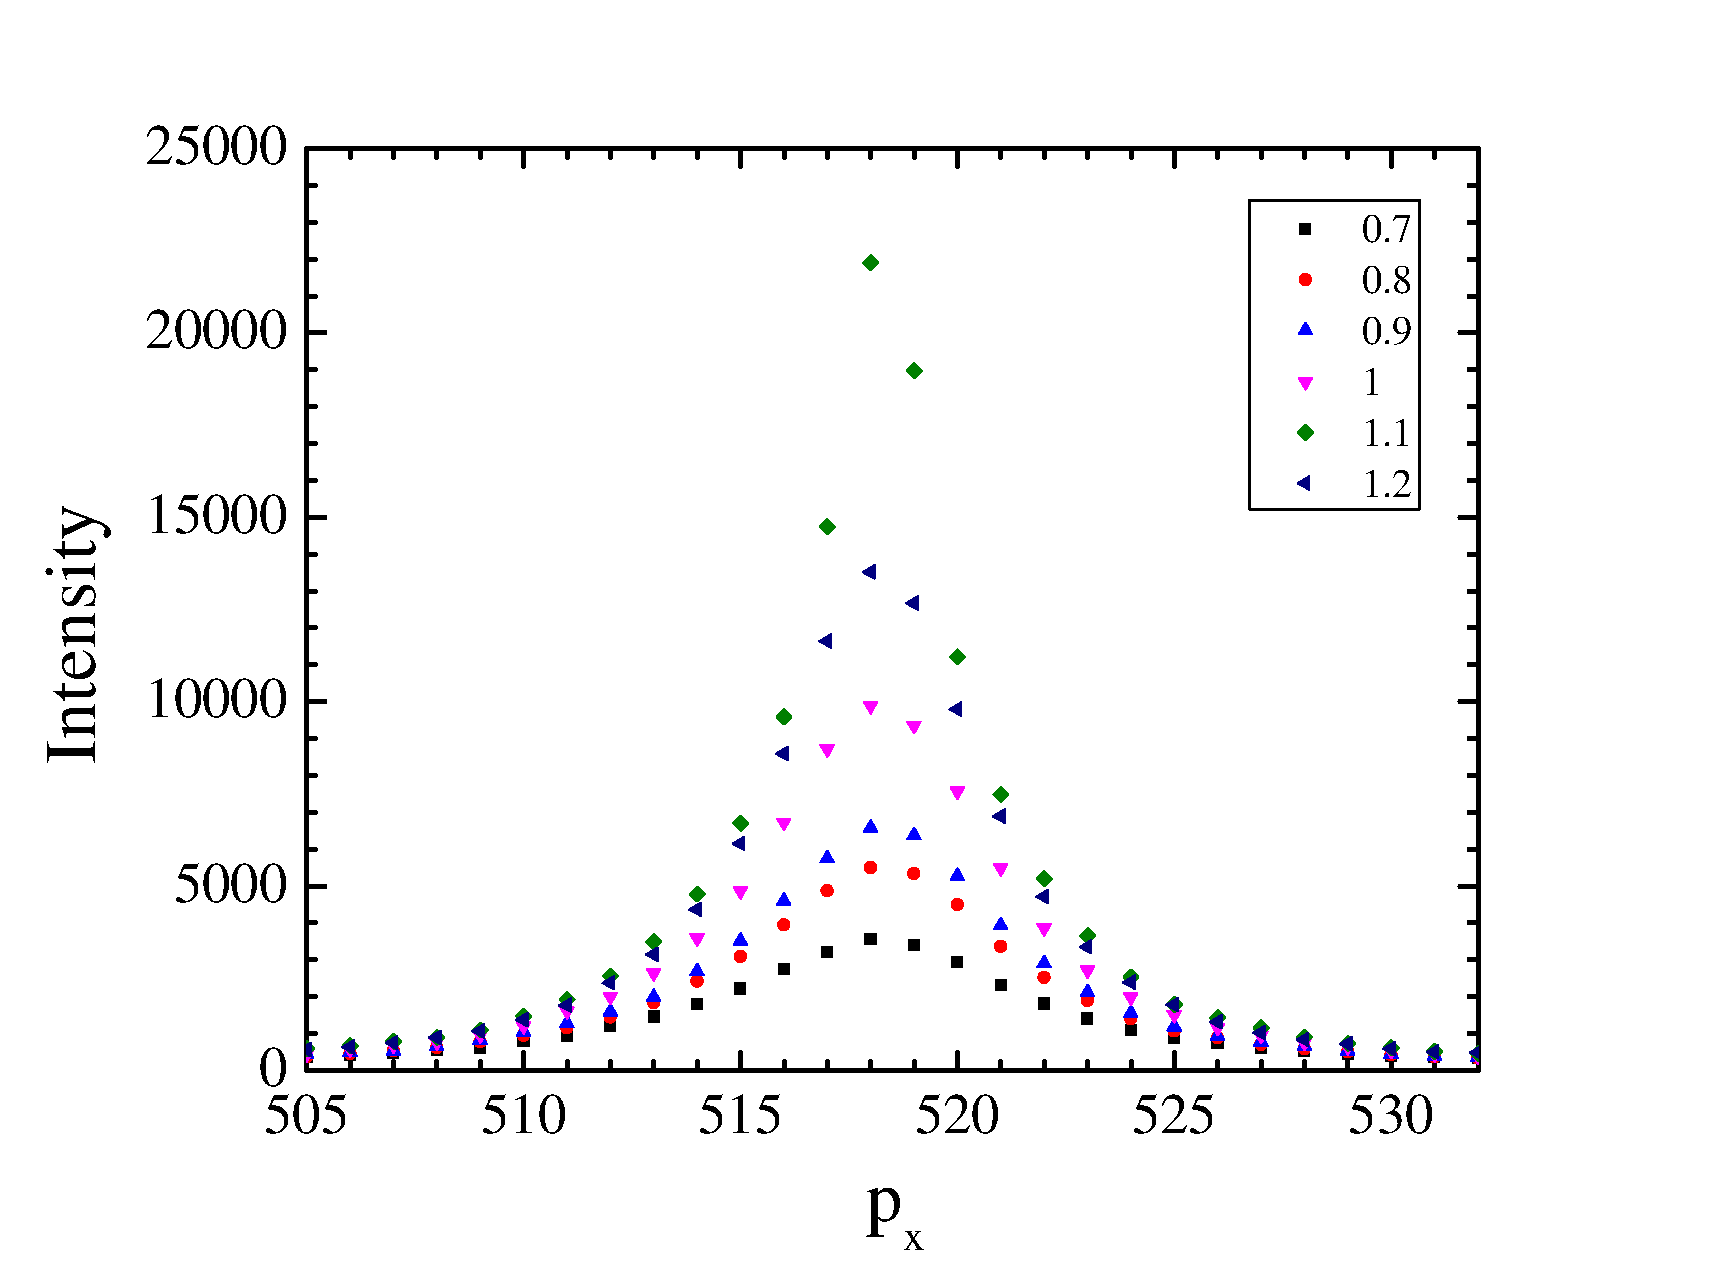
\includegraphics[width=0.45\textwidth]{figures/ripple/analysis/20peaks}
  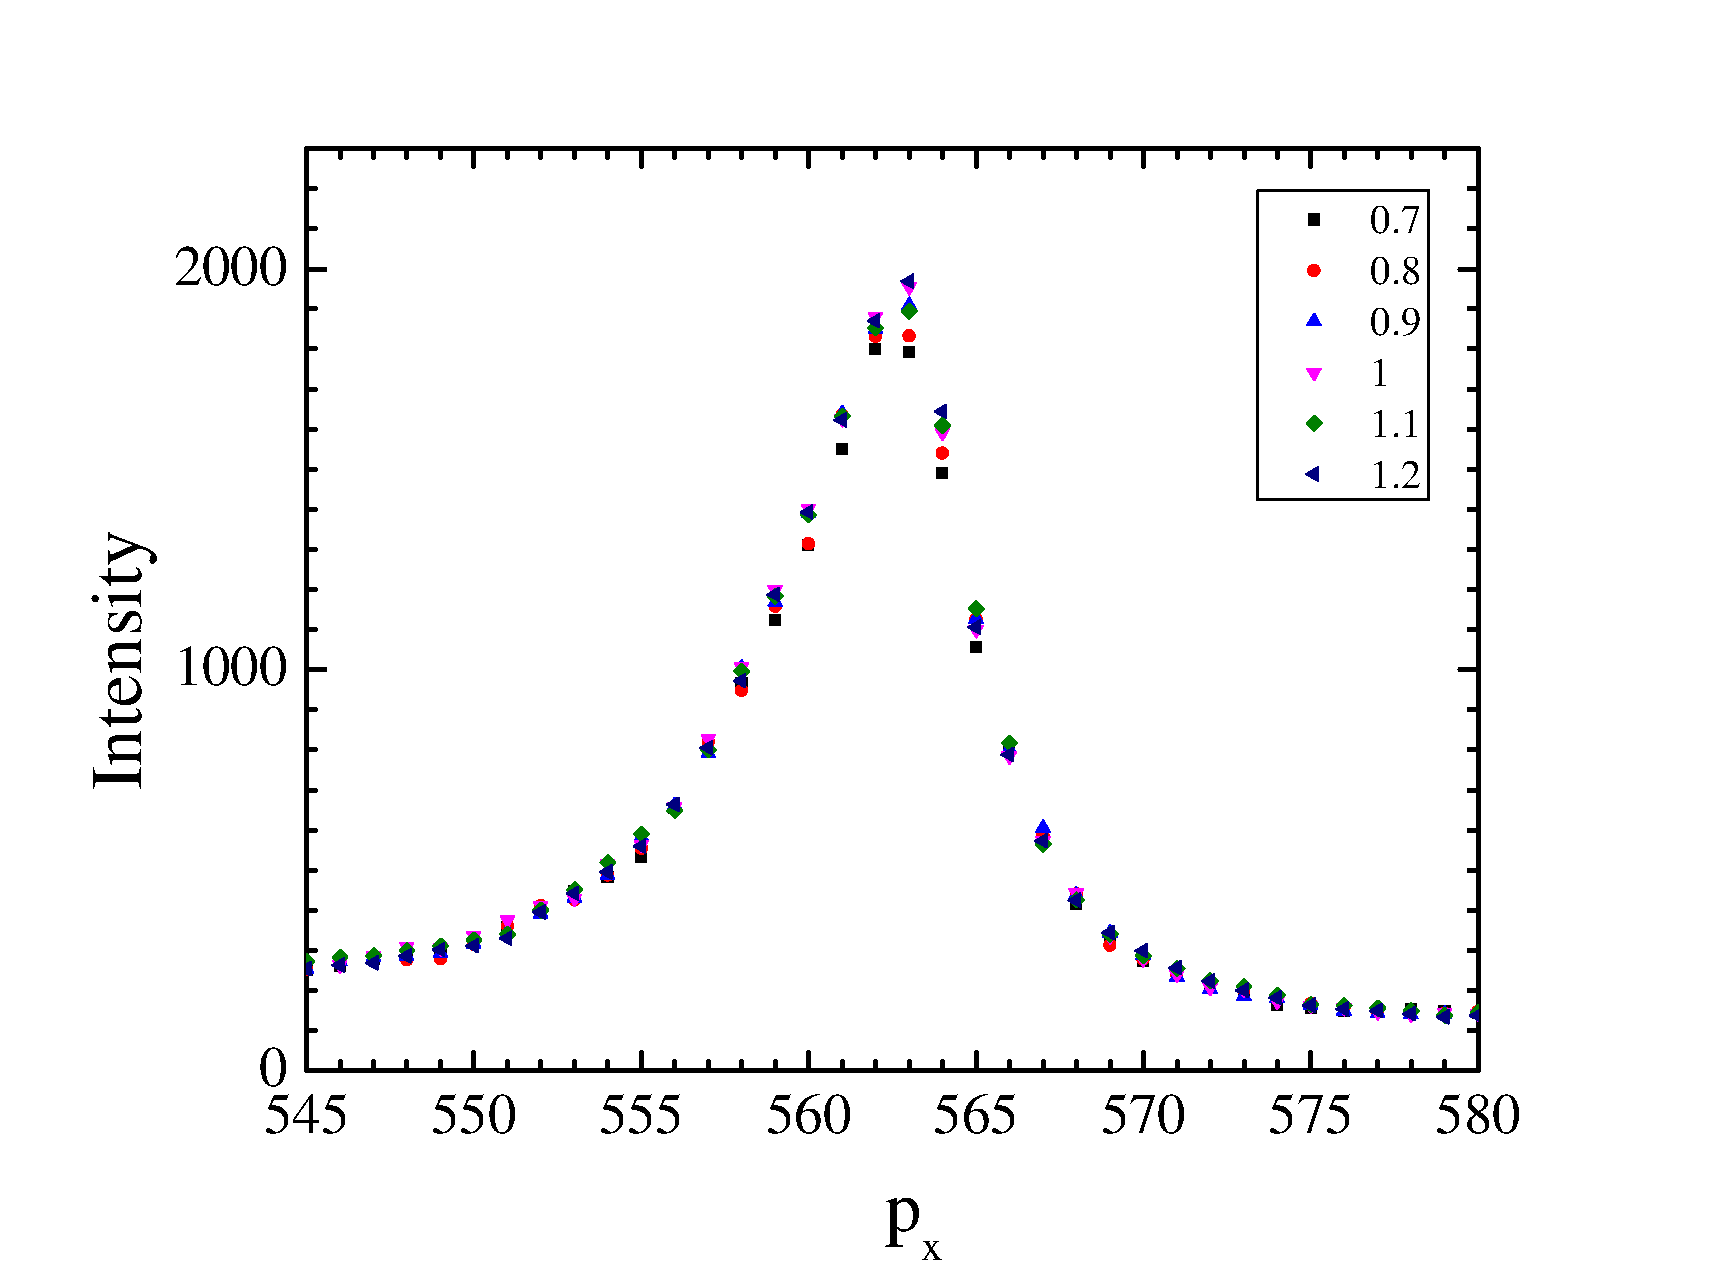
\includegraphics[width=0.45\textwidth]{figures/ripple/analysis/21peaks}
%  \caption[title goes here]{caption goes here}
%  \label{fig:rocking_scan_data}
%\end{figure} 

%%%%%%%%%%%%%%%%%%%%%%%%%%%%%%%%%%%%%%%%%%%%%%%%%%%%%%%%%%%%%%%%%%%%%%%%%%%%%%%
\section{LAXS: model}
\subsection{Contour Part of the Form Factor}\label{sec:contour}
As in Ref.\cite{ref:Sun96}, we take the ripple profile to have a sawtooth profile. Its
amplitude is $A$ and the projection of the major arm on the 
ripple direction is $\xM$ as shown in Fig.~\ref{fig:unit_cell}. 
Then, we write the ripple profile as
\begin{equation}
  u(x) = \left\{
    \begin{array}{ccc}
    -\frac{A}{\lambda_r-x_0}\left(x+\frac{\lambda_r}{2}\right) 
      & \text{for} 
      & -\frac{\lambda_r}{2} \leq x < -\frac{x_0}{2}, \\
    \frac{A}{x_0}x 
      & \text{for} 
      & -\frac{x_0}{2} \leq x \leq \frac{x_0}{2}, \\
    -\frac{A}{\lambda_r-x_0} \left(x-\frac{\lambda_r}{2}\right)
      & \text{for} 
      & \frac{x_0}{2} < x \leq \frac{\lambda_r}{2}.
    \end{array} \right.
  \label{eq:sawtooth}
\end{equation}
The ripple profile has inversion symmetry, so that the resulting
form factor is real. $A$ and $\xM$ are fitting parameters that depend 
on the integrated intensity of each peak while $D$, $\lambda_r$, and $\gamma$
are determined from measuring the positions of the Bragg peaks.

In order to allow the electron density along the ripple direction to 
modulate, we include two additional parameters, one to allow for the electron
density across the minor side to be different by a ratio $f_1$ from the 
electron density across the major side and a second parameter $f_2$, which
is multiplied by $\delta$ functions $\delta(x \pm \xM/2)$ to allow for 
a different electron density near the kink between the major and the minor
sides. 

The contour part of the form factor $F_C$ calculated from Eq.~(\ref{eq:sawtooth})
is plotted in Fig.~(\ref{fig:FT}).

\begin{figure}
  \centering
  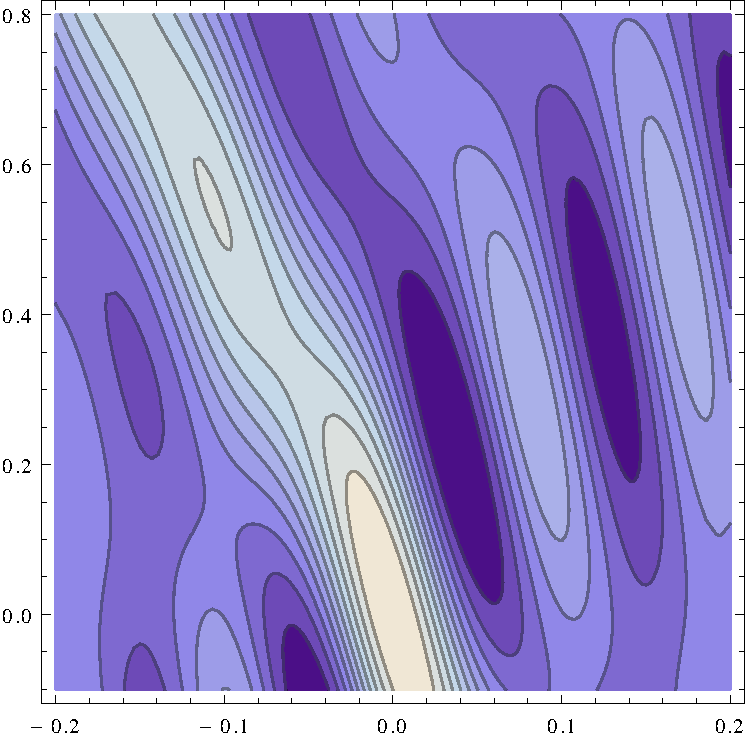
\includegraphics[width=0.5\textwidth]{figures/ripple/model/F_contour}
  \caption[title goes here]{Not sure if this plot is useful.}
  \label{fig:FT}
\end{figure}

%%%%%%%%%%%%%%%%%%%%%%%%%%%%%%%%%%%%%%%%%%%%%%%%%%%%%%%%%%%%%%%%%%%%%%%%%%%%%%%
\subsection{Transbilayer Part of the Form Factor}\label{sec:transbilayer}
\subsubsection{Delta function model}
Delta function model is described here.

\subsubsection{1G and 2G hybrid model}
In the hybrid model, the terminal methyl region of the bilayer is represented
as a Gaussian function \cite{ref:Wiener89}. The headgroups are represented by one 
and two Gaussian
functions in 1G and 2G hybrid model, respectively. The methylene and water 
regions are each treated as a constant. The gap between the two constants is 
represented by a sine function. Then, for half of the bilayer, 
$0 \leq z \leq D/2$, the electron density has the form, 
\begin{equation}
  \rho(z) = \rhog(z) + \rhos(z) + \rhob(z),
\end{equation}
where the Gaussian part is given by 
\begin{equation}
  \rhog(z) = \sum_{i=1}^{1\text{ or }2} \rhoh{i}
             e^{-(z-\zh{i})^2/(2\sigmah{i}^2)} + \rhom e^{-z^2/(2\sigmam^2)},
\end{equation}
the strip part is given by
\begin{equation}
  \rhos(z) = \left\{
    \begin{array}{ccc}
      \rhochtwo & \text{for } & 0 \leq z < \zchtwo, \\
      \rhow   & \text{for } & \zw \leq z \leq D/2,
    \end{array}
  \right.
\end{equation}
and the bridging part is given by
\begin{equation}
  \rhob(z) = \frac{\rhow-\rhochtwo}{2} \cos \bracks{
    \frac{-\pi}{\deltazh}(z-\zw)} + \frac{\rhow+\rhochtwo}{2} \\
  \text{\quad for \quad} \zchtwo < z < \zw.
\end{equation}
with $\deltazh=\zw-\zchtwo$. Here, we assume $\zh{2}>\zh{1}$. 
Table \ref{tb:zchtwozw} shows some of the definitions.

%------------------------------------------------------------
\begin{table}[htb]
  \centering
  \begin{tabular}{c c c}
     & 1G & 2G \\
    $\zchtwo$ & $\zh{1}-\sigmah{1}$ & $\zh{1}-\sigmah{1}$ \\
    $\zw$ & $\zh{1}+\sigmah{1}$ & $\zh{2}+\sigmah{2}$   
  \end{tabular}
  \caption{Definitions of $\zchtwo$ and $\zw$}
  \label{tb:zchtwozw}
\end{table}
%------------------------------------------------------------

The transbilayer profile along $x=-z\tan\psi$ can be obtained by rotating
the coordinates $x$ and $z$ by $\psi$ in the clockwise direction and
reexpressing $\rho(z)$ in terms of the rotated coordinates. This leads
to replacing $x$ with $x'=x\cos\psi+z\sin\psi$ and
$z$ with $z'=-x\sin\psi+z\cos\psi$. Then, the rotated transbilayer profile is
\begin{equation}
  \rho(x,z) = \delta(x+z\tan\psi)\bracks{\rhog(z') + \rhos(z') + \rhob(z')}.
  \label{eq:rotated_profile}
\end{equation}

Taking the two dimensional Fourier transform of Eq.~(\ref{eq:rotated_profile})
leads to the transbilayer part of the form factor,
\begin{align}
  F_\mathrm{T} 
  &= \int_{-\frac{D}{2}}^{\frac{D}{2}} \int_{-\frac{\lambda_r}{2}}^{\frac{\lambda_r}{2}} 
     \bracks{\rho(x,z)-\rhow} e^{i(q_xx+q_zz)} dxdz \\
  &= F_\mathrm{G} + F_\mathrm{S} + F_\mathrm{B}.
\end{align}
The form factor is calculated in the minus fluid convention, 
where the bilayer electron density
is measured with respect to the electron density of the surrounding solvent.
The expression for $F_\mathrm{T}$ is rather messy, so 
the derivation and full expression are in the appendix. Here, 
we note that
the fitting parameters in this model are $\zh{i}$, $\sigmah{i}$, and 
$\Rhm{i}$ for each of the two headgroup Gaussian functions, $\sigmam$ for
the terminal methyl Gaussian, $\Delta R$ for the methylene region, $\psi$ for
the lipid tilt, and an overall scaling factor. The contour part of the 
form factor has four more parameters ($A$, $\xM$, $f_1$, and $f_2$).
In total, the modified 2G hybrid model implements 14 structural parameters.

%%%%%%%%%%%%%%%%%%%%%%%%%%%%%%%%%%%%%%%%%%%%%%%%%%%%%%%%%%%%%%%%%%%%%%%%%%%%%%%
\section{LAXS: results}
\subsection{Data and Electron Density Profile}\label{sec:LAXS}
Table~\ref{tb:obs_intensity1} and \ref{tb:obs_intensity2} summarize observed intensity from data shown
in Fig.~\ref{fig:ripple_laxs_images}. $q_z$ values for observed peaks were
corrected for index of refraction (Appendix~\ref{app:refraction}).
We measured scattering on oriented samples in almost identical conditions as the
best unoriented sample of Wack and Webb. As discussed earlier,
these two types of samples have different Lorentz corrections, so 
this allowed us to check our data obtained on 
oriented samples against an unoriented sample. 
As Table~\ref{tb:obs_intensity1} shows, agreement between our oriented data
and the uroriented data was good, but integrated intensity from our oriented
sample was in many cases larger than that from an unoriented sample.
We attribute this discrepancy to the way intensity was extracted. 
In an X-ray data from an oriented sample, each peak
was nicely separated, so integrating a peak intensity was rather trivial.
In contrast, some reflections in unoriented data were overlapping with
each other (three pairs of overlapping peaks are highlighted in Table~\ref{tb:obs_intensity1}), 
making separation of intensity difficult. If the $(1,0)$ peak in the unoriented 
data were overestimated, that would account for the observed discrepancy.
Indeed, the microdensitometer trace in \cite{ref:Wack89} suggests that 
the $(1,0)$ and $(1,1)$ reflections should have similar intensity.

\begin{table}[htbp]
  \centering
  \begin{tabular}{rrrrrr}
    \hline
    \multicolumn{1}{c}{$h$} & \multicolumn{1}{c}{$k$} & \multicolumn{1}{c}{$q_z$} & \multicolumn{1}{c}{$q_r$} & \multicolumn{1}{c}{$\Io{hk}$} & \multicolumn{1}{c}{box size} \\
     & & \multicolumn{1}{c}{(\AA$^{-1}$)} & \multicolumn{1}{c}{(\AA$^{-1}$)} & & \multicolumn{1}{c}{(pixels)} \\ 
    \hline
    1 & -1 & 0.102 &-0.043 & 726 & 10 $\times$ 7 \\
    1 &  0 & 0.109 &0.000 & 180818 & 10 $\times$ 7 \\
    1 &  1 & 0.114 &0.043 &    241 & 10 $\times$ 7 \\
    1 &  3 & 0.128 &0.130 &	   4.8 & 10 $\times$ 7 \\
    2 & -2 & 0.206 &-0.087 &	  51.4 & 10 $\times$ 7 \\
    2 & -1 & 0.212 &0.044&	  1818 & 10 $\times$ 7 \\
    2 &  0 & 0.218 &0.000&10200 & 10 $\times$ 7 \\
    2&1&0.224&0.043&558 & 10 $\times$ 7 \\
    2&2&0.231&0.086&116& 10 $\times$ 7 \\
    2 &  3 & 0.23  &  0.129 &	    27 & 10 $\times$ 7 \\
    2 &  4 & 0.243 &  0.173 &    7.6 & 10 $\times$ 7 \\
    2 &  5 & 0.250 &  0.214 &    2.9 & 10 $\times$ 7 \\
    3 &	-2 & 0.314 & -0.087 & 305 & 15 $\times$ 7 \\
    3 & -1 & 0.321 & -0.043	&   1205 & 15 $\times$ 7 \\
    3 &  0 & 0.326 &  0.000 & 1566 & 15 $\times$ 7 \\
    3 &  1 & 0.333 &  0.043 &   31.7 & 15 $\times$ 7 \\
    3 &  2 & 0.339 &  0.086 &   32.4 & 15 $\times$ 7 \\
    3 &  3 & 0.345 &  0.129 &	  38.2 & 15 $\times$ 7 \\
    3 &  4 & 0.352 &  0.172 &	  26.1 & 15 $\times$ 7 \\
    3 &  5 & 0.358 &  0.215 &	   8.6 & 15 $\times$ 7 \\
    \hline
  \end{tabular}
  \begin{tabular}{rrrrr}
    \hline
    \multicolumn{1}{c}{$h$} & \multicolumn{1}{c}{$k$} & \multicolumn{1}{c}{$q$*}& \multicolumn{1}{c}{oriented} & \multicolumn{1}{c}{unoriented} \\
     & & \multicolumn{1}{c}{(\AA$^{-1}$)} & \multicolumn{1}{c}{$|F_{hk}|$} & \multicolumn{1}{c}{$|F_{hk}|$*} \\
    \hline
    1 & -1 & {\color{red}0.111} &  83.0 & 60.8 \\
    1 &  0 & {\color{red}0.108} & 100.0 & 100.0 \\
    1 &  1 & 0.123 &  44.0 & 26.9 \\
    1 &	 3 & 0.185 &   9.9 & 7.6 \\
    2 &	-2 & 0.224 &  19.4 & 15.1 \\
    2 &	-1 & {\color{blue}0.215} &  80.2 & 71.2 \\
    2 &  0 & {\color{blue}0.217} &  30.8 & 39.7 \\
    2 &	 1 & 0.228 &  42.4 & 33.9 \\
    2 &  2 & 0.246 &  26.8 & 22.7 \\
    2 &	 3 & 0.271 &  15.6 & 14.2 \\
    2 &  4 & 0.301 &   9.5 & 7.8 \\
    2 &  5 & 0.329 &   6.4 & \\
	3 &	-2 & {\color{green}0.325} &  36.2 & 29.3 \\
    3 & -1 & 0.322 &  50.0 & 44.2 \\
    3 &  0 & {\color{green}0.325} &  14.4 & 12.0 \\
    3 &  1 & & 7.9 & \\
    3 &  2 & 0.350 &  11.2 & 10.5 \\
    3 &  3 & 0.370 &  14.8 & 14.9 \\
    3 &  4 & 0.394 &  13.9 & 10.0 \\
    3 &  5 & & 8.8 & \\
    \hline
  \end{tabular}
  \caption{Observed intensity for $h$ = 1 to 3 at $D=57.8$, $\lambda_r=145$, and 
  $\gamma=98.2$\textdegree. *Unoriented data are from Wack and Webb \cite{ref:Wack89}.}
  \label{tb:obs_intensity1}
\end{table}

\begin{table}[htbp]
  \centering
  \begin{tabular}{rrrrrr}
    \hline
    \multicolumn{1}{c}{$h$} & \multicolumn{1}{c}{$k$} & \multicolumn{1}{c}{$q_z$} & \multicolumn{1}{c}{$q_r$} & \multicolumn{1}{c}{$\Io{hk}$} & \multicolumn{1}{c}{box size} \\
     & & \multicolumn{1}{c}{(\AA$^{-1}$)} & \multicolumn{1}{c}{(\AA$^{-1}$)} & & \multicolumn{1}{c}{(pixels)} \\ 
    \hline
    4 &	-3 & 0.417 & -0.131 &    143 & 20 by 8 \\
    4 &	-2 & 0.423 & -0.087 &	   730 & 20 by 8 \\
    4	& -1 & 0.429 & -0.043	&    415 & 20 by 8 \\
    4	&  0 & 0.435 &  0.000 &   1938 & 20 by 8 \\
    4	&  1 &       &        &   51.5 & 20 by 8 \\
    4	&  2 & 0.448 &  0.085 &     39 & 20 by 8 \\
    4	&  3 &       &        &   weak & \\
    4	&  4 & 0.461 &  0.173 &    2.1 & 20 by 8 \\
    4	&  5 & 0.467 &  0.215 &    3.2 & 20 by 8 \\
    4 &	 6 & 0.473 &  0.259 &    1.0 & 20 by 8 \\
    5 & -3 & 0.525 & -0.132 &   84.4 & 25 by 9 \\
    5 & -2 & 0.532 & -0.087	&    146 & 25 by 9 \\
    5 & -1 & 0.538 & -0.042	&   64.6 & 25 by 9 \\
    5	&  0 & 0.544 &  0.000	&    259 & 25 by 9 \\
    5	&  1 & 0.550 &  0.040 &   50.2 & 25 by 9 \\
    6 &	-4 & 0.628 & -0.175	& 10.3 & 30 by 10 \\
    6 &	-3 & 0.635 & -0.131	& 13.8 & 30 by 10 \\
    6 & -2 & 0.641 & -0.085	&  9.7 & 30 by 10 \\
    6 & -1 & 0.647 & -0.043 &  2.0 & 30 by 10 \\
    6 &  0 & 0.653 &  0.000	& 69.0 & 30 by 10 \\
    6 &  1 & 0.659 &  0.043 &  2.5 & 30 by 10 \\
    6 &  2 &       &        & weak \\
    6	&  3 & 0.672 &  0.128 &	    42 & 30 by 10 \\
    6	&  4 & 0.679 &  0.170 &     40 & 30 by 10 \\
    7 & -4 & 0.737 & -0.174 &	    42 & 35 by 10 \\
    7	& -3 & 0.743 & -0.130	&     40 & 35 by 10 \\
    7	& -2 & 0.749 & -0.085	&     15 & 35 by 10 \\
    7	& -1 & 0.755 & -0.042	&     27 & 35 by 10 \\
    7 &  0 & 0.760 &  0.000	&     41 & 35 by 10 \\
    9 & -5 &       &        &	  weak & \\
    9 &	-4 & 0.951 & -0.174	&	    19 & 35 by 10 \\
    9 & -3 &       &        &	  weak & \\
    9 & -2 & 0.963 & -0.085 &   21.0 & 35 by 10 \\
	  9	& -1 &       &        &   weak & \\
	  9 &  0 & 0.974 &  0.000	&   21.0 & 35 by 10 \\
    \hline
  \end{tabular}
  \quad
  \begin{tabular}{rrr}
    \hline
     & & \multicolumn{1}{c}{oriented} \\
    \multicolumn{1}{c}{$h$} & \multicolumn{1}{c}{$k$} & \multicolumn{1}{c}{$|F_{hk}|$} \\
    \hline
    4 & -3 & 25.7 \\
4 & -2 & 46.8 \\ 
4 & -1 & 24.7 \\
4 & 0 & 18.1 \\ 
4 & 1 & 8.5 \\ 
4 & 2 & 10.4 \\ 
4 & 3 \\ 
4 & 4 & 3.4 \\
4 & 5 & 4.6 \\ 
4 & 6 & 2.8 \\ 
5 & -3 & 17.3 \\ 
5 & -2 & 18.4 \\ 
5 & -1 & 8.5 \\ 
5 & 0 & 7.3 \\ 
5 & 1 & 7.2 \\ 
6 & -4 & 6.3 \\ 
6 & -3 & 6.3 \\ 
6 & -2 & 4.2 \\ 
6 & -1 & 0.0 \\ 
6 & 0 & 4.1 \\ 
6 & 1 & 0.0 \\ 
6 & 2 & weak\\
6 & 3 & 10.5 \\
6 & 4 & 11.7 \\ 
7 & -4 & 11.6 \\
7 & -3 & 9.7 \\ 
7 & -2 & 4.8 \\ 
7 & -1 & 4.5 \\ 
7 & 0 & 3.4 \\ 
9 & -5 & \\
9 & -4 & \\
9 & -3 & \\
9 & -2 & \\
9 & -1 & \\
9 & 0 &\\
\hline
\end{tabular}
  \caption{Observed intensity for $h$ = 4 to 9 at $D=57.8$, $\lambda_r=145$, and 
  $\gamma=98.2$\textdegree\ (continued from Table~\ref{tb:obs_intensity1}).}
  \label{tb:obs_intensity2}
\end{table}



Show in a table, fitting 
results. Show an edp. Show the thicknesses of both arms. Comment on
some fine features.

%%%%%%%%%%%%%%%%%%%%%%%%%%%%%%%%%%%%%%%%%%%%%%%%%%%%%%%%%%%%%%%%%%%%%%%%%%%%%%%
\section{NGIWAXS: analysis}
\subsection{Absorption Correction}\label{sec:WAXS_abs_correction}
(Under construction)

%%%%%%%%%%%%%%%%%%%%%%%%%%%%%%%%%%%%%%%%%%%%%%%%%%%%%%%%%%%%%%%%%%%%%%%%%%%%%%%
\section{NGIWAXS: model}
\subsection{Thin rod model}\label{sec:WAXS_thin_rod}


%%%%%%%%%%%%%%%%%%%%%%%%%%%%%%%%%%%%%%%%%%%%%%%%%%%%%%%%%%%%%%%%%%%%%%%%%%%%%%%
\section{NGIWAXS: results}\label{sec:NGIWAXS_results}
Figure~\ref{fig:NGIWAXS} shows near grazing incidence Wide Angle X-ray
scattering (NGIWAXS) from an oriented DMPC film in the ripple phase.
As can be seen, hydrocarbon chain scattering did not vary considerably
between the two $D$-spacings. A weak feature that looks like an 
arc coming from the chain peak was observed. This feature extended
out from $\phi$ = 0\textdegree to at least 70\textdegree. This feature
might simply be mosaic spread scattering due to the peak near the equator.
Because mosaic spread of this sample was very small, 
it may also be possible that the feature is not mosaic spread arc,
but comes from the minor arm, indicating
that tilt modulation may occur in the minor arm. Chains are
packed quite tightly, unlike in the fluid phase. (I did rocking scan,
so show the data, and maybe estimate what scattering would look like 
based on Lorentzian distribution.)

Figure~\ref{fig:NGIWAXS_enlarge} shows an enlarged image of the ripple 
phase WAXS at $D$ = 60.8 \AA. We observed a strong peak off the 
equator and a weak one, the center of which was not determined. 
The maximum intensity of the strong peak was at 
$(q_r, q_z) \approx (1.49 \text{\AA}^{-1}, 0.19 \text{\AA}^{-1})$ as shown
in Fig.~\ref{fig:qrplots}. The weak peak was observed near the equator, but 
separation of this peak from the strong one was most visible at 
$q_z = 0.13 \textrm{\AA}^{-1}$ as Fig.~\ref{fig:qrplots} shows. Separation
of the two peaks was possible because of the high resolution experiment. 
In previous runs with the low resolution setup, the ripple peak
appeared as a single wide peak.

\begin{figure}[htbp]
  \centering
  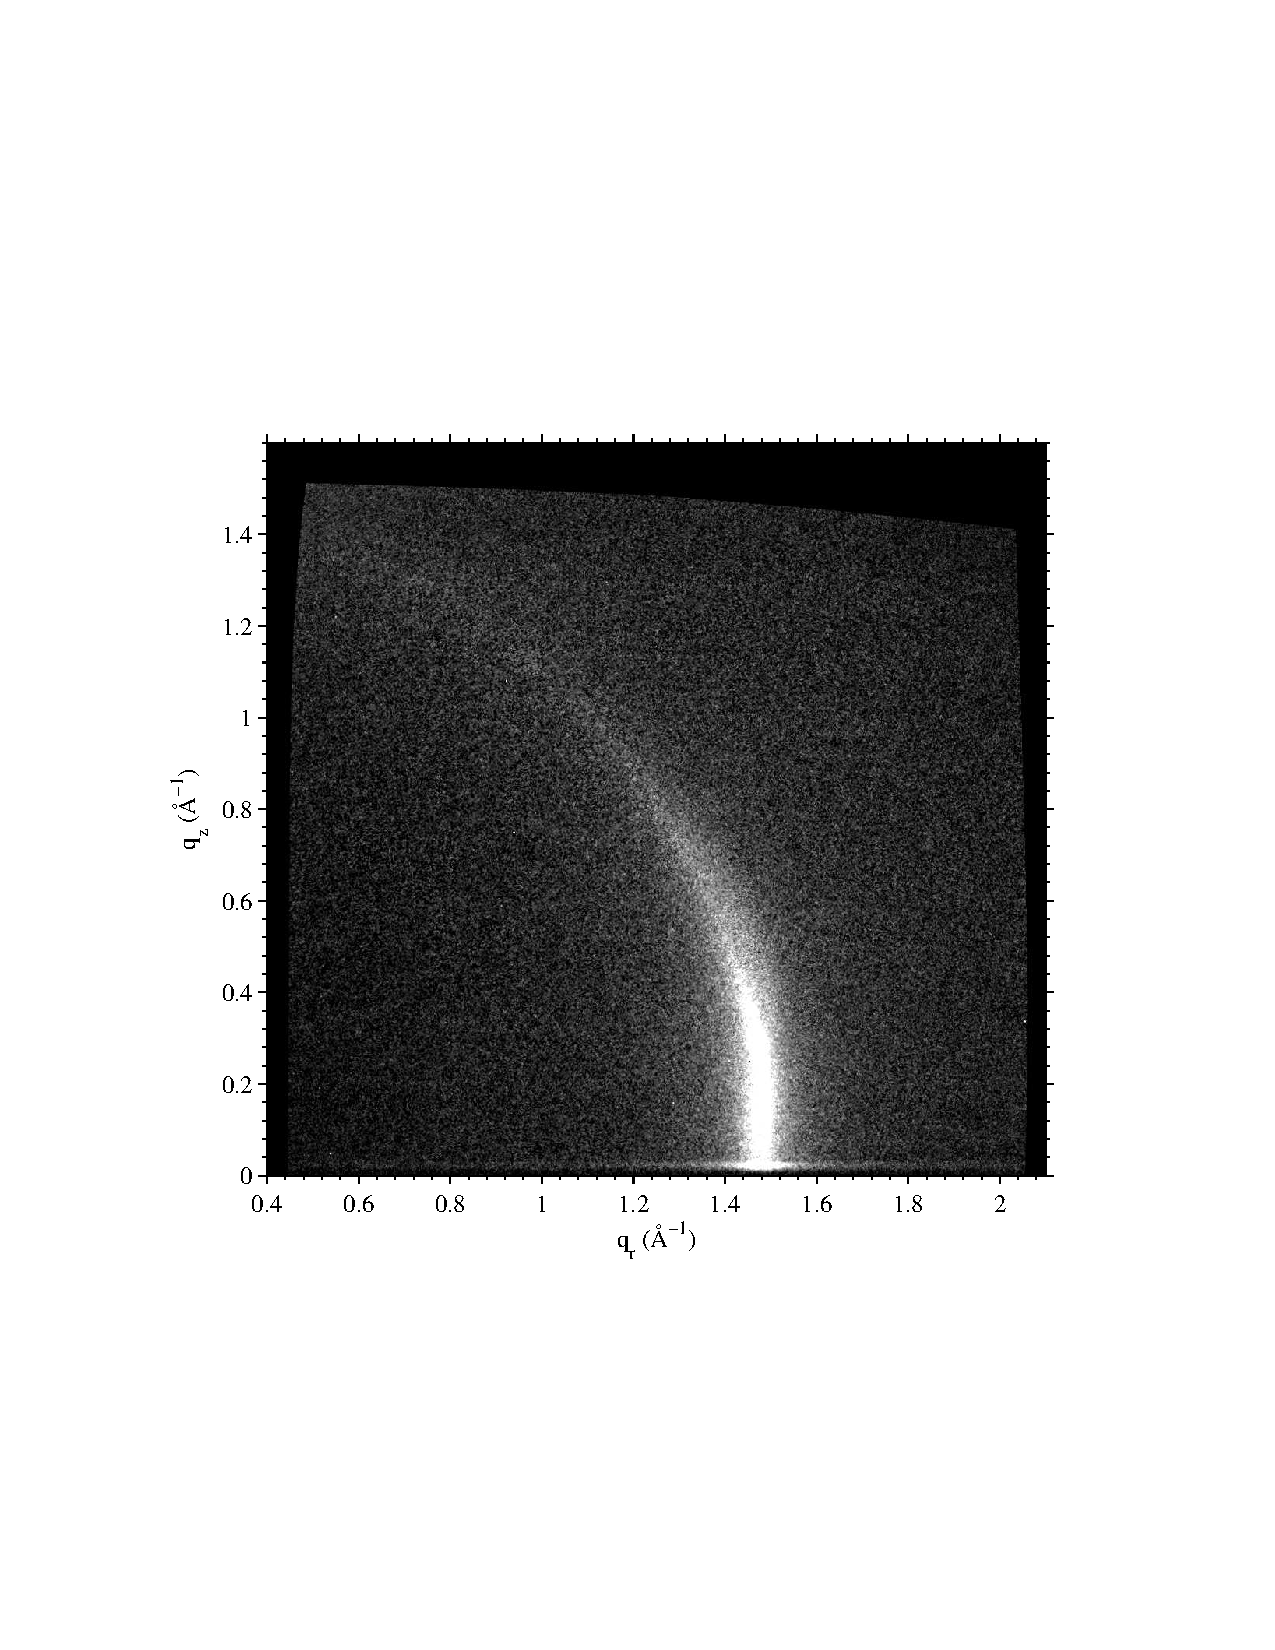
\includegraphics[trim=50 170 50 200,clip,width=0.45\textwidth]{figures/ripple/NGIWAXS/dmpc1_046}
  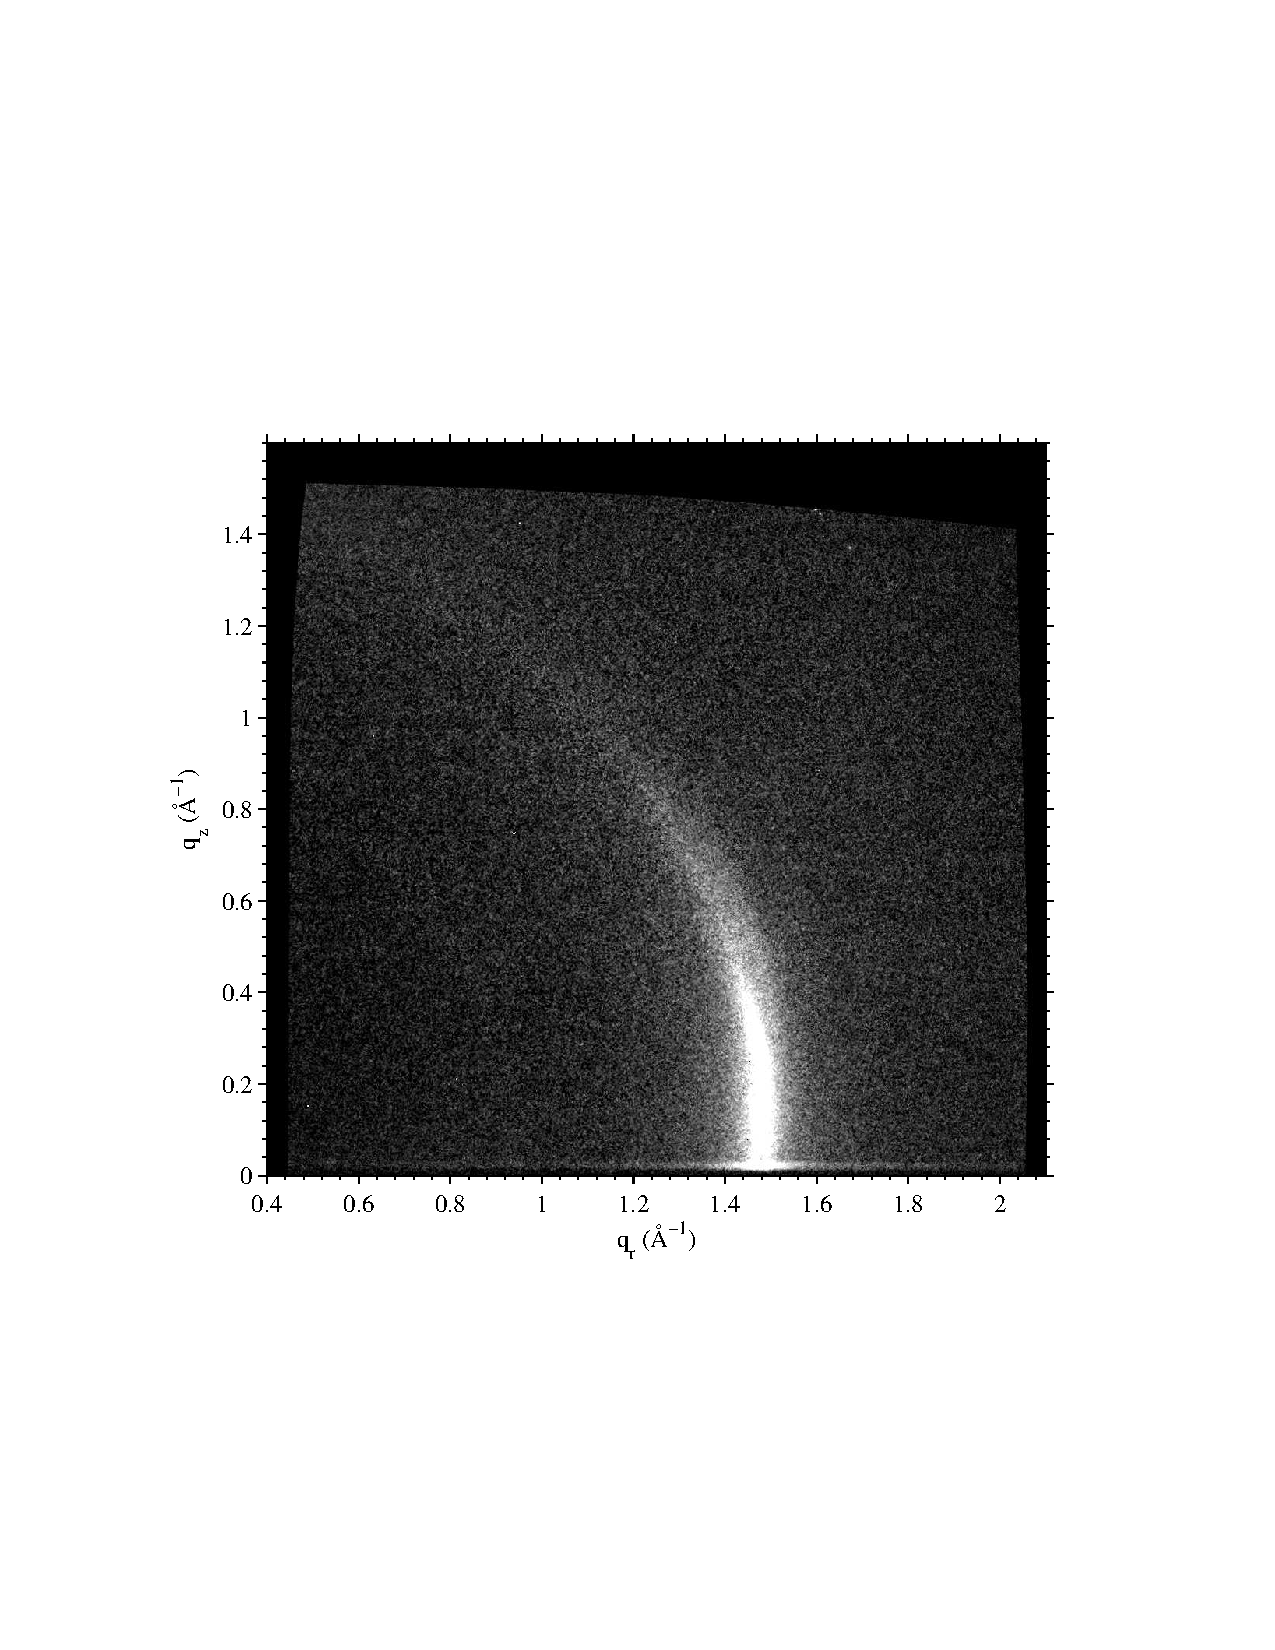
\includegraphics[trim=50 170 50 200,clip,width=0.45\textwidth]{figures/ripple/NGIWAXS/dmpc1_052-060}
  \caption{NGIWAXS of the DMPC ripple phase for $D$ = 59.2 \AA\ (left)
  and 60.8 \AA\ (right). The angle of incidence $\omega$ was 0.2\textdegree.
  The black regions around the edge of each image are the $q$-space that 
  was not probed. The distorted, non rectangular shape of the probed $q$-space
  signifies non-linear relation between the CCD space and sample $q$-space.}
  \label{fig:NGIWAXS}
\end{figure}

\begin{figure}[htbp]
  \centering
  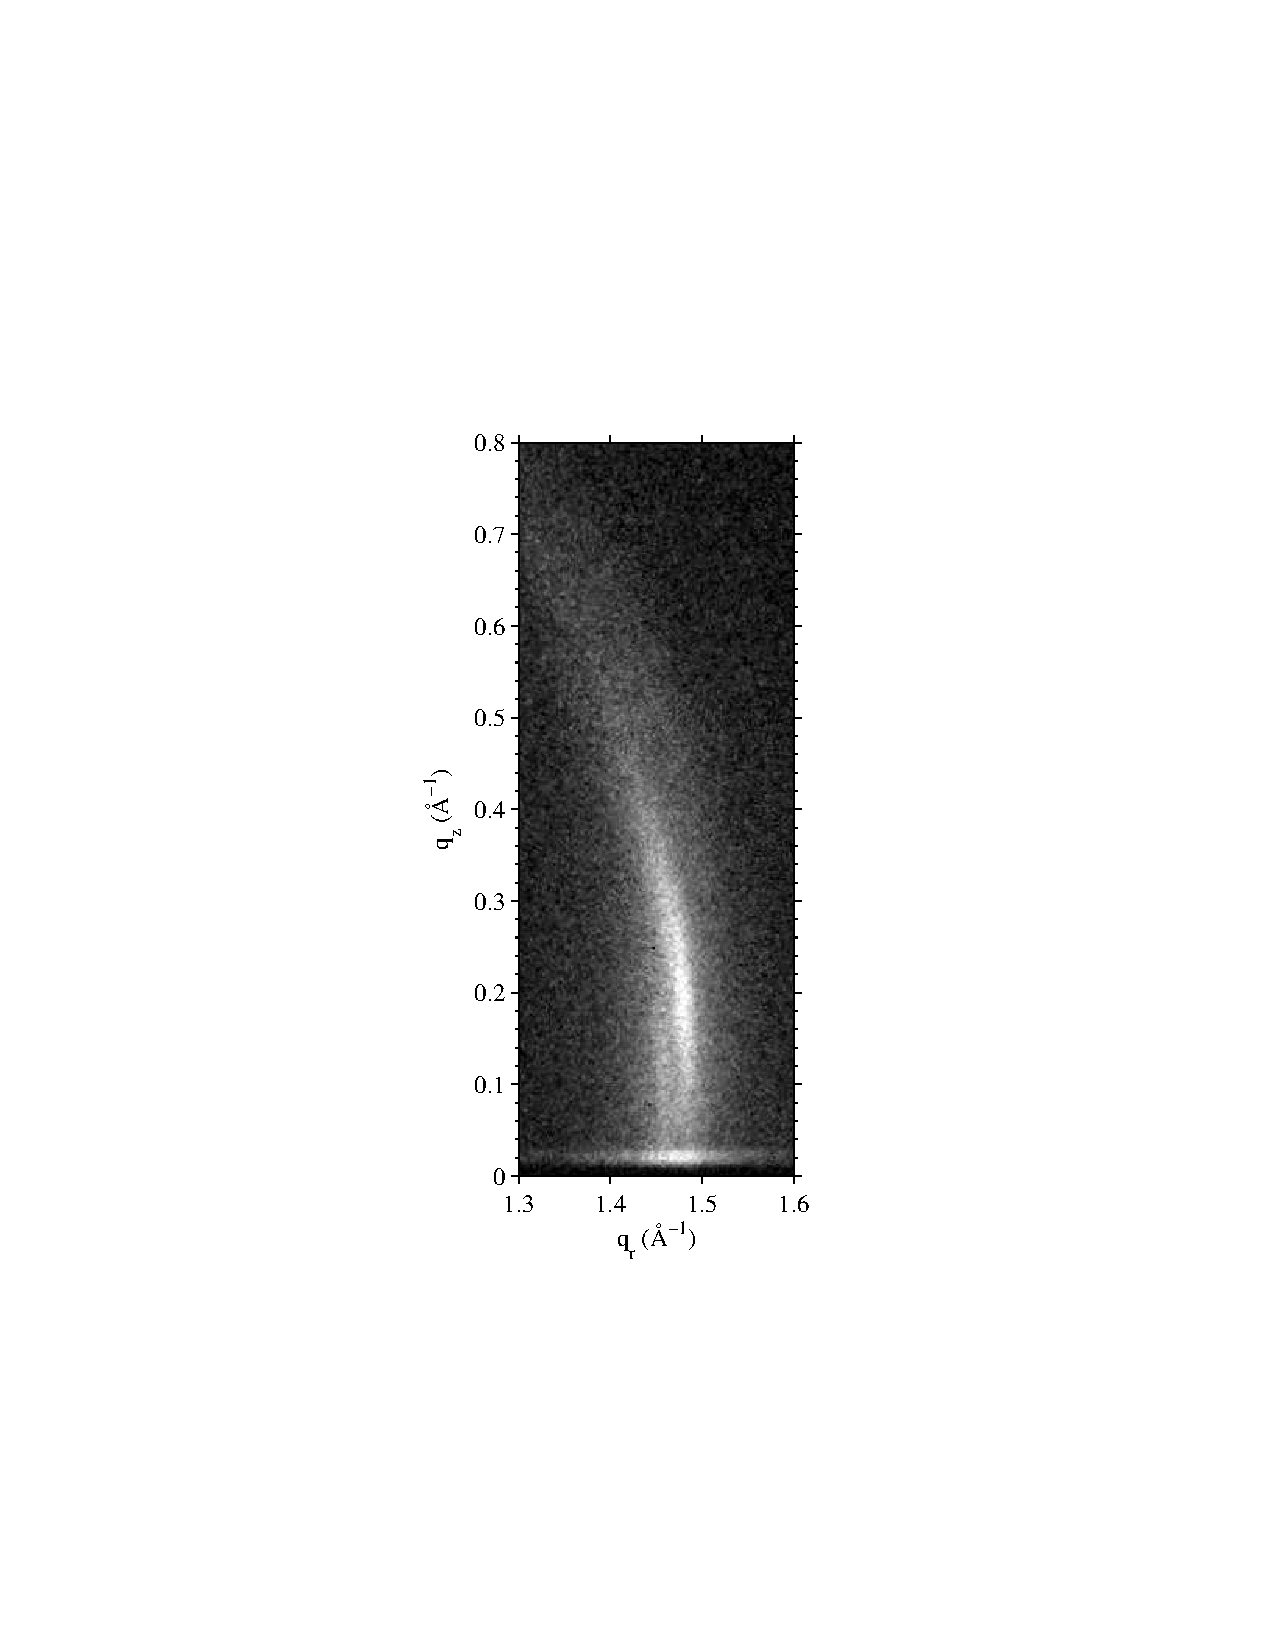
\includegraphics[trim=100 170 100 170,clip,width=\textwidth]{figures/ripple/NGIWAXS/dmpc1_enlarge}
  \caption{Enlarged view of the right image in Fig.~\ref{fig:NGIWAXS}. To show 
  smaller features around the peak, a different contrast is used.}
  \label{fig:NGIWAXS_enlarge}
\end{figure}

\begin{figure}[htbp]
  \centering
  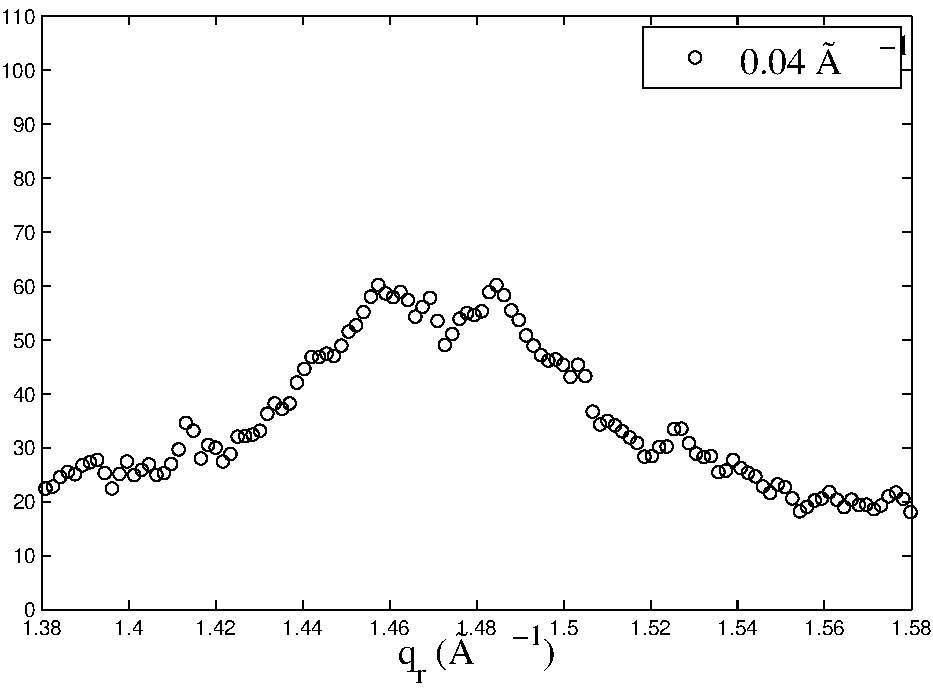
\includegraphics[width=0.3\textwidth]{figures/ripple/NGIWAXS/qrplot0}
  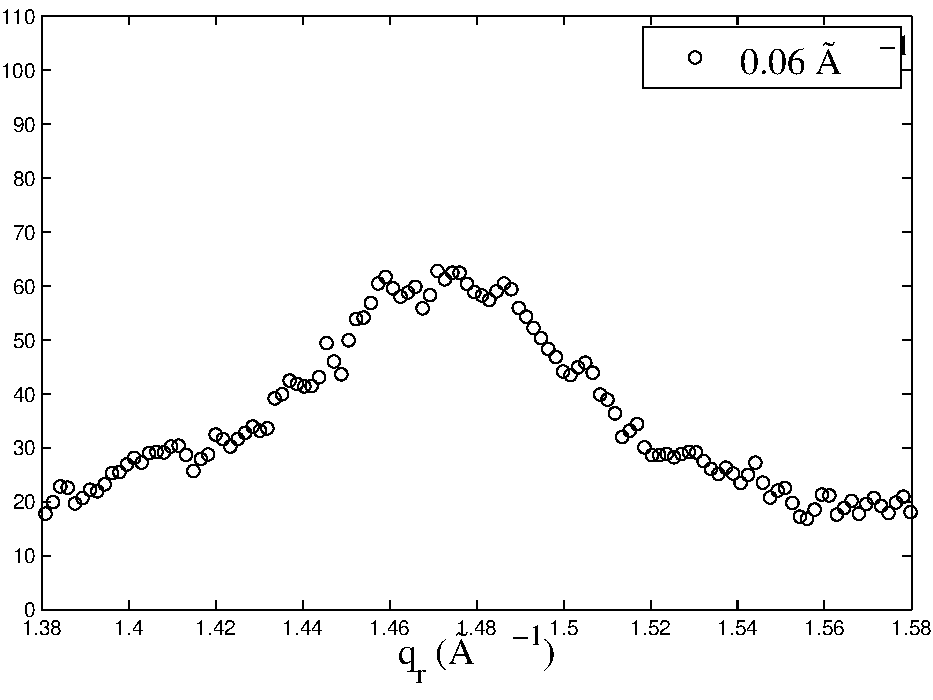
\includegraphics[width=0.3\textwidth]{figures/ripple/NGIWAXS/qrplot1}
  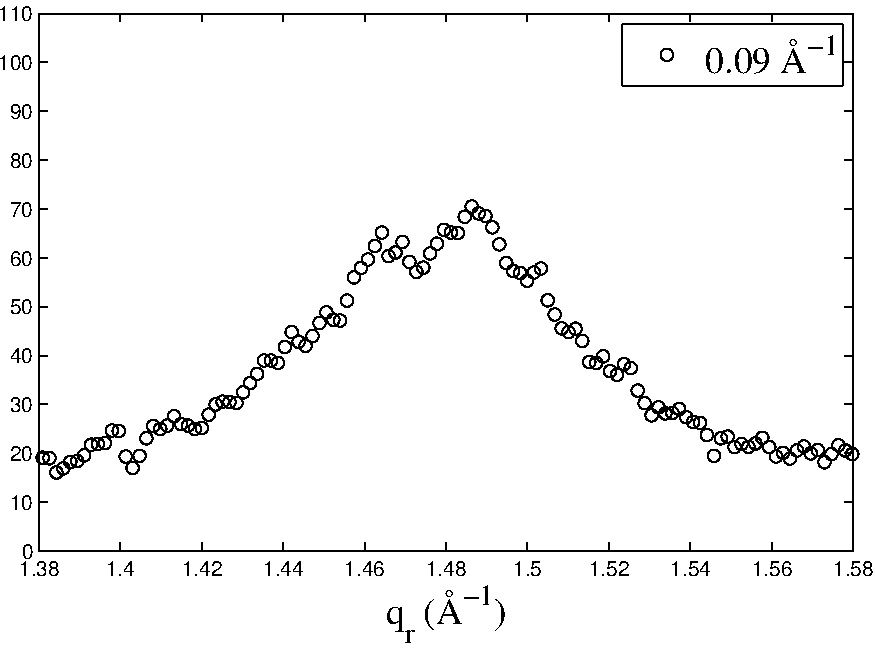
\includegraphics[width=0.3\textwidth]{figures/ripple/NGIWAXS/qrplot2}
  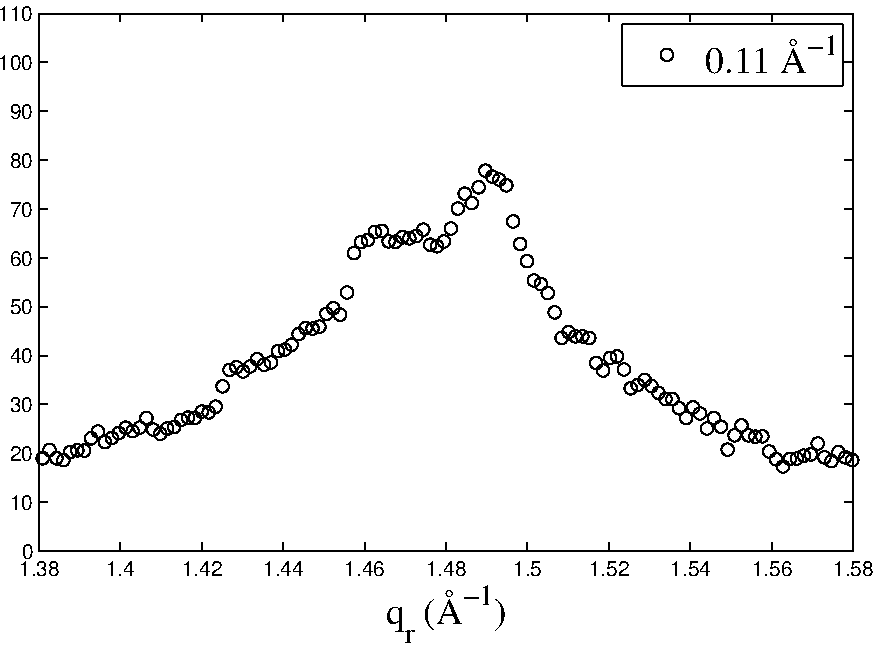
\includegraphics[width=0.3\textwidth]{figures/ripple/NGIWAXS/qrplot3}
  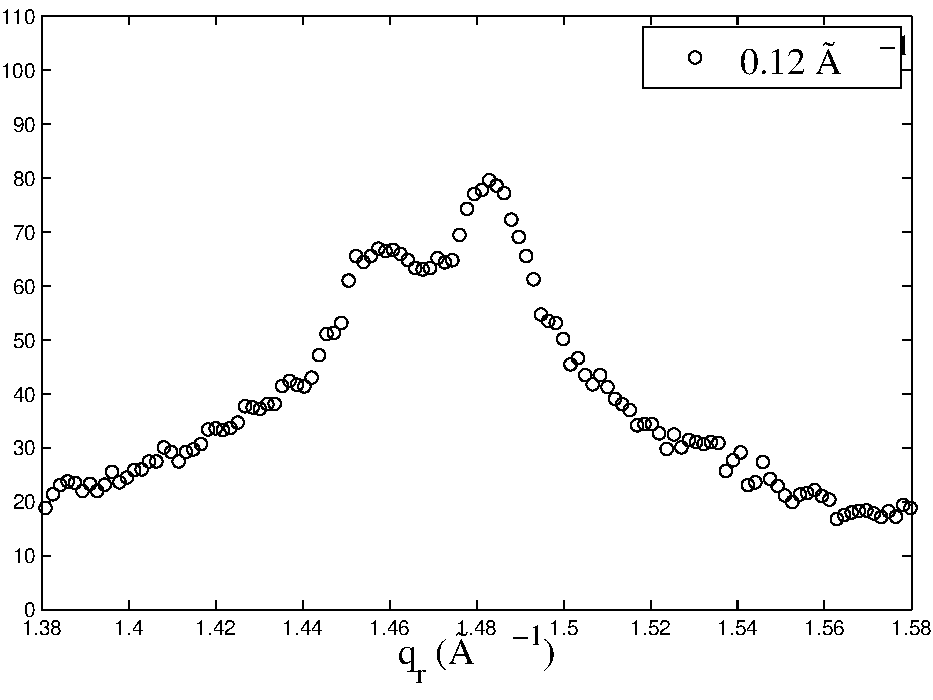
\includegraphics[width=0.3\textwidth]{figures/ripple/NGIWAXS/qrplot4}
  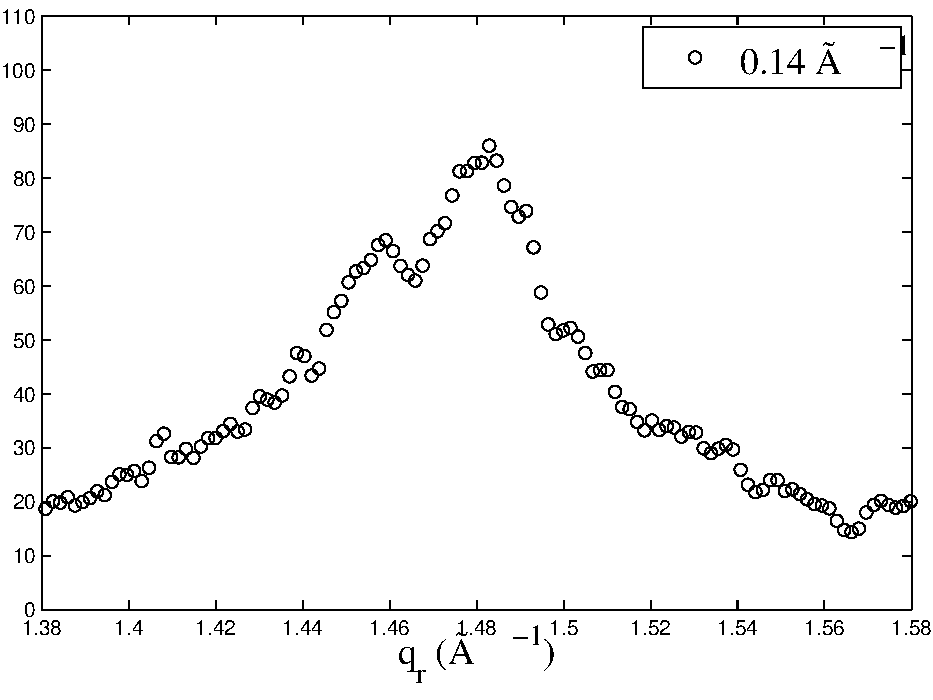
\includegraphics[width=0.3\textwidth]{figures/ripple/NGIWAXS/qrplot5}
  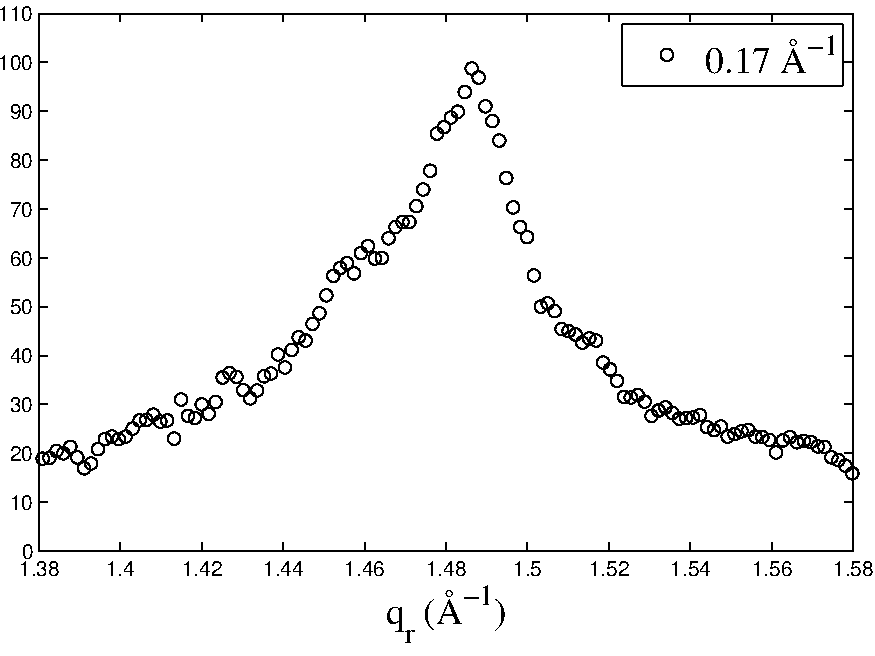
\includegraphics[width=0.3\textwidth]{figures/ripple/NGIWAXS/qrplot6}
  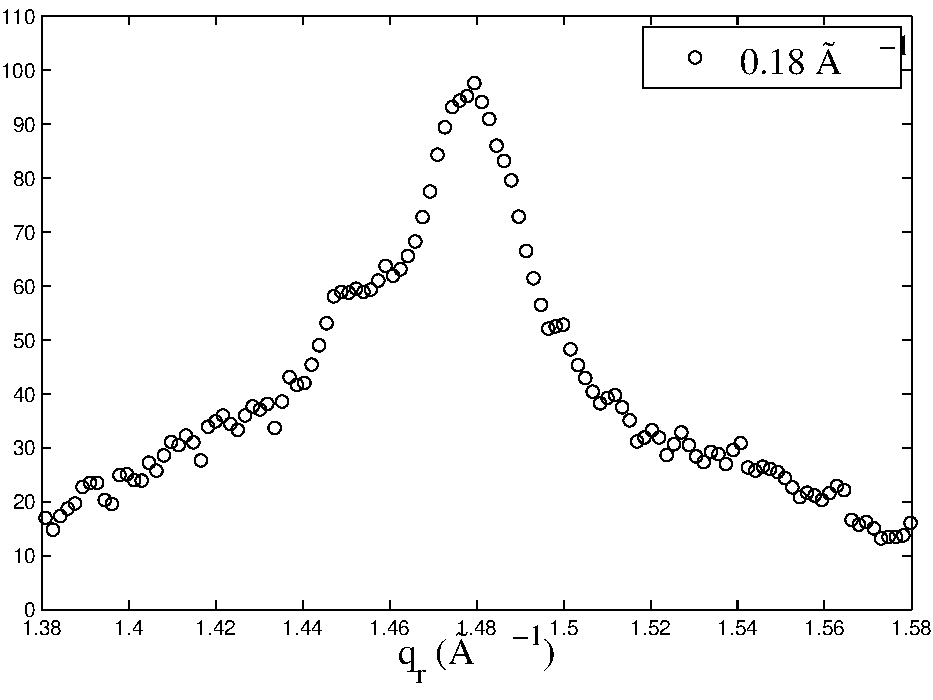
\includegraphics[width=0.3\textwidth]{figures/ripple/NGIWAXS/qrplot7}
  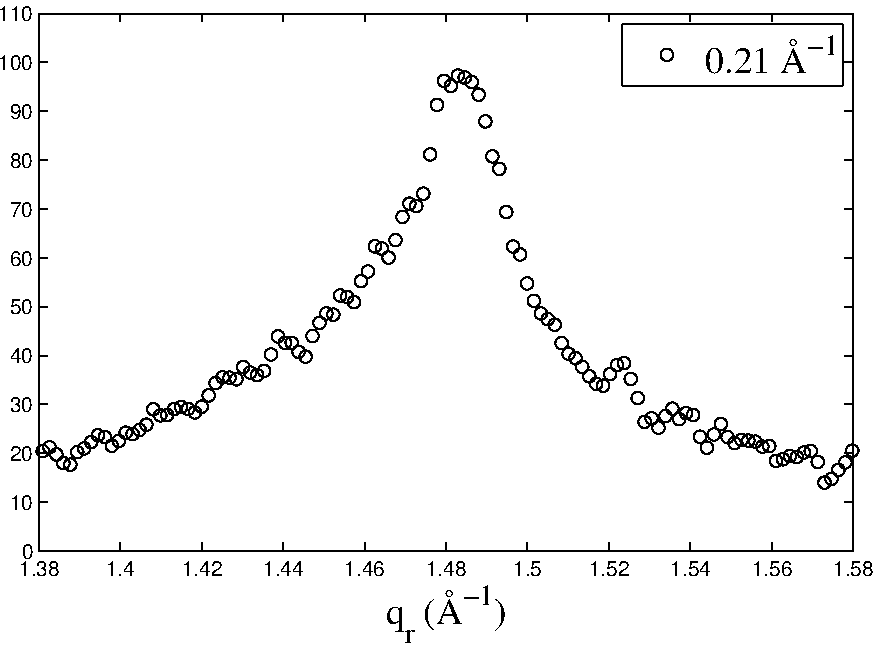
\includegraphics[width=0.3\textwidth]{figures/ripple/NGIWAXS/qrplot8}
  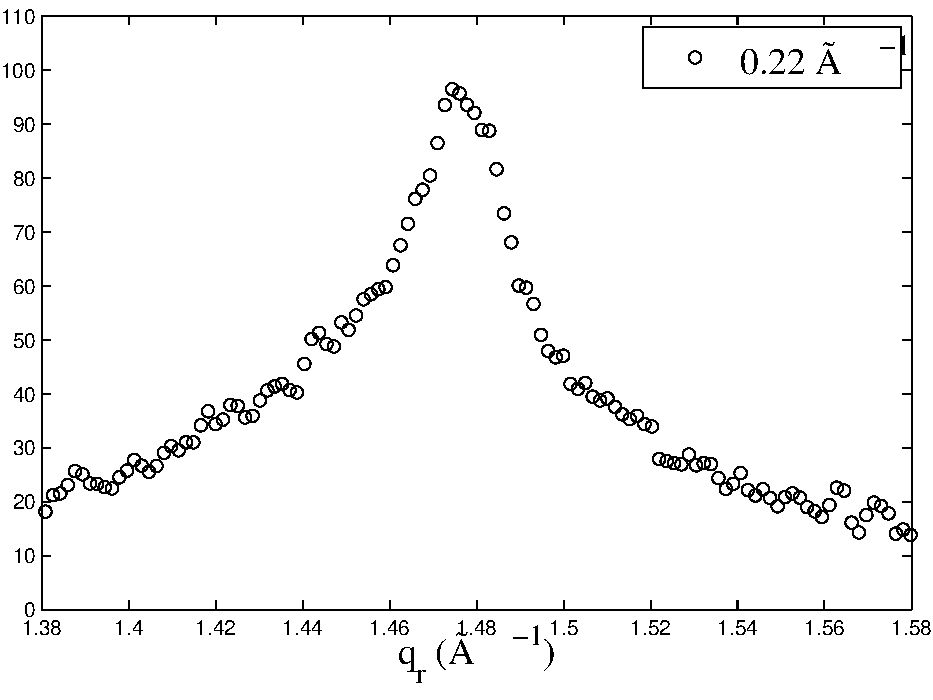
\includegraphics[width=0.3\textwidth]{figures/ripple/NGIWAXS/qrplot9}
  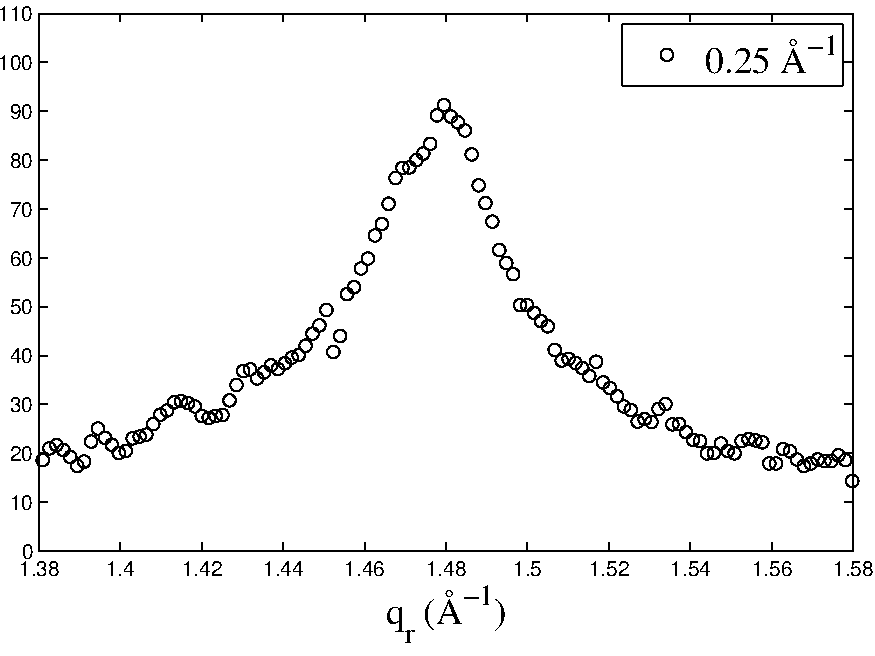
\includegraphics[width=0.3\textwidth]{figures/ripple/NGIWAXS/qrplot10}
  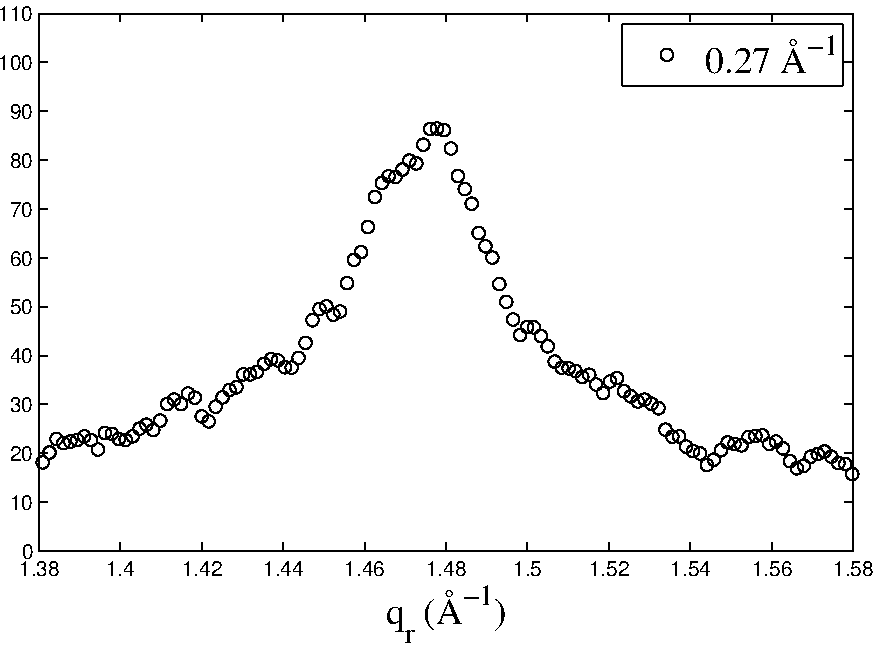
\includegraphics[width=0.3\textwidth]{figures/ripple/NGIWAXS/qrplot11}
  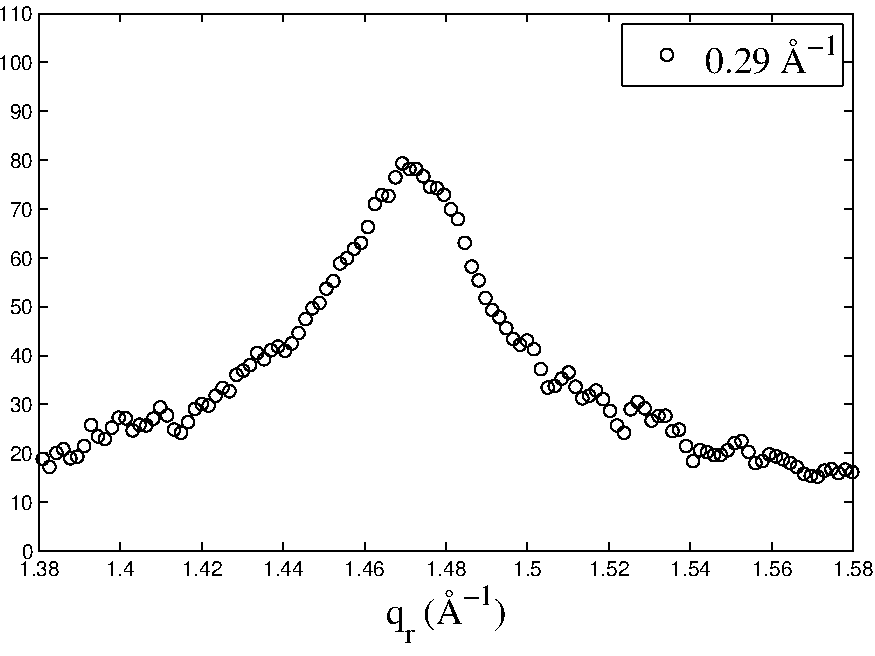
\includegraphics[width=0.3\textwidth]{figures/ripple/NGIWAXS/qrplot12}
  \includegraphics[width=0.3\textwidth]{figures/ripple/NGIWAXS/qrplot13}
  \caption{$q_r$ swaths, each averaged over 0.02 \AA$^{-1}$. 
  The center $q_z$ value of a swatch is shown in the figure legends.}
  \label{fig:qrplots}
\end{figure}

(some thought) Can we say that
the observed arc like scattering is not the mosaic spread, but
true sample scattering? Comment on the widths of the peaks observed.
Possibly make use of both low and high resolution data.
Apply the absorption correction. Show q swaths for various $\phi$.

\section{TWAXS: results}\label{sec:TWAXS_results}
Convert the image to $q$-space.
No strong order on the equator. 
Compare to NGIWAXS and comment on the absorption effect
in NGIWAXS data.

\section{Discussion}
Comparison with previous unoriented/oriented stuff.

\section{Conclusion}
Future possible experiments
include the high resolution transmission experiment, where both geometric 
broadening and energy dispersion are minimized. The expected resolution 
is the width of the X-ray beam, which is about 3 pixels. This experiment 
doubles the best resolution achieved in this work. 
Another slightly different high resolution experiment is to use silicon 
crystal analyzer downstread of the sample, which completely remove geoemtric
boradening. The downside of this type of high resolution experiment is that
only one point in q-space is probed at any given exposure, so to get a full
2D map of wide angle scattering is time consuming.  
